\documentclass[12pt,twoside,openright]{report}
\usepackage{amsmath, amssymb, amscd, amsthm, amsfonts}
\usepackage[a4paper]{geometry}
\usepackage[utf8]{inputenc}
%	\usepackage[T1]{fontenc}
\usepackage{graphicx}
\graphicspath{ {./images/} }
\usepackage{hyperref}
\usepackage[italian]{babel}
\usepackage{tikz}
\usetikzlibrary{shapes, arrows.meta, positioning}
\usepackage{listings}
\usepackage{xcolor}
\usepackage{circuitikz}
\usepackage{frontespizio}
\usepackage{minted}
\definecolor{LightGray}{gray}{0.9}
\usemintedstyle{tango}
\usepackage{subcaption}


\usepackage[backend=biber,sorting=none]{biblatex}
\usepackage[autostyle,italian=guillemets]{csquotes}
\usepackage{guit}
\usepackage{latexsym}
\addbibresource{./bibliografia.bib}


\definecolor{codegreen}{rgb}{0,0.6,0}
\definecolor{codegray}{rgb}{0.5,0.5,0.5}
\definecolor{codepurple}{rgb}{0.58,0,0.82}
\definecolor{backcolour}{rgb}{0.95,0.95,0.95}
\definecolor{orange}{rgb}{0.88, 0.55, 0.24}

\lstdefinestyle{mystyle}{
    backgroundcolor=\color{backcolour},   
    commentstyle=\color{green},
    keywordstyle=\color{orange},
    numberstyle=\tiny\color{black},
    stringstyle=\color{red},
    basicstyle=\ttfamily\footnotesize,
    breakatwhitespace=false,         
    breaklines=true,                 
    captionpos=b,                    
    keepspaces=true,                 
    numbers=left,                    
    numbersep=5pt,                  
    showspaces=false,                
    showstringspaces=false,
    showtabs=false,                  
    tabsize=2
}

\lstset{style=mystyle}

%\oddsidemargin 0pt
%\evensidemargin 0pt
%\marginparwidth 40pt
%\marginparsep 10pt
%\topmargin -20pt
%\headsep 10pt
%\textheight 8.7in
%\textwidth 6.65in
%\linespread{1.2}

\title{Stabilizzazione nel piano di Gough-Stewart}
\author{Daniele Facco}
\date{}

%\newtheorem{theorem}{Theorem}
%\newtheorem{lemma}[theorem]{Lemma}
%\newtheorem{conjecture}[theorem]{Conjecture}

%\newcommand{\rr}{\mathbb{R}}

%\newcommand{\al}{\alpha}
%\DeclareMathOperator{\conv}{conv}
%\DeclareMathOperator{\aff}{aff}

\begin{document}


  \begin{frontespizio}
    \Logo[3cm]{logo.jpg}
    \Istituzione {Università degli Studi di Trieste}
    \Divisione{dipartimento di Ingegneria e Architettura}
    \Corso [Laurea]{Ingegneria Elettronica e Informatica}
    \Titolo {Stabilizzazione nel piano di Gough-Stewart}
    \Candidato {Daniele Facco}
    \Relatore {Prof. Stefano Marsi}
    \Annoaccademico {2020-2021}
  \end{frontespizio}

%\maketitle
\newpage
\hbox{}
\newpage
\tableofcontents
\addtocontents{toc}{~\hfill\textbf{Pagina}\par}
\newpage

%\begin{abstract}
%Studio della piattaforma di Stewart e dei suoi componenti.
%\end{abstract}


\chapter*{Introduzione}\label{intro}
\addcontentsline{toc}{section}{Introduzione}
La tesi tratta della realizzazione di una piattaforma di Gough-Stewart, una particolare tipologia di robot esapode parallelo dotato di sei gradi di libertà e del relativo controllore in retroazione negativa atto a stabilizzare una pallina sul piano stesso.
Tale ricerca è stata svolta per approfondire il funzionamento di questo particolare sistema meccanico, che risulta essere una generalizzazione di moltissimi sistemi di largo impiego, soprattutto in ambito industriale. L'applicazione a un problema di stabilizzazione è quindi un ottimo modo per dimostrare le capacità e la flessibilità di questa tecnologia. %Per ottenere questo risultato sono state impiegate diverse tecnologie, come un microprocessore Arduino, dei servomotori e un piano resistivo. %La realizzazione del progetto si concentra su diversi aspetti:
Una volta completata la realizzazione sarà quindi possibile procedere a testare il sistema con diverse analisi, sia del comportamento statico, con la valutazione della risposta al gradino, sia del comportamento dinamico, studiando il moto della pallina all'assegnazione di diversi tracciati, realizzati a partire dalle figure di Lissajous. L'obbiettivo del lavoro è quindi avere un sistema di controllo robusto, in grado di resistere ai disturbi esterni, e perfettamente capace di eseguire un controllo dinamico della pallina a una discreta velocità entro un margine di errore quanto più ridotto possibile.

Vista la diversità degli argomenti di ricerca trattati, questi sono stati divisi in diverse sezioni, dove i capitoli \ref{tecnologie}, \ref{pianostewart} e \ref{controllopalla} trattano il problema soffermandosi principalmente sul punto di vista teorico mentre i capitoli \ref{realizzazionepratica} e \ref{risultati} hanno un approccio decisamente più pratico. 
\begin{itemize}
\item Il capitolo \ref{tecnologie} tratta nel dettaglio delle varie tecnologie impiegate nella realizzazione, come i servomotori, il microprocessore e il piano resistivo, soffermandosi in particolare sulla realizzazione del chip di controllo del piano resistivo. 
\item Il capitolo \ref{pianostewart} dà innanzitutto una breve descrizione storica dello sviluppo della piattaforma e delle caratteristiche dei robot seriali e paralleli, per poi passare alla descrizione matematica completa e alla realizzazione dell'algoritmo di controllo in cinematica inversa. 
\item Il capitolo \ref{controllopalla} descrive innanzitutto in modo generale il controllore PID, per poi passare ad una analisi più approfondita del problema in questione e dei miglioramenti impiegati. 
\item Il capitolo \ref{realizzazionepratica} tratta diversi punti tra cui l'assemblaggio della piattaforma stessa, la programmazione in linguaggio \texttt{C} dei vari algoritmi di filtraggio e di controllo, la realizzazione del setpoint che esegua le figure di Lissajous e la taratura. 
\item Il capitolo \ref{risultati} infine mostra i risultati e le capacità del sistema con diverse figure che permettono di valutare le prestazioni del sistema.
\end{itemize}

%\begin{itemize}\item La formalizzazione matematica del modello e l'analisi del sitema.\item L'assemblaggio e la realizzazione dell'elettronica di controllo.\item L'interfacciamento e il filtraggio del segnale proveniente dal piano resistivo.\item L'implementazione software del controllore PID.\item La taratura del controllore realizzato.\end{itemize}



\chapter{Tecnologie impiegate}\label{tecnologie}

\section{Piattaforma Arduino}\label{arduino}
L'intero progetto si basa su una unità di controllo centrale, è quindi fondamentale impiegare un processore con discrete capacità elaborative. Una scelta molto comune, è quella utilizzare schede Arduino che con il vantaggio di essere OpenHardware hanno raggiunto una discreta ubiquità nel settore, anche grazie ad un ambiente di sviluppo completo e ad un sistema di librerie molto supportato dai produttori di componenti. La scheda impiegata è Arduino UNO con un processore ATmega328P, il quale permette di avere una frequenza di clock di $16MHz$, perfettamente in grado di gestire la rapidità di calcolo richiesta dal progetto. Alla scheda impiegata è stato poi montato uno "shield", un componente che rimappa i pin in modo più conveniente per connettere dispositivi quali: servomotori, display LCD, moduli bluetooth e altri, oltre che facilitare l'alimentazione esterna tramite appositi morsetti. I pin impiegati sono divisi in base alla periferica:
\begin{itemize}
\item Il controllo dei servomotori, svolto dai pin con capacità PWM ovvero 3, 5, 6, 9, 10 e 11.
\item Il controllo del piano resistivo da 12, 13 e A0.
\item La lettura del joystick, tramite l'impiego di A5, A6 e 7.
\end{itemize}

\section{Servomotori}\label{servomotori}
I servomotori sono l'elemento principale nella realizzazione della piattaforma di Stewart. Sono presenti sei attuatori, controllati in modalità PWM dalla scheda Arduino tramite la libreria \texttt{Servo.h}. L'interpretazione del segnale in ingresso è gestita da un apposito chip di controllo che lo trasforma e lo invia a un motore DC brushless, che tramite un gearbox ad alta riduzione fa ruotare l'asse. La rotazione dell'asse è inoltre recepita dal controllore interno tramite un potenziometro, dando quindi la possibilità di aumentare la coppia se il setpoint non è raggiunto. L'intero sistema è riassunto in figura \ref{fig:servo}. 
\begin{figure}[h!]
\centering
\scalebox{1}{
\begin{tikzpicture}[font=\small,thick]

\filldraw  [fill=blue!50](0cm,0cm) rectangle (4cm,3cm);
\filldraw [fill=white](0.25cm,0.25cm) rectangle (1.5cm,2.25cm)node[xshift=-0.625cm, yshift=-1cm]{DC};
\filldraw [fill=black] (2.5cm,2cm) rectangle (3cm,3.5cm);
\filldraw  [fill=white](0.25cm,2.25cm) rectangle (3.75cm,2.75cm)node[xshift=-1.75cm, yshift=-0.25cm]{Gearbox};
\filldraw [fill=white] (2.25cm,2cm) rectangle (3.25cm,1.5cm)node[xshift=-0.5cm, yshift=0.25cm]{Pot.};
\filldraw [fill=white] (2cm,0.25cm) rectangle (3.5cm,1.25cm)node[xshift=-0.75cm, yshift=-0.5cm]{Chip};
\draw [line width=2pt](2,0.5) -- (1.5,0.5);
\draw [line width=2pt](2,1) -- (1.5,1);
\draw [line width=2pt](2.5,1.25) -- (2.5,1.5);
\draw [line width=2pt](2.75,1.25) -- (2.75,1.5);
\draw [line width=2pt](3,1.25) -- (3,1.5);
\draw [line width=2pt](3.5,0.5) -- (7,0.5)node[anchor= south]{GND};
\draw [line width=2pt](3.5,0.75) -- (6,0.75)node[anchor= south]{5V};
\draw [line width=2pt](3.5,1) -- (5,1)node[anchor= south]{Segnale};

\end{tikzpicture}
}
\caption{Componenti del servomotore.} \label{fig:servo}
\end{figure}
A causa del loro elevato rapporto di riduzione questi componenti possono produrre una coppia elevata\footnote{I servomotori impiegati possono sollevare una massa di $3,5kg$ con una manovella di lunghezza nominale $1cm$.}, questo aspetto  non va sottovalutato ed è sempre necessario gestire l'evenienza di uno sforzo durante l'operazione della piattaforma.
Il segnale inviato ai servomotori è periodico, di periodo $20ms$ e presenta uno stato on/off a livello logico per un tempo prefissato a seconda della posizione richiesta. In figura \ref{fig:servocontrol} è descritto il segnale PWM al variare dell'angolo richiesto. 
Il controllo di questi elementi è svolto dal processore tramite uno shield che ne facilita l'installazione. Una nota particolare va fatta in merito alla potenza richiesta dai servomotori, nonostante il loro consumo in stato "idle" sia di circa $10mW$, durante il movimento o lo sforzo questo può superare i $500mW$. É quindi necessaria una alimentazione esterna che sia in grado di fornire almeno $1A$ a $5V$, in quanto la scheda alimentata tramite usb dalla presa del computer può ricevere al massimo $500mA$. Una nota particolare va fatta in merito alla scelta di impiegare servomotori rispetto agli stepper, mentre i primi presentano un posizionamento assoluto, determinato dal segnale PWM e un feedback continuo sulla posizione, i secondi si basano su un posizionamento relativo, sarebbe quindi necessaria un'azione di calibrazione ad ogni accensione del dispositivo, che è preferibile evitare.
\begin{figure}[h!]
\centering
\scalebox{1.1}{
\begin{tikzpicture}[font=\small,thick]

\draw [dashed, gray] (2.375cm,-4.05cm) -- (2.375cm,1.5cm)node[anchor= south]{$20ms$};
\draw [dashed, gray] (4.75cm,-4.05cm) -- (4.75cm,1.5cm)node[anchor= south]{$40ms$};
\draw [dashed, gray] (7.125cm,-4.05cm) -- (7.125cm,1.5cm)node[anchor= south]{$60ms$};
 
\filldraw [fill=green!50] (0,0) rectangle (0.11875,1)node[anchor=west, gray]{$1ms$};
\filldraw [fill=green!50] (2.375,0) rectangle (2.375+0.11875,1);
\filldraw [fill=green!50] (4.75,0) rectangle (4.75+0.11875,1);
\filldraw [fill=green!50] (7.125,0) rectangle (7.125+0.11875,1)node[anchor=west, gray , xshift= 1.5cm, yshift= -0.5cm]{$...$};

\filldraw [fill=yellow!50] (0,-2) rectangle (0.1781,1-2)node[anchor=west, gray]{$1.5ms$};
\filldraw [fill=yellow!50] (2.375,-2) rectangle (2.375+0.1781,1-2);
\filldraw [fill=yellow!50] (4.75,0-2) rectangle (4.75+0.1781,1-2);
\filldraw [fill=yellow!50] (7.125,0-2) rectangle (7.125+0.1781,1-2)node[anchor=west, gray , xshift= 1.5cm, yshift= -0.5cm]{$...$};

\filldraw [fill=red!50] (0,-4) rectangle (0.2375,1-4)node[anchor=west, gray]{$2ms$};
\filldraw [fill=red!50] (2.375,0-4) rectangle (2.375+0.2375,1-4);
\filldraw [fill=red!50] (4.75,0-4) rectangle (4.75+0.2375,1-4);
\filldraw [fill=red!50] (7.125,0-4) rectangle (7.125+0.2375,1-4)node[anchor=west, gray , xshift= 1.5cm, yshift= -0.5cm]{$...$};

\draw [-latex] (0cm,0cm) -- (0cm,1.5cm);
\draw [-latex] (0cm,0cm) -- (9.5cm,0cm)node[anchor= west]{$t$};

\draw [-latex] (0cm,-2cm) -- (0cm,-0.5cm);
\draw [-latex] (0cm,-2cm) -- (9.5cm,-2cm)node[anchor= west]{$t$};

\draw [-latex] (0cm,-4cm) -- (0cm,-2.5cm);
\draw [-latex] (0cm,-4cm) -- (9.5cm,-4cm)node[anchor= west]{$t$};

\filldraw [fill=black] (12,0.75) circle (3pt) node[xshift= -1cm] {$0^\circ$};
\filldraw [fill=black] (12,-1.25) circle (3pt) node[xshift= -1cm] {$90^\circ$};
\filldraw [fill=black] (12,-3.25) circle (3pt) node[xshift= -1cm] {$180^\circ$};

\draw [line width=1mm](12,0.75) -- (12cm,1.75cm);
\draw  [line width=1mm](12,-1.25) -- (13cm,-1.25cm);
\draw [line width=1mm](12,-3.25) -- (12cm,-4.25cm);

\draw (12,0.75) circle (7pt);
\draw (12,-1.25) circle (7pt);
\draw (12,-3.25) circle (7pt);

\end{tikzpicture}
}
\caption{Angolo del servomotore al variare del segnale PWM.} \label{fig:servocontrol}
\end{figure}

\section{Piano resistivo}\label{pianoresistivo}
Per attuare correttamente la stabilizzazione del piano è fondamentale l'impiego di un sistema resistente ai disturbi che sia in grado determinare, con la massima precisione possibile, la posizione della sfera da bilanciare. Questo può essere svolto impiegando diverse tecniche come matrici di laser, rilevazione video o per l'appunto tramite l'uso di un piano resistivo.
É stato scelto di impiegare un digitalizzatore resistivo per il tracking della pallina in quanto è meno soggetto a disturbi ambientali, in particolare da effetti ottici, rispetto alla matrice laser e alla rilevazione video.
Il tracking video avrebbe inoltre richiesto un notevole incremento della complessità del sistema, necessitando di un SOC completo e di software dedicato come OpenCV.
\begin{figure}[h!]
\centering
\scalebox{0.75}{
\begin{tikzpicture}[font=\small,thick]
 

\filldraw [fill=cyan!50](0cm,0cm) rectangle (0.5cm,5cm);
\draw (0.5cm,0cm) rectangle (0.7cm,5cm);
\filldraw[ draw = red!50, very thick, -{Triangle[width=2cm, length= 1cm]}, line width = 1cm] (-4.0,2.5)node[xshift= 1.8cm]{\resizebox{!}{0.35cm}{$Pressione$}} -- (0.0,2.5);
%\node[single arrow, draw=blue, fill=green, minimum width = 10pt, single arrow head extend=3pt, minimum height=10mm] {}(-4.0cm,2.5cm) to (0.0cm,2.5cm); % length of arrow
\draw (1.25cm,0cm) rectangle (1.5cm,5cm);
\filldraw [fill=cyan!50] (1.5cm,0cm) rectangle (2cm,5cm);
\filldraw [fill=black!50](1.25,4.5) arc (90:270:0.5cm);
\filldraw [fill=black!50](1.25,1.5cm) arc (90:270:0.5cm);
\end{tikzpicture}
}
\caption{Sezione del digitalizzatore resistivo.} \label{fig:sezione}
\end{figure}
\subsection{Tipologie e funzionamento di un piano resistivo}\label{tipofunz}
I piani resistivi sono generalmente identificati dal numero di connessioni in uscita, questo può generalmente essere quattro, cinque o otto. La versione a otto fili è una semplice evoluzione della variante a quattro e non sarà trattata in dettaglio. Questi dispositivi sono costituiti da due strati, di vetro o plastica, ricoperti da un sottile strato di ossido di indio-stagno\footnote{Materiale scelto appositamente per le ottime proprietà di trasparenza e conduzione.} e separati da minuscoli spaziatori, come rappresentato in figura \ref{fig:sezione}. 
La resistenza del conduttore è uniforme su tutta la superficie e alla pressione si forma un contatto tra i due strati che permette un passaggio di corrente. A seconda del punto di pressione si formerà un rapporto di partizione diverso, indicativo della posizione.
Nella versione a quattro fili su entrambi i piani si forma un gradiente di potenziale nelle direzioni rispettivamente \emph{x}, \emph{y} e ognuno dei due misura il potenziale dell'altro. Nella versione a cinque invece si ha un piano su cui viene alternata la direzione del gradiente mentre l'altro effettua la misura\cite{pianoresistivo}. La schematica del piano resistivo è rappresentata in figura \ref{fig:pianoresistivo}, dove le resistenze rosse indicano il potenziale letto dal contatto tra i due strati resistivi, caratteristico di una specifica posizione. Il valore di tensione letto sarà quindi inviato all'ADC della scheda Arduino, che effettuerà una quantizzazione a $10bit$, restituendo un valore da $0$ a $1023$, poi convertito in una posizione effettiva.
Nella realizzazione del progetto è stata impiegata la variante di piano resistivo a cinque fili.
\begin{figure}[h!]
\centering
\scalebox{0.28}{

\begin{circuitikz}[ultra thick]
\node[anchor=south west,inner sep=0] at (0,0) {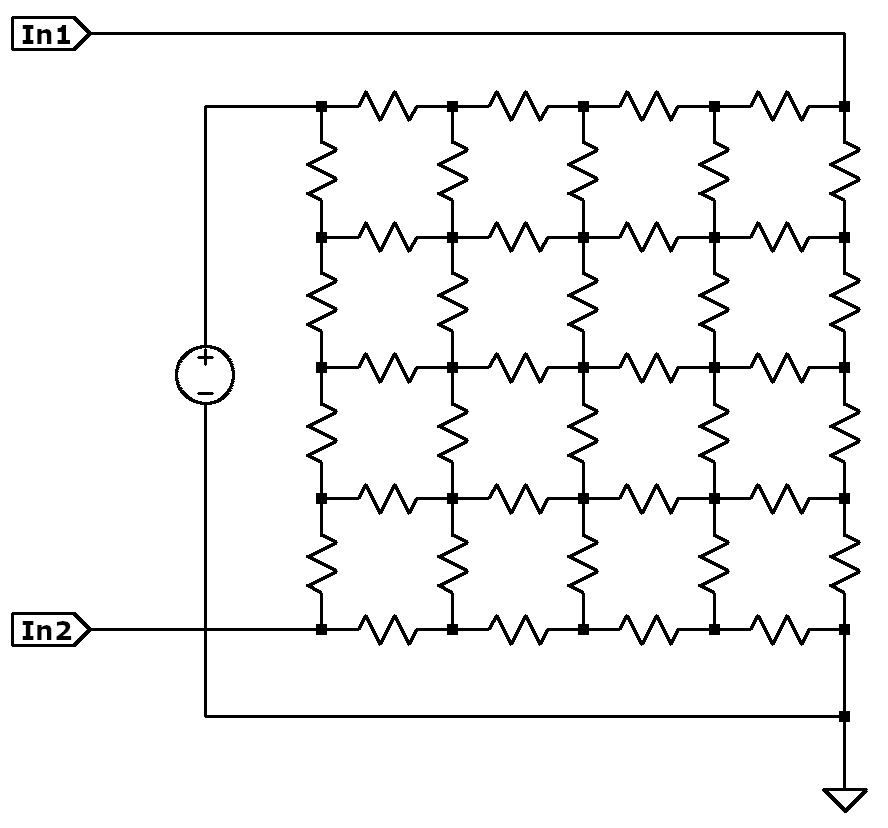
\includegraphics{5wireredo.png}};
 %\draw[red,ultra thick,rounded corners] (7.5,5.3) rectangle (9.4,6.2);

\scalebox{2}{
\filldraw [fill=red] (11.5,7) circle (5pt);
\draw [red, line width=2pt]
	(11.5,7) to[R,color=red] (13,8.5)
	(13,8.5) to[R,color=red] (14.5,10)
	(14.5,10) -- (16.5,10)node[anchor=west]{\large\textbf{Analog Out}};
;
}
\end{circuitikz}
}
\caption{Schema circuitale piano resistivo a cinque fili.} \label{fig:pianoresistivo}
\end{figure}

\section{Ponte ad H}\label{hbridge}
La necessità di impiegare un ponte ad H come circuito di driver è emersa in seguito ad una analisi preliminare delle specifiche del digitalizzatore resistivo. Si è infatti notato, in seguito a una misura di resistenza, che questa fosse di soli $100 \Omega$, quindi non compatibile con le periferiche dell'Arduino UNO, in quanto a $5V$ si andrebbe a richiamare una corrente di $50mA$ mentre la scheda è in grado di fornirne solo $20$. L'impiego del ponte ad H ed una sorgente di alimentazione esterna stabilizzata permette di pilotare opportunamente il piano tramite l'uso dispositivi attivi come BJT o MOSFET. Non disponendo del componente finito si è scelto di realizzarlo a partire dai singoli chip in seguito ad un'analisi accurata tramite software SPICE (figura \ref{fig:controllo}) e basandosi sul datasheet del ponte L298N\cite{l298n}. Nella scelta della tecnologia da impiegare sono stati preferiti i MOSFET per via della caduta di tensione Drain-Source quasi nulla nello stato di conduzione dovuta a una bassissima resistenza interna. 
\begin{figure}[h!]
\centering
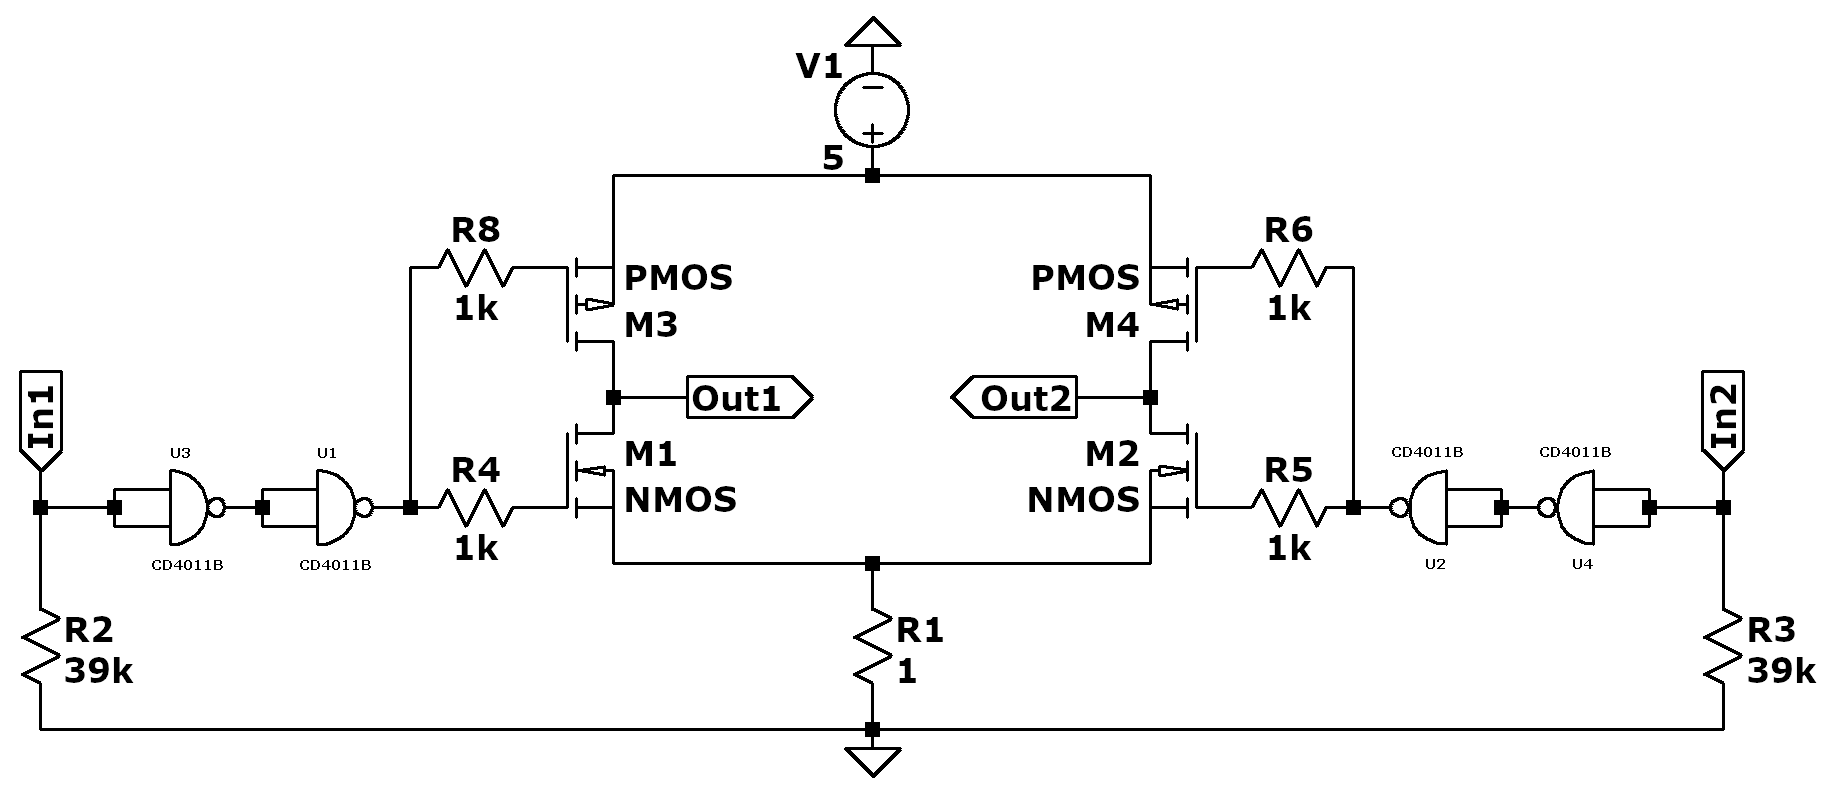
\includegraphics[width=\textwidth]{circuit3.png}
\caption{Schema elettrico del circuito di controllo.} \label{fig:controllo}
\end{figure}
I MOSFET scelti sono degli AO3400 e AO3401, rispettivamente nella configurazione N e P in quanto offrono ottime prestazioni relativamente alla $I_D$ e alla $R_{DS}$\cite{ao3400}\cite{ao3401}. Da un'analisi del sistema di controllo richiesto dal piano resistivo si è deciso di rinunciare alla capacità di gestire individualmente i singoli MOSFET favorendo due linee di controllo che possano commutare tra gli stati High/Low. Sono state inoltre impiegate delle porte logiche NAND con lo scopo di migliorare il pilotaggio dei MOSFET da parte di Arduino oltre che per disaccoppiare la logica di controllo dallo stadio di potenza, pratica comune anche nel caso del L298N. Come chip per le porte NAND si è scelto un TC4011BP, questo fornisce in un singolo package quattro porte logiche che sono state configurate come invertenti in cascata, principalmente per una questione di convenienza, nel caso in cui si fosse reso necessario impiegare il segnale negato\cite{TC4011BP}. Sono state poi inserite alcune resistenze, tra cui: 
\begin{itemize}
\item Una resistenza da $1\Omega$ verso ground per limitare la corrente di shoot-through\footnote{Conduzione simultanea di entrambi i MOSFET su un ramo durante la commutazione che porta alla creazione di un corto diretto tra alimentazione e massa.} durante la commutazione.
\item Due resistenze da $39k\Omega$ che dagli ingressi sono collegate verso ground, come pull down, per evitare che questi possano rimanere flottanti vista l'alta impedenza di ingresso delle porte NAND.
\item Quattro resistenze da $1k\Omega$ sui gate dei MOS, aggiunte in maniera preventiva nel caso si fosse verificato uno shoot-through importante per pilotare una linea di ritardo con lo scopo di interdire la formazione di un cammino diretto verso massa.
\end{itemize}
Da una successiva analisi all'oscilloscopio si è constatato che gli impulsi di corrente dovuti al cammino diretto sono estremamente brevi, rientrando ampiamente nelle specifiche dei MOSFET impiegati. Le quattro resistenze ai gate sono state quindi lasciate anche se non necessarie in quanto non peggiorano in modo sostanziale la costante dei tempi dovuta alla capacità di ingresso dei MOSFET che risulta essere come in equazione \ref{timeconstant}.
\begin{equation}\label{timeconstant}
\tau=R\cdot C = 1\times 10^3 \cdot 630\times 10^{-12}=630 ns
\end{equation}
Quindi del tutto ininfluente rispetto alle specifiche del progetto.

\section{Joystick analogico}\label{joystick}
Per facilitare e rendere più intuitivo il controllo del sistema è stato impiegato un joystick analogico. Questo dispositivo è costituito da due potenziometri montati ortogonalmente negli assi $x$ e $y$ oltre che da un piccolo switch momentaneo. I segnali analogici generati dai due potenziometri vengono digitalizzati dall'ADC del processore mentre l'interruttore viene letto dall'input digitale. Tramite questi dati sarà possibile avere un controllo diretto del piano ed assegnare dei setpoint in maniera arbitraria.

\newpage

\chapter{Piattaforma di Gough-Stewart}\label{pianostewart}



\section{Descrizione}\label{piattaformastewart}
La piattaforma di Gough-Stewart è un particolare sistema meccanico realizzato, per la prima volta nel 1954, dall'ingegnere britannico E. Gough (figura \ref{fig:gough}) e successivamente portata alla notorietà tramite la pubblicazione di un paper nel 1965 da parte di D. Stewart dal titolo "A Platform with Six Degrees of Freedom"\cite{stewart1965platform}. Il sistema è qui descritto come un robot esapode, ovvero costituito da una base, su cui sono posizionati sei attuatori di vario tipo, collegati alla piattaforma superiore mediante giunti snodabili. Il progetto originale prevedeva l'uso di attuatori prismatici, ovvero pistoni lineari che presentano un solo grado di libertà, offrendo numerose proprietà relative alla precisione a alla stabilità. Nella realizzazione del progetto si è però preferito seguire una strada alternativa ed impiegare servomotori, i quali presentano il vantaggio di essere certamente più economici rispetto agli attuatori prismatici ma il sistema risultante assume un grado di complessità decisamente superiore. Tramite opportune osservazioni matematiche sarà poi possibile risalire a un modello che rende equivalente l'impiego di attuatori rotativi a quello dei lineari, garantendo un controllo ottimale.
\begin{figure}[h!]
\centering
\scalebox{0.49}{
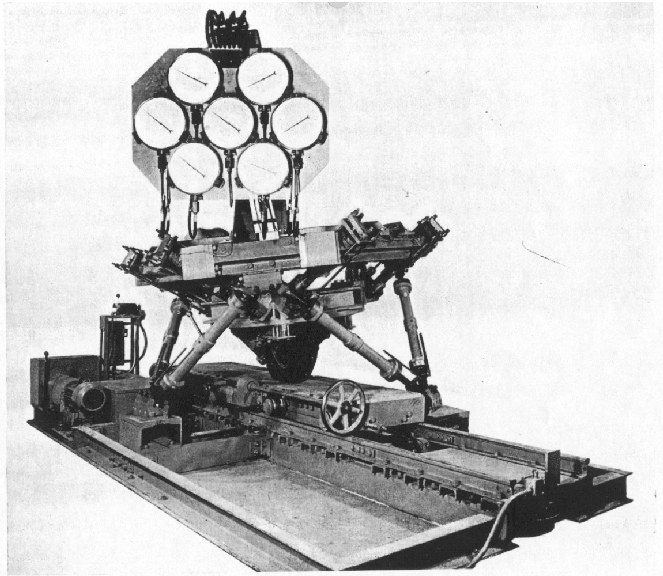
\includegraphics{gough.png}
}
\caption{La "universal rig" di Gough per testare pneumatici\cite{gough}.} \label{fig:gough}
\end{figure}

\section{Robot seriali e paralleli}\label{robotserialiparalleli}
È utile enunciare la differenza tra robot di tipo seriale e parallelo per comprendere le successive implicazioni a livello matematico. I robot seriali prevedono una serie di giunti snodabili controllati da attuatori, che spesso assumono le caratteristiche di un arto antropomorfo. 
Questi tipi di robot prendono spesso il nome di braccio meccanico e trovano ampia applicazione a livello industriale.
Nei robot paralleli invece, gli attuatori agiscono tutti sullo stesso elemento tramite giunti indipendenti. 
La piattaforma di Stewart ne è il principale esempio di cui si trovano applicazioni nella realizzazione di simulatori avanzati di volo, nei test relativi ai veicoli da parte delle case automobilistiche e a livello industriale nella sua configurazione ridotta a tre gradi di libertà, nota come delta-robot, nelle varie catene di montaggio\cite{bonev2001delta}.
%\footnote{Si nota come i delta-robot siano sostanzialmente delle versioni "limitate" della piattaforma di Stewart a soli 3 gradi di libertà.}
Entrambi i sistemi presentano sei gradi di libertà, indicati anche come $6DOF$, ma il problema matematico che li caratterizza è fondamentalmente opposto.
Lo schema logico dei problemi diretti e inversi è indicato in figura \ref{fig:direttoinverso}, dove $(\vartheta_1,\vartheta_2,...,\vartheta_n)$ indicano gli angoli dei servomotori e $(x,y,z,\varphi,\vartheta,\psi)$ la posizione dell'end-effector.
\begin{figure}[h!]
\centering
\scalebox{1.1}{
\begin{tikzpicture}[font=\small,thick]
 
\node[draw,
    minimum width=2cm,
    minimum height=1cm,
    text width=2cm, text centered
] (block1) {Sistema};

\draw [-latex] (-2cm,0cm)node[anchor=east]{$(\vartheta_1,\vartheta_2,...,\vartheta_n)$} -- (block1);
\draw [-latex] (block1) -- (2cm,0cm)node[anchor=west]{$(x,y,z,\varphi,\vartheta,\psi)$};
\draw node[yshift=-2cm,xshift=-3.5cm]{$(x,y,z,\varphi,\vartheta,\psi)=S(\vartheta_1,\vartheta_2,...,\vartheta_n)$};
\draw node[yshift=-1.25cm,xshift=0cm]{Problemi:};
\draw node[yshift=-2.5cm,xshift=-3.5cm]{Diretto};
\draw node[yshift=-2cm,xshift=3.5cm]{$(\vartheta_1,\vartheta_2,...,\vartheta_n)=S(x,y,z,\varphi,\vartheta,\psi)$};
\draw node[yshift=-2.5cm,xshift=3.5cm]{Inverso};

\end{tikzpicture}
}
\caption{Problemi diretti e inversi.} \label{fig:direttoinverso}
\end{figure}
Se nei robot seriali, noto l'orientamento degli attuatori, è facile risalire alla posizione dell'end effector; lo stesso non si può dire del problema inverso. Nota la posizione dell'end effector è infatti estremamente difficile risalire all'orientamento degli attuatori che permette raggiungere quella determinata locazione. Il problema della piattaforma di Stewart è esattamente l'opposto, è infatti complesso ottenere equazioni che ci permettano di descrivere le coordinate e la rotazione del piano al variare dell'angolo dell'attuatore rotativo mentre è più agevole risalire all'angolo dei servomotori a partire dalla posizione nota della piattaforma nello spazio impiegando semplici nozioni di trigonometria. Basti pensare che la soluzione diretta del problema prevede la risoluzione di un sistema di 30 equazioni nonlineari risolvibili in forma chiusa che possono arrivare ad avere fino a un massimo di 40 possibili soluzioni\cite{cinematicadiretta2}. Queste nozioni di cinematica sono riassunte nella tabella \ref{fig:tabella}.
\begin{table}[h!]
\centering
\begin{tabular}{c|cc}
   Problema     & Seriale   & Parallelo  \\ 
\hline
Diretto & Facile    & Difficile  \\
Inverso & Difficile & Facile    
\end{tabular}
\caption{Difficoltà problemi diretti e inversi} \label{fig:tabella}
\end{table}
Nello svolgimento successivo si è preferito risalire alle equazioni della cinematica inversa della piattaforma di Stewart in quanto permettono un controllo ottimale e allo stesso tempo un minor carico del microprocessore rispetto alla soluzione diretta. 



\section{Analisi piattaforma di Stewart con attuatori rotativi}\label{analisi}

Il problema della piattaforma di Stewart controllata da attuatori rotativi è fondamentalmente costituito da due sotto-problemi.
Il primo relativo alla determinazione delle lunghezze dei vettori che collegano la base alla piattaforma per ogni possibile posizione di quest'ultima, trattato nella sezione \ref{platform}. Il secondo si occupa invece dell'implementazione stessa dei servomotori, per via della complessità di descrizione del sistema biella manovella impiegato, trattato nella sezione \ref{rotation}. 

\begin{figure}[h!]
\centering

\scalebox{0.99}{
\begin{tikzpicture}

\filldraw[fill=yellow!50,rotate around={-10:(0,7cm)},xshift=2cm,yshift=1cm] (0,7cm) ellipse (4cm and 2cm);
\filldraw [fill=red!50](0,0) ellipse (5cm and 2.5cm);
\draw [-latex, thick] (0,0) -- node[anchor=south]{$\hat b_i$}(5cm,0);
\draw [-latex, thick] (0,0) -- node[anchor=east]{$\hat T$}(2.15cm,7.65cm);
\draw [-latex, thick] (0,0) -- node[anchor=north]{$\hat q_i$}(6.1cm,6.95cm);
\draw [-latex, thick] (5cm,0) -- node[anchor=west]{$\hat l_i$}(6.1cm,6.95cm);
\draw[-latex, thick,rotate around={-10:(0,7cm)},xshift=2cm,yshift=1cm] (0cm,7cm) -- node[anchor=south]{$\hat p_i$}(4cm,7cm);
\filldraw [fill=black] (0,0) circle (2pt) node[yshift= -0.25cm] {$O$} node[xshift= -2cm] {Base};
\filldraw [fill=black] (5cm,0) circle (2pt) node[anchor=west]{$B_i$};
\filldraw [fill=black] (2.15cm,7.65cm) circle (2pt) node[yshift= 0.25cm] {$O'$} node[xshift= -2cm] {Piattaforma};
\filldraw [fill=black] (6.1cm,6.95cm) circle (2pt) node[anchor=west]{$P_i$};
\draw [-latex, thick] (-1,-1.5) -- node[anchor=north]{$\hat i$}(0cm,-1.5cm);
\draw [-latex, thick] (-1,-1.5) -- node[anchor=east]{$\hat k$}(-1cm,-0.5cm);
\draw [-latex, thick,rotate around={-120:(-1,-1.5cm)}] (-1,-1.5) -- node[anchor=east]{$\hat j$}(-0.5cm,-1.5cm);

\draw [-latex, thick,rotate around={-10:(0,8.5cm)}] (0,8.5) -- node[anchor=north]{$\hat {i'}$}(1cm,8.5cm);
\draw [-latex, thick,rotate around={-10:(0,8.5cm)}] (0,8.5) -- node[anchor=east]{$\hat {k'}$}(0cm,9.5cm);
\draw [-latex, thick,rotate around={-130:(0,8.5cm)}] (0,8.5) -- node[anchor=east]{$\hat {j'}$}(0.5cm,8.5cm);

\end{tikzpicture}
}
\caption{Sistemi di rifermento e vettori nella piattaforma di Stewart.} \label{fig:sistema}
\end{figure}

\section{Analisi problema piattaforma}\label{platform}

Si definiscono due sistemi di riferimento cartesiani che caratterizzano il sistema, mostrati nella figura \ref{fig:sistema}, uno fisso per la base centrato in $O$ di versori $\hat{i},\hat{j},\hat{k}$ e uno variabile per la piattaforma centrato in $O'$ di versori $\hat{i'},\hat{j'},\hat{k'}$. Sono note le coordinate in tre dimensioni dei punti degli assi di rotazione dei servomotori $({B_i})$ e dei giunti della piattaforma $(P_i)$ quando questa è in posizione orizzontale a riposo rispetto al sistema di riferimento centrato nella base. Il problema consiste nel definire la posizione dei giunti della piattaforma nello spazio al variare di un set di valori $(x,y,z,\varphi,\vartheta,\psi)$ rispetto al riferimento fisso della base. I valori $(x,y,z,\varphi,\vartheta,\psi)$ precedentemente enunciati, si riferiscono alla posizione e rotazione nello spazio della piattaforma rispetto alla base; $(x,y,z)$ sono i valori del centro della piattaforma mentre $(\varphi,\vartheta,\psi)$ sono le rotazioni, rispettivamente roll, pitch e yaw (rollio, beccheggio e imbardata). Nell'analisi, si considerano separatamente gli effetti traslativi e rotativi.




\subsubsection{Analisi traslazione \boldmath$(x,y,z)$}\label{xyz}
Le variazioni in $(x,y,z)$ comportano una semplice traslazione dei punti della piattaforma, questa viene indicata con un vettore $\hat T$ che andrà poi a sommarsi alla variazione dovuta a $(\varphi,\vartheta,\psi)$.

\subsection{Analisi rotazione \boldmath$(\varphi,\vartheta,\psi)$}\label{ftp}
Per semplificare l'analisi si considerano, separatamente, gli effetti dovuti a queste tre componenti. Si studia il caso di solo rollio $(\varphi,0,0)$ per risalire alle coordinate di un punto $P:(x,y,z)$ rispetto alla base in seguito a una rotazione di $\varphi$ gradi che lo ha traslato nel punto $P':(x',y',z')$. Questo è rappresentato in figura \ref{fig:rot}, dove i sistemi cartesiani sovrapposti permettono di ricavare facilmente la relazione che lega le coordinate della piattaforma a quelle della base. 
Questo risultato è esprimibile matematicamente tramite l'applicazione lineare indicata in \eqref{sistema1}.
%Per fare ciò, è necessario ottenere un'applicazione lineare che permetta di passare dal sistema di coordinate della piattaforma al sistema di coordinate della base.
\begin{figure}
\centering
\scalebox{1.1}{
\begin{tikzpicture}
\draw [dashed,gray](1.5cm,0cm)node[anchor=north]{$y$} -- (1.5cm,2.6cm);
\draw [dashed,gray](0cm,2.6cm)node[anchor=east]{$z$} -- (1.5cm,2.6cm);
\draw [dashed,gray,rotate around={30:(0,0cm)}](2.6cm,0cm)node[anchor=north]{$y'$} -- (2.6cm,1.5cm);
\draw [dashed,gray,rotate around={30:(0,0cm)}](0cm,1.5cm)node[anchor=east]{$z'$} -- (2.6cm,1.5cm);

\draw [-latex](0,0) -- (4cm,0)node[anchor=north]{$\hat{j}$};
\draw [-latex](0,0) -- (0,4cm)node[anchor=east]{$\hat{k}$};

\draw [-latex,rotate around={30:(0,0cm)}](0,0) -- (4cm,0)node[anchor=north,xshift=0.25cm]{$\hat{j'}$};
\draw [-latex,rotate around={30:(0,0cm)}](0,0) -- (0,4cm)node[anchor=east]{$\hat{k'}$};

\draw[-latex,red,thick] (2.6,1.5) arc (30:59:3cm)node[anchor=west, xshift=0.3cm]{$Rotazione$};

\draw [rotate around={60:(0,0cm)}](0,0) -- (3cm,0)node[anchor=south]{$P'$};
\draw (0,0)node[xshift= 1.25cm,yshift= 0.25cm]{$\varphi$} -- (10mm,0mm) arc  (0:30:10mm)-- cycle;
\filldraw [-latex,fill=black] (0cm,0cm) circle (2pt) node[xshift=-0.25cm,yshift=-0.25cm]{$\hat{i}$};
\filldraw [-latex,fill=black] (1.5cm,2.6cm) circle (2pt);
\filldraw [-latex,fill=black] (2.6cm,1.5cm) circle (2pt)node[anchor=north,xshift=0.25cm]{$P$};

\draw (1.5cm,2.6cm)node[xshift= 0.2cm,yshift= -0.8cm]{$\varphi$} -- (1.5cm,2.1cm) arc  (270: 300:5mm)-- cycle;
\end{tikzpicture}
}
\caption{Punto $P$ ruotato di $\varphi$ gradi rispetto al sistema di riferimento della base.} \label{fig:rot}
\end{figure}
%Dallo studio della rotazione troviamo che:
\begin{equation}\label{sistema1}
\begin{cases} 
x=x' \\ 
y=y'cos(\varphi)-z'sin(\varphi) \\ 
z=y'sin(\varphi)-z'cos(\varphi)
\end{cases} 
\end{equation}
Per comodità di calcolo nei successivi passaggi il sistema \eqref{sistema1} viene riscritto in forma matriciale.
\begin{equation}\label{rx}
R_x(\varphi)=
\begin{bmatrix}
1 & 0 & 0\\
0 & cos(\varphi) & -sin(\varphi)\\
0 & sin(\varphi) & cos(\varphi)
\end{bmatrix}
\quad : \quad
\begin{bmatrix}
x \\
y \\
z 
\end{bmatrix}
=R_x(\varphi)\cdot\begin{bmatrix}
x' \\
y' \\
z' 
\end{bmatrix}
\end{equation}
Risultati analoghi si ottengono per le rotazioni indipendenti di $\vartheta$ e $\psi$:
\begin{equation}\label{ry}
R_y(\vartheta)=
\begin{bmatrix}
cos(\vartheta) & 0 & sin(\vartheta)\\
0 & 1 & 0\\
-sin(\vartheta) & 0 & cos(\vartheta)
\end{bmatrix}
\quad : \quad
\begin{bmatrix}
x \\
y \\
z 
\end{bmatrix}
=R_y(\vartheta)\cdot\begin{bmatrix}
x' \\
y' \\
z' 
\end{bmatrix}
\end{equation}
\begin{equation}\label{rz}
R_z(\psi)=
\begin{bmatrix}
cos(\psi) & -sin(\psi) & 0\\
sin(\psi) & cos(\psi) & 0\\
0 & 0 & 1\\
\end{bmatrix}
\quad : \quad
\begin{bmatrix}
x \\
y \\
z 
\end{bmatrix}
=R_z(\psi)\cdot\begin{bmatrix}
x' \\
y' \\
z' 
\end{bmatrix}
\end{equation}

Le singole matrici possono essere viste come applicazioni lineari, si procede quindi nella moltiplicazione di \eqref{rx}, \eqref{ry} e \eqref{rz} per ottenere una singola applicazione lineare composta detta matrice di rotazione globale $R_g$. Notare che nel prodotto tra matrici non vale la proprietà commutativa, bisogna quindi valutare attentamente l'ordine di moltiplicazione, altrimenti si otterrà una rotazione erronea. Nello svolgimento è stato scelto di svolgere le rotazioni attorno agli angoli di Eulero seguendo la convenzione ZYX\cite{matricerotazione} che prevede appunto la moltiplicazione ordinata delle matrici di rotazione di imbardata, beccheggio e rollio. I passaggi intermedi vengono omessi in quanto ripetono tre volte una semplice operazione di moltiplicazione tra matrici.
\begin{equation}\label{rg}
    R_g = R_z(\psi)\cdot R_y(\vartheta)\cdot R_x(\varphi)\\
\end{equation}
Il cui risultato è quindi:
\begin{equation}\label{rg}
\resizebox{0.9\hsize}{!}{$
\begin{bmatrix}
			cos(\vartheta)cos(\psi) & -cos(\varphi)sin(\psi)+sin(\varphi)sin(\vartheta)cos(\psi) & sin(\varphi)sin(\psi)+cos(\varphi)sin(\vartheta)cos(\psi)\\
			cos(\vartheta)sin(\psi) & cos(\varphi)cos(\psi)+sin(\varphi)sin(\vartheta)sin(\psi) & -sin(\varphi)cos(\psi)+cos(\varphi)sin(\vartheta)sin(\psi)\\
			-sin(\vartheta) & sin(\varphi)cos(\vartheta) & cos(\varphi)cos(\vartheta)
			\end{bmatrix}$}
\end{equation}
Moltiplicando il vettore $\hat{p_i}$, che congiunge il centro della piattaforma al giunto, per la matrice di rotazione \eqref{rg} si ottengono le coordinate del punto $P_i$ relative al sistema di riferimento della base. 

\subsection{Conclusione problema piattaforma}
Grazie ai risultati ottenuti nelle sezioni \ref{xyz} e \ref{ftp} si possono definire i vettori $\hat{q_i}$ che descrivono la posizione dei punti $P_i$ rispetto al centro del sistema di riferimento della base $O$ per ogni operazione rototraslativa.
\begin{equation}\label{qi}
\hat{q_i}=\hat{T}+R_g\cdot \hat{p_i}
\end{equation}
Una volta ottenuto questo vettore, con una semplice operazione vettoriale, si può risalire a $\hat{l_i}$, vettore che descrive la distanza tra l'asse del servomotore e il corrispettivo giunto sulla piattaforma.

\begin{align}\label{li}
\hat{l_i}=\hat{T}+R_g\cdot \hat{p_i}-\hat{b_i}
\end{align}
Nel caso della piattaforma di Stewart, sei equazioni \eqref{li} permettono di descrivere la posizione della piattaforma al variare di $(x,y,z,\varphi,\vartheta,\psi)$.
Notare come, nel caso di impiego di attuatori lineari, il problema si risolve assegnando direttamente queste lunghezze per ottenere la posizione desiderata. 

\section{Analisi problema attuatori rotativi}\label{rotation}
L'impiego di servomotori complica ulteriormente le equazioni, è infatti necessario un numero di variabili superiore per descrivere in modo appropriato il sistema. Ogni servomotore controlla un giunto biella manovella collegato alla piattaforma che regola la lunghezza del vettore $\hat{l_i}$, fondamentale è quindi trovare una relazione tra l'angolo del servomotore e il vettore $\hat{l_i}$. Anche in questo caso la soluzione si ottiene dalla scomposizione del problema in due parti: la determinazione della posizione del giunto biella manovella e la ricerca dell'angolo di rotazione $\alpha$ svolta rispettivamente nelle sezioni \ref{biellamanovella} e \ref{determinazionealfa}. A livello di notazione, nella successiva trattazione sono indicati con i pedici $bm$, $b$ e $q$ rispettivamente il punto del giunto biella-manovella, il punto di aggancio asse-manovella e il giunto sulla piattaforma, come in figura \ref{fig:rv}.

\begin{figure}[h!]
\centering
\scalebox{1.2}{
\begin{tikzpicture}
\filldraw [fill=blue!50](1cm,0cm) rectangle (2,2);
\filldraw [fill=black] (1.5cm,1.5cm) circle (3pt);
\filldraw [fill=blue!50](-1cm,0cm) rectangle (-2,2);
\filldraw [fill=black] (-1.5cm,1.5cm) circle (3pt);
\filldraw  [fill=black!50](-3cm,0cm) rectangle (3cm,-0.25cm);
\filldraw  [fill=black!50](-3cm,2cm) rectangle (3cm,2.25cm);
\draw  [line width=0.5mm](1.5cm,1.5cm) -- node[anchor=south, xshift= 0.05cm,yshift=-0.55cm]{$m$}(3cm,0.75cm);
\draw  [line width=0.5mm](3cm,0.75cm) -- node[anchor=west]{$b$}(4cm,7cm);
\draw  [line width=0.5mm](-1.5cm,1.5cm) -- (-3cm,0.75cm);
\draw  [line width=0.5mm](-3cm,0.75cm) -- (-4cm,7cm);
\filldraw  [fill=black!50]  (-4cm,7cm) rectangle (4cm,7.25cm);
%\draw [line width=2pt] (1cm,3cm) -- node[anchor=east, xshift= 0.6cm,yshift=-0.45cm]{$m$}(3cm,2cm);
%\filldraw [fill=black] (3cm,2cm) circle (3pt);
%\filldraw [fill=black] (2cm,9cm) circle (3pt);
%\draw [line width=2pt] (3cm,2cm) -- node[anchor=west]{$b$}(2cm,9cm);
\draw [-latex] (-1cm,3cm)node[anchor=south]{\resizebox{!}{0.25cm}{$(x_{b},y_{b},z_{b})$}} -- (-1.4cm,1.6cm);
\draw [dashed] (1.5cm,1.5cm) -- node[anchor=east]{$l$}(4cm,7cm);
\draw [dashed] (-1.5cm,1.5cm) -- (-4cm,7cm);
%\draw [<->] (3.5cm,2.2cm) arc (150:125:33.7pt);
\filldraw [fill=black] (-3cm,0.75cm) circle (1.5pt)node[anchor=east]{\resizebox{!}{0.25cm}{$(x_{bm},y_{bm},z_{bm})$}};;
\filldraw [fill=black] (3cm,0.75cm) circle (1.5pt);
\filldraw [fill=black] (-4cm,7cm) circle (1.5pt);
\filldraw [fill=black] (4cm,7cm) circle (1.5pt)node[anchor=west]{\resizebox{!}{0.25cm}{$(x_{q},y_{q},z_{q})$}};;
\draw (-2.5cm,1.5cm) arc (-180:-158:1.2cm)node[anchor=east, yshift=0.2cm, xshift=-0.1cm]{$\alpha$};
\draw [dashed] (-1.5cm,1.5cm) -- (-2.5cm,1.5cm);
\end{tikzpicture}
}
\caption{Sistema biella manovella con servomotori in proiezione frontale.} \label{fig:rv}
\end{figure}

\subsection{Posizione del giunto biella manovella}\label{biellamanovella}
Note le lunghezze della biella $b$ e della manovella $m$, si valutano gli angoli di inclinazione $\alpha$ e $\beta$ dei servomotori rispetto all'orizzonte e all'asse $x$, come rappresentato nelle figure \ref{fig:rv} e \ref{fig:proiezioneverticale}, notando come i servomotori siano a due a due specchiati. É così possibile risalire ai  sistemi \eqref{bmpari} e \eqref{bmdispari}, necessari per descrivere nello spazio tridimensionale la posizione del giunto biella manovella di ogni motore.

\begin{equation}\label{bmpari}
    \begin{cases}
      x_{bm}=m \cdot cos(\alpha)cos(\beta)+x_b\\
      y_{bm}=m \cdot cos(\alpha)sin(\beta)+y_b\\
      z_{bm}=m \cdot sin(\alpha)+z_b\\
    \end{cases}\quad pari
\end{equation}
\begin{equation}\label{bmdispari}
    \begin{cases}
      x_{bm}=m \cdot cos(\alpha)cos(\pi+\beta)+x_b\\
      y_{bm}=m \cdot cos(\alpha)sin(\pi+\beta)+y_b\\
      z_{bm}=m \cdot sin(\alpha)+z_b\\
    \end{cases}\quad dispari
\end{equation}
Applicando le nozioni trigonometriche: 
$$cos(\alpha)=-cos(\alpha) \quad cos(\pi+\beta)=-cos(\beta) \quad sin(\pi+\beta)=-sin(\beta)$$
ai sistemi \eqref{bmpari} e \eqref{bmdispari} risulta evidente che questi due sono equivalenti.

\begin{figure}[h!]
\centering
\scalebox{1.3}{
\begin{tikzpicture}[font=\small,thick]
\node[fill=black!50,regular polygon, regular polygon sides=6, shape aspect=0.5, minimum width=5cm, minimum height=1cm, draw, rotate around={30:(0,0cm)}] (reg) {};
\draw [-latex](-3,0) -- (3,0cm)node[anchor=south]{$x$};
\filldraw [fill=blue!50, rotate around={0:(0,0cm)}](-1.3cm,0.3cm) rectangle (-2.165,0.9)node[xshift=-1cm]{$\beta=\frac{\pi}{2}$};
\filldraw [fill=blue!50, rotate around={0:(0,0cm)}](-1.3cm,-0.3cm) rectangle (-2.165,-0.9)node[xshift=-1cm]{$\beta=-\frac{\pi}{2}$};
\filldraw [fill=blue!50, rotate around={120:(0,0cm)}](-1.3cm,0.3cm) rectangle (-2.165,0.9)node[xshift=1.25cm]{$\beta=\frac{\pi}{6}$};
\filldraw [fill=blue!50, rotate around={120:(0,0cm)}](-1.3cm,-0.3cm) rectangle (-2.165,-0.9);
\filldraw [fill=blue!50, rotate around={240:(0,0cm)}](-1.3cm,0.3cm) rectangle (-2.165,0.9);
\filldraw [fill=blue!50, rotate around={240:(0,0cm)}](-1.3cm,-0.3cm) rectangle (-2.165,-0.9)node[xshift=1.25cm]{$\beta=\frac{5\pi}{6}$};
\end{tikzpicture}
}
\caption{Proiezione verticale della base con i servomotori.} \label{fig:proiezioneverticale}
\end{figure}
\subsection{Determinazione angolo \boldmath$\alpha$}\label{determinazionealfa}
Per la determinazione dell'angolo $\alpha$ ottimale esistono due tecniche principali. La prima consiste in una ricerca binaria (o dicotomica) del valore che meglio soddisfa le equazioni della posizione. La seconda prevede un approccio matematico più estensivo per determinare il valore \textbf{esatto} di $\alpha$ in base ad una $l$ fornita\cite{calcolostewart1}\cite{calcolostewart2}. Il primo approccio risulta più semplice dal punto di vista realizzativo ma a suo discapito è poco efficiente, in quanto richiede un numero arbitrario di iterazioni per raggiungere una determinata precisione di $\alpha$\footnote{Mediamente un algoritmo di ricerca binaria assume una complessità \emph{O(log n)}, dove \emph{n} è direttamente correlato alla precisione del valore ottenuto.}. Il secondo è invece più difficile da ottenere a causa dei calcoli non del tutto intuitivi ma garantisce di raggiungere la soluzione ottimale con una sola computazione. Per lo svolgimento del progetto è stata impiegata la seconda opzione, che prevede la ricerca di un valore di $\alpha$ che soddisfi le equazioni \eqref{m2}, \eqref{l2}, \eqref{b2} delle lunghezze, ottenute dall'impiego del teorema di Pitagora in tre dimensioni.
\begin{align}\label{m2}
    m^2 &= (x_{bm}-x_b)^2+(y_{bm}-y_b)^2+(z_{bm}-z_b)^2\nonumber\\
    		&= (x_{bm}^2+y_{bm}^2+z_{bm}^2)+(x_{b}^2+y_{b}^2+z_{b}^2)-2(x_{bm}x_b+y_{bm}y_b+z_{bm}z_b)
\end{align}
\begin{align}\label{l2}
    l^2 &= (x_{q}-x_b)^2+(y_{q}-y_b)^2+(z_{q}-z_b)^2\nonumber\\
    		&= (x_{q}^2+y_{q}^2+z_{q}^2)+(x_{b}^2+y_{b}^2+z_{b}^2)-2(x_{q}x_b+y_{q}y_b+z_{q}z_b)
\end{align}
\begin{align}\label{b2}
    b^2 &= (x_{q}-x_{bm})^2+(y_{q}-y_{bm})^2+(z_{q}-z_{bm})^2\nonumber\\
    		&= (x_{q}^2+y_{q}^2+z_{q}^2)+(x_{bm}^2+y_{bm}^2+z_{bm}^2)-2(x_{q}x_{bm}+y_{q}y_{bm}+z_{q}z_{bm})
\end{align}
I valori di $m^2$, $l^2$ e $b^2$ sono noti, si sostituiscono quindi \eqref{m2} e \eqref{l2} nell'equazione \eqref{b2}, ottenendo:
\begin{align}\label{passaggio}
    l^2-(b^2-m^2) =& 2(x_{b}^2+y_{b}^2+z_{b}^2)+2x_{bm}(x_q-x_b)+2y_{bm}(y_q-y_b)\nonumber \\&+2z_{bm}(z_q-z_b)-2(x_qx_b+y_qy_b+z_qz_b)
\end{align}
Si sostituiscono le equazioni dei valori noti $x_{bm}$, $y_{bm}$ e $z_{bm}$ calcolate in \eqref{bmpari} e si svolgono le dovute semplificazioni.
\begin{align}\label{passaggio}
    l^2-(b^2-m^2) =& 2(x_{b}^2+y_{b}^2+z_{b}^2)+2[m \cdot cos(\alpha)cos(\beta)+x_b](x_q-x_b)\nonumber\\
    &+2[m \cdot cos(\alpha)sin(\beta)+y_b](y_q-y_b)
    \nonumber\\ &+2[m \cdot sin(\alpha)+z_b](z_q-z_b)-2(x_qx_b+y_qy_b+z_qz_b)\nonumber\\
    				   =& 2m \cdot cos(\alpha)cos(\beta)(x_q-x_b)\nonumber\\&+2m \cdot cos(\alpha)sin(\beta)(y_q-y_b)\nonumber\\
    				   & +2m \cdot sin(\alpha)(z_q-z_b)\nonumber\\
    				   =& 2m \cdot sin(\alpha)(z_q-z_b) \nonumber\\
    				   &+2m \cdot cos(\alpha)[cos(\beta)(x_q-x_b)+sin(\beta)(y_q-y_b)]   
\end{align}
L'equazione \eqref{passaggio} è nella forma $L=Mcos(\alpha)+Nsin(\alpha)$ e può essere ulteriormente compattata considerando la formula della somma di segnali sinusoidali di diversa ampiezza, secondo la quale un segnale $Acos(\alpha)+Bsin(\alpha)$ può essere riscritto come $Csin(\alpha + \nu)$, infatti:
\begin{equation}\label{c}
Csin(\alpha + \nu)=Csin(\alpha)\cdot cos(\nu)+Ccos(\alpha)\cdot sin(\nu)\nonumber
\end{equation}
\begin{equation}\label{tg}
    \begin{cases}
      A=Ccos(\nu)\\
      B=Csin(\nu)\\
    \end{cases}\quad \Rightarrow \quad  C=\sqrt{A^2+B^2}, \quad \nu=arctan\left(\frac{B}{A}\right)
\end{equation}

Applicando il risultato ottenuto in \eqref{tg} possiamo quindi scrivere:
\begin{align}\label{alfa}
    L= \sqrt{M^2+N^2}\cdot sin\left(\alpha+arctan\left(\frac{N}{M}\right)\right) \quad  &\Rightarrow\nonumber\\ sin\left(\alpha+arctan\left(\frac{N}{M}\right)\right)=\frac{L}{\sqrt{M^2+N^2}}  \quad  &\Rightarrow\nonumber\\
    \alpha=arsin\left(\frac{L}{\sqrt{M^2+N^2}}\right)-arctan\left(\frac{N}{M}\right)
\end{align}
Con rispettivamente:
\begin{align}\label{lnm}
L=l^2-(b^2-m^2), \quad M=2m(z_q-z_b),\nonumber \\ \quad N=2m[cos(\beta)(x_q-x_b)+sin(\beta)(y_q-y_b)]
\end{align}
Si conclude così la ricerca dell'angolo $\alpha$.

\subsection{Controllo servomotori}
Per controllare i servomotori in modo ottimale è necessario effettuare alcuni accorgimenti.
É necessario definire un'altezza $h_0$ e un angolo $\alpha_0$ di riposo dei servomotori, questo è scelto in modo che le manovelle dei servomotori siano orizzontali, quindi $\alpha_0=0^\circ$, l'altezza è ricavata sperimentalmente valutando per quale valore di $h$ i servomotori lavorano in modo speculare in seguito all'assegnazione delle varie rotazioni.
Un modo di procedere è analizzare a quale altezza, per una assegnazione di rollio di $5^\circ$, i servomotori assumono angoli opposti rispetto all'asse $x$.
Siccome i servomotori hanno caratteristiche variabili a seconda del produttore bisogna definire una relazione tra la variazione in $\mu s$ del segnale PWM e la variazione dell'angolo $\alpha$ in radianti. Notare inoltre come questa relazione non valga quando il servomotore si trova vicino alla massima escursione, per avere una misura accurata analizziamo la relazione tra $\mu s$ e la rotazione $\alpha$ dalla posizione orizzontale a 45° con il seguente rapporto:
\begin{align}\label{rel}
r &=\frac{\Delta t}{\Delta\alpha}\cdot \frac{360^\circ}{2 \pi}\nonumber\\
	&= \frac{375}{45^\circ}\cdot \frac{360^\circ}{2 \pi} \quad [\mu s/rad]
\end{align}
Il cui risultato è stato ottenuto sperimentalmente impiegando il valore $\Delta t = 375 \mu s$. In questo modo moltiplicando un angolo $\alpha$ per la \eqref{rel} otteniamo i corrispettivi $\mu s$ da assegnare al servomotore. Si possono quindi scrivere le equazioni di controllo per i servomotori, distinguendo sempre tra pari e dispari.
\begin{equation}\label{w}
    \begin{cases}
      w_i=w_i^0 +(\alpha_i-\alpha_0)\cdot r	\quad pari \\
      w_i=w_i^0 +(\alpha_i-\alpha_0)\cdot r	\quad dispari \\
    \end{cases}
\end{equation}
Dove $w_i^0$ indicano le posizioni a riposo dei servomotori in $\mu s$.
Per migliorare la sicurezza del sistema è stato introdotto un controllo degli angoli assegnati ai servomotori, in modo da evitare possibili conflitti meccanici.
Il sistema di controllo analizza tutti i valori di $w_i$ prima che questi siano assegnati ai servomotori, li confronta con un range di valori accettabili e verifica che non siano valori impossibili (\texttt{NaN}).
Se le condizioni sono rispettate procede assegnando i valori, altrimenti entra in una routine di allarme e blocca il sistema. Il funzionamento globale del sistema è riassunto nello schema a blocchi presente nella sezione \ref{schemablocchi}.
\section{Schema a blocchi}\label{schemablocchi}
Lo schema logico di figura \ref{fig:ps} descrive in modo riassuntivo il controllo della piattaforma di Stewart con attuatori rotativi, nonché gli accorgimenti necessari a rendere il sistema più sicuro in caso di valori di ingresso errati.
Si nota come l'assegnazione degli angoli alla piattaforma di Stewart è effettuata in modo sequenziale ma vista la velocità del processore e il tempo di risposta dovuto alla meccanica degli attuatori questa può essere assimilata ad una operazione simultanea.
Questa tecnica è preferibile rispetto ad una assegnazione sequenziale in diversi istanti temporali, in quanto facendo lavorare tutti i motori all'unisono si verifica un avvicinamento lineare alla posizione desiderata, senza causare confitti meccanici. La natura parallela del robot, a questo riguardo, garantisce delle tolleranze meccaniche intrinseche ai singoli attuatori, in quanto ognuno può contribuire liberamente alla posizione dell'end effector in modo indipendentemente dagli altri, entro certi limiti, senza che si verifichino conflitti.
\begin{figure}[h!]
\centering
\scalebox{0.90}{
\begin{tikzpicture}[font=\small,thick]
 
% Start block
\node[draw,
    rounded rectangle,
    minimum width=2.5cm,
    minimum height=1cm, text width=5cm, text centered] (block1) {Caratteristiche piattaforma e servomotori};
    
    % Power and voltage variation
\node[draw,
    below=of block1,
    minimum width=3.5cm,
    minimum height=1cm
] (block2) { Determina $h_0$ e $\alpha_0$};
    
% Voltage and Current Measurement
\node[draw,
    trapezium, 
    trapezium left angle = 120,
    trapezium right angle = 120,
    trapezium stretches,
    below=of block2,
    minimum width=3.5cm,
    minimum height=1cm,
    text width=3cm, text centered
] (block3) { Riceve posizione $x,y,z,\varphi,\vartheta,\psi$};

\node[draw,
    below=of block3,
    minimum width=3.5cm,
    minimum height=1cm,
    text width=3cm, text centered
] (block4) {  Calcolo matrice rotazione $R_g$};

\node[draw,
    below=of block4,
    minimum width=3.5cm,
    minimum height=1cm,
    text width=2.5cm, text centered
] (block5) { Calcolo distanza $l$};

\node[draw,
    below=of block5,
    minimum width=3.5cm,
    minimum height=1cm,
    text width=3cm, text centered
] (block6) { Calcolo $\alpha$ e il corrispettivo $w$};

\node[draw,
    diamond,
    right=of block6,
    minimum width=3.5cm,
    inner sep=2, aspect=2, xshift= 1.2cm] (block7) {Fuori range?};
    
\node[draw,
    right=of block7,
    minimum width=3.5cm,
    minimum height=1cm,
    text width=3.2cm, text centered, xshift=1.2cm
] (blocco) { Blocco sistema e accendo lampeggiate};

\node[draw,
    trapezium, 
    trapezium left angle = 120,
    trapezium right angle = 120,
    trapezium stretches,
    above=of block7,
    minimum width=3.5cm,
    minimum height=1cm,
    text width=3cm, text centered, yshift= 0.75cm
] (block8) {Imposta $w$ ai servomotori};
 
% Conditions test
\node[draw,
    diamond,
    above=of block8,
    minimum width=3.5cm,
    inner sep=2, aspect=2, yshift= 0.75cm] (block9) { Nuova posizione?};
    
\node[draw,
    above right=of block9,
    minimum width=3.5cm,
    minimum height=1cm,
    text width=3cm, text centered
] (block10) { Mantieni posizione};
 

% Arrows
\draw[-latex] (block1) edge (block2)
			  (block2) edge (block3)
			  (block3) edge (block4)
			  (block4) edge (block5)
			  (block5) edge (block6)
   			  (block6) edge (block7)
   			  (block8) edge (block9);
   
\draw[-latex] (block7) -- (blocco) node[pos=0.2,fill=white,inner sep=2]{Sì};
 
\draw[-latex] (block7) -- (block8) node[pos=0.2,fill=white,inner sep=2]{No};

\draw[-latex] (block9) -- (block3) node[pos=0.2,fill=white,inner sep=2]{Sì};
 
\draw[-latex] (block9) |- (block10) node[pos=0.2,fill=white,inner sep=2]{No};
    
\draw[-latex] (block10) |- (block9);


\end{tikzpicture}
}
\caption{Schema logico del controllo della piattaforma di Stewart.} \label{fig:ps}
\end{figure}
\newpage
\chapter{Controllo della palla con piano stabilizzato}\label{controllopalla}
Il problema del controllo della palla racchiude diversi aspetti elementari che saranno analizzati nella seguente sezione, trattando in modo estensivo del controllore PID e dell'algoritmo di controllo dal punto di vista teorico, rispettivamente nelle sezioni \ref{pid} e \ref{algocontrollo}. Sono inoltre trattate nella sezione \ref{betterpid} alcune migliorie pratiche del controllore PID per adattarlo al caso d'uso reale.

\section{Modello del problema}\label{ballandplatemodel}
Una prima analisi del problema consiste nella descrizione e nella ricerca della sua funzione di trasferimento, che sarà poi utile per determinare l'effetto del sistema di controllo.
Il modello del problema studiato\cite{eqazionipiano}, valutando un solo asse alla volta per simmetria risulta essere un "Ball and Beam Problem"(figura \ref{fig:pianoinclinato}), molto più semplice del più complesso "Ball and Plate Problem" che considera separatamente il moto sugli assi $x$ e $y$. 
\begin{figure}[h!]
\centering
\scalebox{1.3}{
\begin{tikzpicture}[font=\small,thick]
%\draw [-latex](-3,0) -- (3,0cm)node[anchor=south]{$x$};
\filldraw [fill=black!30, rotate around={7:(0,0cm)}](0cm,0cm) rectangle (10,-0.1cm);%node[xshift=-1cm]{$\beta=\frac{\pi}{2}$};
\filldraw [fill=white, rotate around={7:(0,0cm)}](8,0.5) circle (0.5cm);
\draw [-latex, red, rotate around={7:(0,0cm)}](8,0.5) -- (6,0.5cm)node[anchor=south]{$sin(\theta)\cdot m\cdot g$};
\draw [-latex, red, rotate around={7:(0,0cm)}](8,0) -- (9,0cm)node[anchor=south]{$F_a$};
\draw [-latex, rotate around={7:(0,0cm)}](8.5,1.5) -- node[anchor=south]{$a$}(7.5,1.5cm);
%\draw [ rotate around={7:(0,0cm)}](8,0) -- node[anchor=west,yshift=0.1cm, rotate around={7:(0,0cm)}]{$r$}(8,0.5cm);
\draw [-latex, rotate around={0:(0,0cm)}](7.88,1.5) -- (7.88,0.2cm)node[anchor=west]{$m\cdot g$};
\draw [ -latex, rotate around={7:(0,0cm)}](8.7,0.7cm)node[anchor=west,xshift=-0.3cm,yshift=0.5cm]{$\omega$} arc (10:90:0.7cm);
%\draw [ rotate around={7:(0,-0.1cm)}](0,-0.1cm)node[anchor=west,xshift=-0.3cm,yshift=0.5cm]{$\omega$} arc (10:90:0.7cm);
\draw [rotate around={0:(0,0cm), xshift=0mm}](0mm,-0.1cm)node[xshift= 1.75cm,yshift= 0cm]{$\theta$} -- (15mm,-0.1cm) arc  (0:7:15mm)-- cycle;

\filldraw [fill=black, rotate around={7:(0,0cm)}] (8,0.5) circle (1pt);
\filldraw [fill=black, rotate around={7:(0,0cm)}] (8+0.3535,0.5+0.3535) circle (1pt);
\draw [rotate around={7:(0,0cm)}] (8,0.5) -- node[anchor=east, yshift=0.1cm, xshift=0.1cm]{$r$}(8+0.3535,0.5+0.3535);
\filldraw [fill=black, rotate around={7:(0,0cm)}] (8,0) circle (1pt);
\end{tikzpicture}
}
\caption{Modello del "Ball and Beam Problem".}\label{fig:pianoinclinato} \label{fig:proiezioneverticale}
\end{figure}
Per descrivere il problema si parte dalle equazioni fisiche che lo descrivono e dalla legge di Newton, ottenendo le equazioni del sistema \ref{newton}, dove $F_a$ è la forza d'attrito tra la pallina e il piano, $\theta$ è l'angolo di inclinazione del piano, $I$ è il momento d'inerzia e $\alpha$ è l'accelerazione angolare.
\begin{equation}\label{newton}
    \begin{cases}
      m\cdot g\cdot sin(\theta)-F_a=m\cdot a\\
      r\cdot F_a=I\cdot \alpha\\
      a=\alpha\cdot r\\
    \end{cases}
\end{equation}
La prima equazione applica la legge di Newton alle forze sull'asse orizzontale del piano, la seconda considera l'analogo rotativo della legge Newton, ovvero la conservazione del momento di inerzia mentre l'ultima equazione prevede che la pallina non slitti sulla superficie del piano. Da queste è possibile ricavare, sostituendo la seconda e la terza equazione nella prima, la relazione \ref{newtonmoto}.
\begin{equation}\label{newtonmoto}
    m\cdot g \cdot sin(\theta)-\frac{I\cdot a}{r^2}=m\cdot a
\end{equation}
Sostituendo l'equazione dell'inerzia della sfera piena $I=\frac{2}{5}\cdot m \cdot r^2$ e linearizzando il problema considerando $\theta \in [-5^\circ,+5^\circ]\Rightarrow sin(\theta)\approx \theta$ si ottiene:
\begin{equation}\label{beflap}
    \frac{7}{5} \ddot{x} -g\cdot \theta=0
\end{equation}
Considerando a questo punto $\theta$ l'ingresso e $x$ l'uscita si esegue la trasformata di Laplace per trovare funzione di trasferimento del sistema:
\begin{equation}\label{lap}
    G(s)=\frac{X(s)}{\Theta(s)}=\frac{5g}{7}\cdot \frac{1}{s^2}
\end{equation}
Questa presenta un polo doppio centrato in $0$, il sistema è quindi instabile.
Sarà necessario inserire un opportuno sistema di controllo, nella sezione \ref{pid} è descritto l'impiego del controllore PID a feedback negativo.
\section{Controllore PID}\label{pid}
Il controllore PID è l'elemento chiave per il corretto funzionamento del sistema di stabilizzazione, esso riceve in ingresso la posizione della palla sul piano resistivo e si occupa di fornire opportuni parametri alla piattaforma di Stewart per fare in modo che sia raggiunto un determinato setpoint.
Questa azione di controllo è svolta tramite la combinazione lineare di tre contributi fondamentali, il proporzionale, l'integrale e il derivativo, da cui prende il nome. Questi effetti sono gestiti da tre variabili indipendenti $K_p$, $K_i$ e $K_d$ che ne pesano il contributo. 

\subsection{Equazione del controllore PID}

Segue un'analisi delle tre equazioni che permettono il controllo del sistema:

\begin{itemize}
\item Il controllore proporzionale ha equazione $c(t)=K_p \cdot e(t)$ e come si può facilmente notare ha lo scopo di rispondere in modo lineare allo scostamento della palla dalla posizione desiderata. Si dice che questa componente agisce al presente.
\item Il controllore integrale ha equazione $c(t)=K_i \cdot \int_0^t e(\tau)d\tau$, il suo valore aumenta in relazione al tempo e alla distanza della pallina dal setpoint. Ha quindi lo scopo di annullare l'errore a riposo del sistema. Visto il suo effetto "memoria" sulla posizione si dice che lavori al passato.
\item Il controllore derivativo ha equazione $c(t)=K_d\cdot \frac{d}{dt}e(t)$, si oppone quindi alla variazione dell'errore ed è fondamentale per la stabilità del problema. Si dice che lavori al futuro in quanto previene sistematicamente lo spostamento della pallina.
\end{itemize}
Questi tre elementi sommati restituiscono l'equazione tempo continua seguente:
\begin{equation}\label{pidtc}
    c(t)=K_p \cdot e(t) + K_i \cdot \int_0^t e(\tau)d\tau + K_d\cdot \frac{d}{dt}e(t)
\end{equation}
Si può quindi procedere rappresentando complessivamente il sistema da controllare
e il relativo controllore, che risulta essere come in figura \ref{fig:PIDTC}, dove i segnali più importanti sono:
\begin{itemize}
\item x(t): il setpoint o obbiettivo da raggiungere, impostato manualmente.
\item u(t): il segnale d'uscita del sistema, ottenuto dal digitalizzatore resistivo.
\item e(t): l'errore, ottenuto dalla differenza tra il setpoint e il segnale in uscita.
\item c(t): variabile di controllo in uscita dal controllore PID che evolve opportunamente lo stato del sistema in modo da soddisfare le richieste del setpoint.

\end{itemize}

\begin{figure}[h!]
\centering
\scalebox{0.8}{
\begin{tikzpicture}[font=\small,thick]
 
% Start block
\node[draw,
    circle,
    minimum width=1cm,
     text centered] (block1) {$\Sigma$};
    
    % Power and voltage variation
\node[draw,
    right=of block1,
    minimum width=1cm,
    minimum height=1cm, xshift= 1cm
] (block2) {$K_i$};

\node[draw,
    right=of block2,
    minimum width=1cm,
    minimum height=1cm,
     text centered
] (int) {$\int_0^t$};



\node[draw, right=of int, 
    circle,
    minimum width=1cm,
     text centered] (S) {$\Sigma$};
    

\node[draw,
    right=of S,
    minimum width=2cm,
    minimum height=1cm,
    text width=2cm, text centered
] (block3) {Piattaforma Stewart};

\node[draw,
    right=of block3,
    minimum width=2cm,
    minimum height=1cm,
    text width=2cm, text centered
] (block4) {Piano resistivo};
 
\node[draw,
    above=of block2,
    minimum width=1cm,
    minimum height=1cm,yshift=-0.5cm
] (P) {$K_p$};

\node[draw,
    below=of block2,
    minimum width=1cm,
    minimum height=1cm,yshift=0.5cm
] (D) {$K_d$};

\node[draw,
    right=of D,
    minimum width=1cm,
    minimum height=1cm,
     text centered
] (der) {$\frac{d}{dt}$};


% Arrows
\draw [-latex] (-2cm,0cm) -- node[anchor=south]{$x(t)$}(block1)node[xshift=-0.75cm,yshift=-0.25cm]{$+$}node[xshift=0.25cm,yshift=-0.75cm]{$-$};
\draw [-latex] (block1) edge (block2)node[anchor=south, xshift=1cm]{$e(t)$};
\draw [-latex](1.5,0) |- (D);
\draw [-latex](1.5,0) |- (P);
\draw [-latex](D) edge (der);
\draw [-latex](block2) edge (int);
\draw [-latex](D) edge (der);
\draw [-latex](int) -- (S)node[anchor=south, xshift= 1cm]{$c(t)$};
\draw [-latex](P) -| (S)node[xshift=0.25cm,yshift=0.75cm]{$+$}node[xshift=-0.75cm,yshift=0.25cm]{$+$}node[xshift=-0.25cm,yshift=-0.75cm]{$+$};
\draw [-latex]	(der) -| (S);
\draw [-latex]	(S) edge (block3);	
\draw [-latex]	(block3) edge (block4);
\draw [-latex]	(block4) -- (16,0);	
\draw 	(15,0)node[anchor=south]{$u(t)$} -- (15,-3);		  
\draw [-latex]	(15,-3) -| (block1);	


\end{tikzpicture}
}
\caption{Schema logico controllore PID applicato al problema.} \label{fig:PIDTC}
\end{figure}


Lavorando con sistemi digitali tempo discreti non è però possibile impiegare la formula \eqref{pidtc}, sarà necessario procedere ad una discretizzazione, questa viene svolta in modo intuitivo applicando la nozione di differenze finite e considerando $\Delta t = t_k - t_{k-1}$ come periodo di campionamento. Il risultato è la seguente equazione:
\begin{equation}\label{pidtd}
    c(t_k)=K_p \cdot e(t_k) + K_i \cdot \sum_{i=1}^{t_k} e(t_i)\cdot \Delta t + K_d\cdot \frac{e(t_k)-e(t_{k-1})}{\Delta t}
\end{equation}



\subsection{Miglioramenti e ottimizzazioni del controllore PID}\label{betterpid}
Nonostante il PID sia di per sé un ottimo controllore teorico, nella realtà sono necessari degli accorgimenti per evitare comportamenti erronei che possono compromettere la stabilità e l'integrità del sistema. Segue una lista delle migliorie impiegate.
\begin{itemize}
\item Filtraggio del segnale: passo fondamentale per ottenere un sistema di controllo performante, dati rumorosi in ingresso rendono il sistema "nervoso" con scatti improvvisi che ne compromettono la stabilità.
\item Filtraggio dell'azione derivativa: la derivata, per sua natura, si comporta come un amplificatore di segnali in alta frequenza. Va quindi previsto un filtraggio che corregga questo effetto rendendo il segnale quanto più regolare. Si nota come questo differisca dal filtraggio sul segnale in quanto corregge unicamente una proprietà intrinseca alla derivata mentre il filtraggio del segnale in uscita influenza tutte e tre le componenti del PID. % tramite un operazione di equalizzazione\footnote{Livellamento dello spettro, nel caso considerato della componente HF.}.
\item Derivata sulla misura: consiste nell'eseguire la derivata sul segnale in uscita $u[k]$ invece che sull'errore $e[k]$, utile per evitare un brusco scatto al cambio del setpoint\footnote{Viene visto come uno spostamento molto veloce dalla componente derivativa.} e del tutto analoga alla derivata sull'errore con la sola differenza del segno invertito. Si nota come una derivata sulla misura di questo tipo corrisponde effettivamente alla velocità della palla, in quanto ottenuta dalla derivata prima dello spazio.
\item Anti-windup dell'integrale: il termine integrale può tendere a infinito nel caso l'errore non si annulli mantenendo sempre lo stesso segno, questo fenomeno è noto come windup e comporta il fallimento del sistema di controllo se prolungato per un tempo sufficientemente grande. Per evitare questo spiacevole effetto è utile limitare la somma del termine integrale in modo che questo si annulli rapidamente al cambio di segno dell'errore.
\item Limitazione dell'uscita: il controllore, non conoscendo i limiti fisici del progetto, può assegnare valori inammissibili al sistema da controllare, il che potrebbe anche risultare in una rottura. Si devono quindi stabilire dei limiti al range di valori assegnabili dal controllore.
\end{itemize}
\begin{figure}[h!]
\centering
\scalebox{0.65}{
\begin{tikzpicture}[font=\small,thick]
 
% Start block
\node[draw,
    circle,
    minimum width=1cm,
     text centered] (block1) {$\Sigma$};
    
    % Power and voltage variation
\node[draw,
    right=of block1,
    minimum width=1cm,
    minimum height=1cm, xshift= 1cm
] (block2) {$K_i$};

\node[draw,
    right=of block2,
    minimum width=1cm,
    minimum height=1cm,
     text centered
] (int) {$\Sigma_{t_k}$};

\node[draw, right=of int,
    minimum width=1cm,
    minimum height=1cm,
     text centered
] (filter4) {$\Lambda$};


\node[draw, right=of int, 
    circle,
    minimum width=1cm, xshift=2cm,
     text centered] (S) {$\Sigma$};
    
\node[draw, right=of S,
    minimum width=1cm,
    minimum height=1cm,
     text centered
] (filter3) {$\Lambda$};

\node[draw,
    right=of filter3,
    minimum width=2cm,
    minimum height=1cm,
    text width=2cm, text centered
] (block3) {Piattaforma Stewart};

\node[draw,
    right=of block3,
    minimum width=2cm,
    minimum height=1cm,
    text width=2cm, text centered
] (block4) {Piano resistivo};
 
\node[draw,
    above=of block2,
    minimum width=1cm,
    minimum height=1cm,yshift=-0.5cm
] (P) {$K_p$};

\node[draw,
    below=of block2,
    minimum width=1cm,
    minimum height=1cm,yshift=0.5cm
] (D) {$K_d$};

\node[draw,
    right=of D,
    minimum width=1cm,
    minimum height=1cm,
     text centered
] (der) {$\Delta_{t_k}$};

\node[draw,
    right=of der,
    minimum width=1cm,
    minimum height=1cm,
     text centered
] (filter1) {$\Phi$};

\node[draw,
    minimum width=1cm,
    minimum height=1cm,
     text centered, xshift=19cm, yshift=-1.5cm
] (filter2) {$\Phi$};



% Arrows
\draw [-latex] (-2cm,0cm) -- node[anchor=south]{$x[k]$}(block1)node[xshift=-0.75cm,yshift=-0.25cm]{$+$}node[xshift=0.25cm,yshift=-0.75cm]{$-$};
\draw [-latex] (block1) edge (block2)node[anchor=south, xshift=1cm]{$e[k]$};
\draw [-latex](1.5,-3) |- (D);
\draw [-latex](1.5,0) |- (P);
\draw [-latex](D) edge (der);
\draw [-latex](block2) edge (int);
\draw [-latex](D) edge (der);
%\draw [-latex](int) -- (S)node[anchor=south, xshift= 1cm]{$c[k]$};
\draw [-latex](P) -| (S)node[xshift=0.25cm,yshift=0.75cm]{$+$}node[xshift=-0.75cm,yshift=0.25cm]{$+$}node[xshift=-0.25cm,yshift=-0.75cm]{$+$};
\draw [-latex]	(filter1) -| (S);
\draw [-latex]	(filter4) -- (S);
\draw [-latex]	(int) -- (filter4);
\draw [-latex]	(der) -- (filter1);
\draw [-latex]	(S) edge (filter3);	
\draw [-latex]	(filter3) edge (block3);	
\draw [-latex]	(block3) edge (block4);
\draw [-latex]	(block4) -- (20,0);	
\draw 	(19,0)node[anchor=south]{$u[k]$} -- (filter2);
\draw (filter2) -- (19,-3);		  
\draw [-latex]	(19,-3) -| (block1);	
\end{tikzpicture}
}
\caption{Schema logico controllore PID migliorato.} \label{fig:pidmigliorato}
\end{figure}
Questi miglioramenti operativi sono mostrati in figura \ref{fig:pidmigliorato}, dove $\Sigma{t_k}$ indica l'integrale discretizzato e $\Delta{t_k}$ la derivata alle differenze finite. I filtri e i limitatori sono poi indicati rispettivamente con le lettere greche $\Phi$ e $\Lambda$. L'equazione del PID migliorato, trascurando limitatori e filtri risulta quindi essere come indicato nell'equazione \eqref{pidtdmigliorato}.
\begin{equation}\label{pidtdmigliorato}
    c(t_k)=K_p \cdot e(t_k) + K_i \cdot \sum_{i=1}^{t_k} e(t_i)\cdot \Delta t + K_d\cdot \frac{u(t_k)-u(t_{k-1})}{\Delta t}
\end{equation}
\section{Analisi di stabilità}\label{stabilità}
Nella sezione \ref{ballandplatemodel} si è dimostrata l'instabilità del sistema senza controllore, si vuole ora valutare se la stabilità è stata ottenuta impiegando un controllore PID a feedback negativo. Si ricava innanzitutto l'equazione di trasferimento del feedback negativo, a partire dallo schema di figura \ref{fig:feedback},
\begin{figure}[h!]
\centering
\scalebox{0.8}{
\begin{tikzpicture}[font=\small,thick]

\node[draw, 
    circle,
    minimum width=1cm,
     text centered] (S) {$\Sigma$};
    

\node[draw,
    right=of S,
    minimum width=1cm,
    minimum height=1cm,
    text width=1cm, text centered
] (A) {C(s)};

\node[draw,
    right=of A,
    minimum width=1cm,
    minimum height=1cm,
    text width=1cm, text centered
] (g) {G(s)};
 


% Arrows
\draw [-latex] (-2cm,0cm) -- node[anchor=south]{$X(s)$}(S)node[xshift=-0.75cm,yshift=-0.25cm]{$+$}node[xshift=0.25cm,yshift=-0.75cm]{$-$};
\draw [-latex] (S) edge (A)node[anchor=south, xshift=1cm]{$Z(s)$};
%\draw [-latex] (B) -| (S);
\draw [-latex] (g) -- node[anchor=south]{$Y(s)$} (7.5cm,0cm);
\draw (6cm,0cm) --  (6cm,-2cm);
\draw [-latex](6cm,-2cm) -|  (S);
\draw [-latex] (A) -- (g);
%\draw [-latex] (4.5cm,0cm) |-  (B);
\end{tikzpicture}
}
\caption{Schema a blocchi del feedback negativo.} \label{fig:feedback}
\end{figure}
 da cui si ottiene il sistema \eqref{feed}.
\begin{equation}\label{feed}
\begin{cases}
      Y(s)=Z(s)\cdot C(s)\cdot G(s)\\
      Z(s)=X(s)-Y(s)\\
    \end{cases}\quad \Rightarrow \quad G(s)=\frac{Y(s)}{X(s)}= \frac{C(s)\cdot G(s)}{1+C(s)\cdot G(s)}
\end{equation}
A questo punto è sufficiente sostituire in \eqref{feed} le equazioni di $A(s)$ e $B(s)$:
\begin{equation}\label{ab}
\begin{cases}
      G(s)=\Gamma\cdot \frac{1}{s^2}\\
      C(s)=K_p+K_i\cdot \frac{1}{s}+K_d\cdot s\\
    \end{cases}
\end{equation}
Dove per semplificare la notazione è stato impiegato $\Gamma=\frac{5g}{7}\approx 7$. Si può quindi procedere sostituendo le equazioni \eqref{ab} in \eqref{feed} per ricavare la nuova funzione di trasferimento del sistema, che risulta essere:
\begin{equation}\label{transferaaaa}
\hat G(s)= \frac{K_d\cdot s^2+K_p\cdot s+ K_i}{\frac{s^3}{\Gamma}+K_d\cdot s^2+K_p\cdot s+ K_i}
\end{equation}
Risulta evidente che l'equazione trovata presenta tre poli che possono essere opportunamente scelti agendo sulle variabili $K_p$, $K_i$ e $K_d$ del controllore in modo da garantire la stabilità del sistema. 
\begin{figure}[h!]
\centering
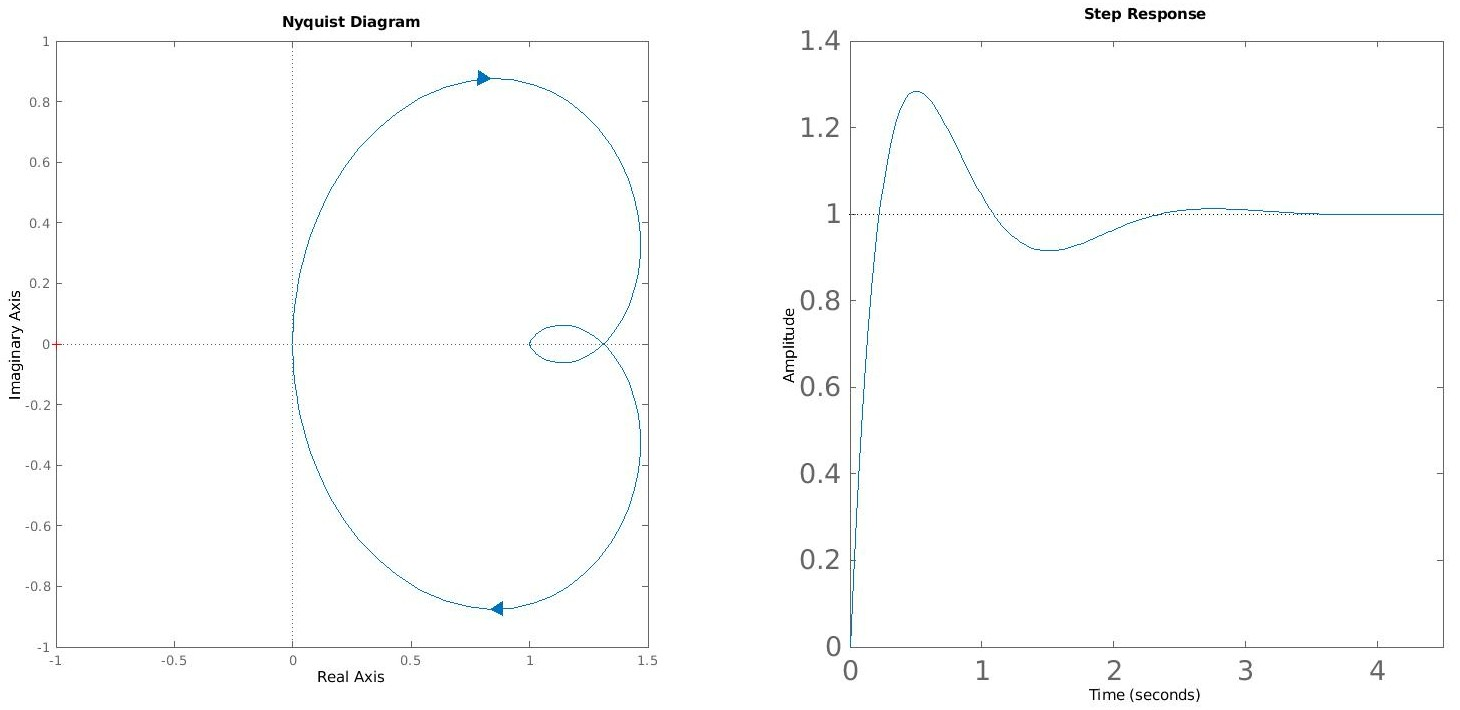
\includegraphics[width=\textwidth]{step3.jpg}
\caption{Diagramma di Nyquist e risposta allo scalino per opportune variabili del controllore PID.} \label{fig:nyquist}
\end{figure}
Una possibile scelta di queste variabili è ad esempio $K_p=3$, $K_i=1$ e $K_d=5$ che dà come risultato i grafici di figura \ref{fig:nyquist}. Si nota come in questo caso la funzione di trasferimento presenti tre poli a parte reale negativa e che il diagramma di Nyquist non circonda il punto $-1+0\cdot j$ (indicato da un punto rosso), nella figura a destra è poi indicata la risposta allo scalino del sistema, che dimostra ulteriormente le proprietà di stabilizzazione e di non polarizzazione del controllore.

% tre poli a parte reale negativa, il cui diagramma di Nyquist è rappresentato a sinistra in figura \ref{fig:nyquist}.
%Si nota come come il punto $-1+0\cdot j$ (indicato da un punto rosso) non venga circondato dal grafico, il sistema ha quindi modulo minore di uno a una fase di 180° e risulta essere stabile.

\section{Sistemi di riferimento}\label{sistemidiriferimento}
A livello di implementazione si nota come sia possibile descrivere la posizione della pallina nel piano secondo due sistemi di riferimento, il cartesiano e il polare. Questi due sono totalmente equivalenti a livello descrittivo e richiedono un controllo di due variabili tramite due PID separati rispettivamente per le variabili $(x,y)$ e $(r,\varphi)$, come descritto in figura \ref{fig:sistemiriferimento}.
\begin{figure}[h!]
\centering
\scalebox{1}{
\begin{tikzpicture}[font=\small,thick]
\draw [gray](0,2) -- (6cm,2cm);
\draw [gray](8,2) -- (14cm,2cm);
\draw  [gray](3,0) -- (3cm,4cm);
\draw  [gray,dashed](3+1.06,2) -- (3+1.06,2-1.06)node[xshift= -0.5cm,yshift= -0.3cm]{$x$};
\draw  [gray,dashed](3,2-1.06) -- (3+1.06,2-1.06)node[xshift= 0.3cm,yshift= 0.5cm]{$y$};
\draw  [gray,dashed](11,2) -- (11+1.06,2-1.06);
\draw (0,0) rectangle (6,4);
\draw (8,0) rectangle (14,4);
\draw [gray,dashed](11cm,2cm)node[xshift= 1cm,yshift= -0.4cm]{$\varphi$} -- (11.7cm,2cm) arc  (0:-45:7mm)-- cycle;
\draw [gray,dashed](11,2)node[xshift= 1cm,yshift= 0.2cm]{$r$} circle (1.5cm);
\filldraw [fill=black] (11+1.06,2-1.06) circle (5pt);
\filldraw [fill=black] (3+1.06,2-1.06) circle (5pt);
\end{tikzpicture}
}
\caption{Sistemi di riferimento cartesiano e polare.} \label{fig:sistemiriferimento}
\end{figure}
L'unica differenza sostanziale tra i due sta nell'assegnazione dei setpoint, se ad esempio si volesse assegnare una traiettoria circolare, la sua descrizione risulterebbe essere:
\begin{itemize}
\item
    $\begin{cases}
      x=cos(\tau)\\
      y=sin(\tau)\\
    \end{cases}$
 per il sistema cartesiano.
\item $\begin{cases}
      r=1\\
      \varphi=\tau\\
    \end{cases}$ per il sistema polare.
\end{itemize}
Dove $\tau$ è una variabile generica che permette alla posizione di evolvere, nel caso considerato si è scelto di associarla al tempo moltiplicato per un fattore costante opportuno che ne regola la velocità. Essendo le funzioni periodiche, all'avanzare del tempo il setpoint andrà quindi a muoversi sempre sullo stesso percorso.

Si è deciso di impiegare il sistema cartesiano per due motivi principali: 
\begin{itemize}
\item La struttura stessa della piattaforma, che va ad agire su rollio e beccheggio, influenzando direttamente le variabili $x$ e $y$.
\item La facilità di descrizione di alcune curve, come ad esempio le figure di Lissajous, che costituiscono un ottimo test per valutare le proprietà di velocità e precisione del sistema.
\end{itemize}


%Una nota particolare va fatta in merito al sistema di riferimento impiegato e di come 	questo influenzi l'operazione del controllore dal PID. I due sistemi di riferimento impiegabili sono il cartesiano e il polare, ognuno dei quali con dei rispettivi vantaggi e svantaggi. Il sistema di riferimento cartesiano richiede due PID separati per operare, uno per il controllo dell'asse $x$ e uno per il controllo dell'asse $y$, aumentando la complessità del sistema rispetto al polare che invece ne richiede solo uno. Lo svantaggio del sistema di riferimento polare si ha relativamente all'assegnazione

\section{Algoritmo di controllo}\label{algocontrollo}
Vista la versatilità di applicazione del controllore PID, l'intero problema di controllo si traduce nella determinazione della posizione della pallina sul piano e lo svolgimento di opportune equazioni per ottenere i parametri richiesti come la velocità e l'accelerazione. Questi sono impiegati rispettivamente nella componente derivativa del PID migliorato e nel filtraggio del segnale stesso. Il comportamento del sistema di controllo si può quindi riassumere nello schema a blocchi di figura \ref{fig:stabilizzazione}, dove il blocco di assegnazione dei valori alla piattaforma richiama quello di figura \ref{fig:ps}.
\begin{figure}[h!]
\centering
\scalebox{0.9}{
\begin{tikzpicture}[font=\small,thick]
 
% Start block
\node[draw,
    rounded rectangle,
    minimum width=2.5cm,
    minimum height=1cm, text width=2cm, text centered] (start) {Accensione};
    
    
% Voltage and Current Measurement
\node[draw,
    trapezium, 
    trapezium left angle = 120,
    trapezium right angle = 120,
    trapezium stretches,
    below=of block2,
    minimum width=3.5cm,
    minimum height=1cm,
    text width=3cm, text centered, below=of start
] (lettura) {Lettura posizione palla};

\node[draw,
    below=of lettura,
    minimum width=3.5cm,
    minimum height=1cm,
    text width=3cm, text centered
] (calcolo) {  Calcolo velocità e accelerazione};

\node[draw,
    below=of calcolo,
    minimum width=3.5cm,
    minimum height=1cm,
    text width=2.5cm, text centered
] (filtro) { Filtro limitando variazione};

\node[draw,
    below=of filtro,
    minimum width=3.5cm,
    minimum height=1cm,
    text width=3cm, text centered
] (pid) { PID migliorato};

\node[draw,
    diamond,
    right=of pid,
    minimum width=3.5cm,
    inner sep=2, aspect=2, xshift= 1.2cm] (acc) {Valore accettabile?};
    
\node[draw,
    trapezium, 
    trapezium left angle = 120,
    trapezium right angle = 120,
    trapezium stretches,
    below=of block2,
    minimum width=3.5cm,
    minimum height=1cm,
    text width=3cm, text centered, above=of acc, yshift= 0.5cm
] (piatt) {Assegna valore piattaforma};


\node[draw,
    right=of acc,
    minimum width=3cm,
    minimum height=1cm,
    text width=2.5cm, text centered, xshift= 1.2cm
] (max) { Usa valore massimo};
 

% Arrows
\draw 	[-latex](start) edge (lettura);		  
\draw [-latex]	(lettura) edge (calcolo);
\draw [-latex]	(calcolo) edge (filtro);	
\draw [-latex]	(filtro) edge (pid);
\draw [-latex]	(pid) edge (acc);
\draw [-latex]	(acc) edge (max)node[fill=white,inner sep=2,xshift = 2.5cm]{No};
\draw [-latex]	(max) |- (piatt);
\draw [-latex]	(acc) edge (piatt) node[fill=white,inner sep=2, yshift=1.5cm]{Sì};
\draw [-latex]	(piatt) |- (lettura);


\end{tikzpicture}
}
\caption{Schema logico sistema di stabilizzazione.} \label{fig:stabilizzazione}
\end{figure}
\newpage

\chapter{Realizzazione pratica}\label{realizzazionepratica}
La realizzazione pratica del progetto è stata un processo discretamente complesso, eseguito in modo sequenziale e analizzando costantemente le varie criticità. Questo si è svolto principalmente in 3 fasi: l'assemblaggio, la programmazione e la taratura del sistema, rispettivamente descritte in dettaglio nelle sezioni \ref{assemblaggio}, \ref{programmazione} e \ref{taratura}.

\section{Assemblaggio}\label{assemblaggio}
Sono state fornite la base con i servomotori, la piattaforma ed i relativi braccetti di collegamento, il piano resistivo e la scheda Arduino UNO dotata di shield. I primi dubbi si sono verificati durante l'assemblaggio in quanto esistono quattro possibili varianti di piattaforma di Stewart con attuatori rotativi, rispettivamente con le manovelle interne o esterne e con i braccetti collegati alla piattaforma sullo stesso lato o su lati opposti. Analizzando la piattaforma si è preferito optare per una disposizione con manovelle esterne e braccetti su lati opposti. Si nota come queste configurazioni siano completamente equivalenti a livello matematico e necessitano unicamente di un ricalcolo della posizione dei punti di aggancio della piattaforma, il che mostra l'adattabilità del modello stesso. Alcuni dei pezzi necessari al completamento dell'assemblaggio, come gli agganci per la piattaforma e il piano resistivo, erano mancanti e dovevano essere realizzati. Disponendo di una stampante 3D si è optato per stampare i pezzi in modo da permettere una prototipazione rapida. Non disponendo dei file relativi alle dimensioni della base e della piattaforma, di compensato tagliato al laser, è stato fondamentale ricostruire fedelmente il modello in ambiente CAD per poi procedere alla modellazione delle parti mancanti (figura \ref{fig:renderstewart}). 
\begin{figure}[h!]
\centering
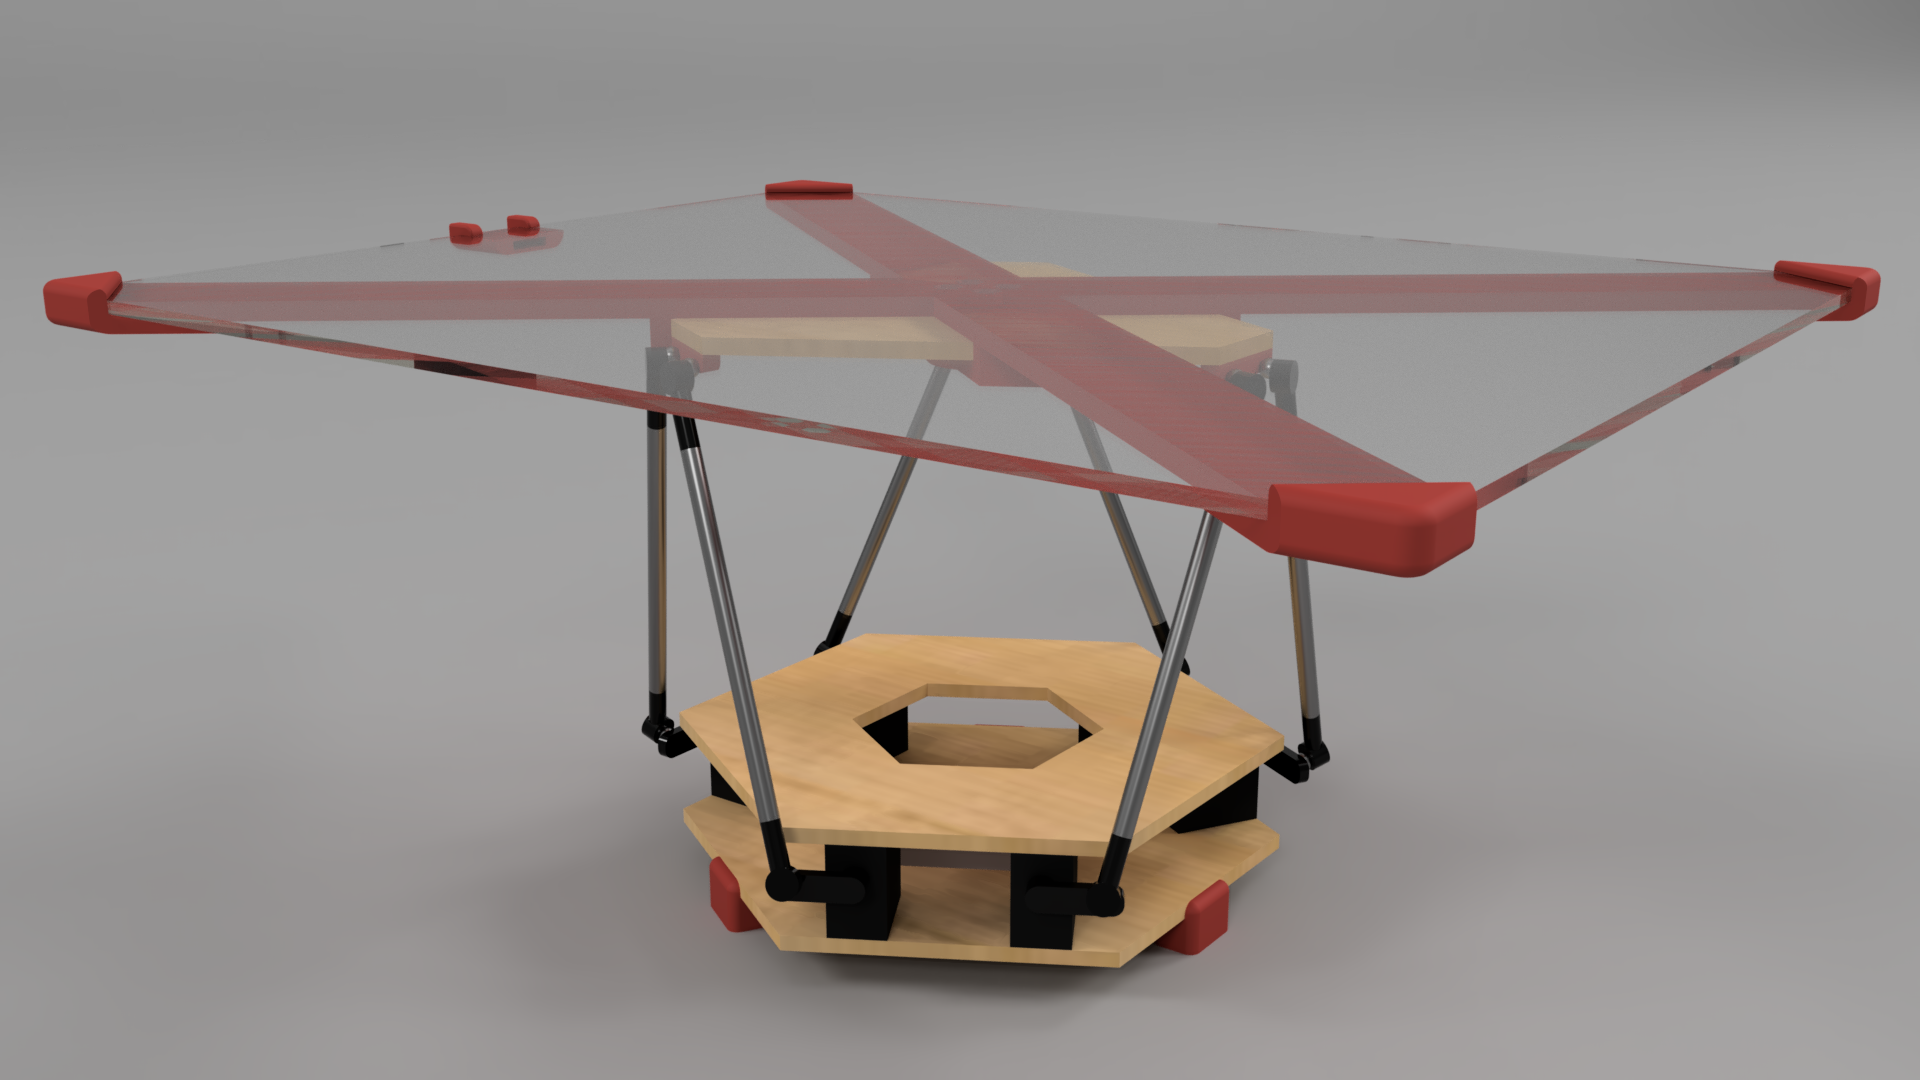
\includegraphics[width=\textwidth]{stewart.png}
\caption{Modello 3D della piattaforma di Gough-Stewart realizzata.} \label{fig:renderstewart}
\end{figure}
I modelli sono stati realizzati con il software Fusion360 e stampati in materiale plastico PLA con infill a nido d'ape per avere un buon compromesso tra leggerezza e rigidità. Ultimata la costruzione si è rivolta l'attenzione alle componenti elettroniche, innanzitutto è stato realizzato un connettore apposito per permettere un collegamento stabile tra i servomotori e la scheda Arduino, evitando inoltre possibili intralci al movimento della piattaforma. Notando la fragilità delle uscite del digitalizzatore, tramite un flat-cable flessibile, si è preferito realizzare un apposito aggancio che serva innanzitutto da strain-relief e faciliti la connessione dei cavi dupont per interfacciarsi con Arduino. Come precedentemente esposto nella sezione \ref{hbridge}, in seguito ad un'analisi tramite multimetro della resistenza del digitalizzatore si è notato che un controllo diretto richiamerebbe solo $2V$, più che dimezzando la risoluzione del piano rispetto ai $5V$ nominali. La realizzazione pratica del driver per il piano resistivo ha richiesto l'impiego di un montaggio apposito su basetta di vetronite per ridurre al minimo le capacità parassite e i falsi contatti rispetto ad una basetta sperimentale. 
%Non essendo certi dell'influenza dello shoot-through dei MOSFET è stata prevista una resistenza di $1\Omega$ verso massa, in modo da limitare l'eventuale corrente massima a $5A$, entro il range previsto dal datasheet di $4A$ continui e $27A$ pulsati. Un altra caratteristica è la presenza delle resistenze di Gate, queste sono state previste nel caso in cui si dovesse eseguire un ulteriore pilotaggio tramite componente attivo per evitare lo shoot-through ma in seguito alla prova pratica questo non è stato necessario. 
Si è quindi svolta un'analisi dei tempi di commutazione con l'oscilloscopio, importantissima nella successiva parte di programmazione, con la quale si è determinato il periodo minimo di campionamento che risulta essere di soli $50\mu s$. Infine è stato implementato senza particolari accorgimenti il joystick in quanto è bastato collegare i cavi direttamente allo shield per avere delle ottime letture.
\newpage
\section{Programmazione}\label{programmazione}
La programmazione è senza dubbio la parte principale del progetto e per la sua versatilità ricopre un ruolo fondamentale. Vista la complessità del sistema, lo sviluppo del software è stato diviso in diversi blocchi operativi, ognuno dei quali svolge un ruolo diverso e indipendente dagli altri, che saranno trattati nelle successive sezioni.
%\begin{itemize}
%\item Il controllo della piattaforma di Stewart.
%\item La lettura e il filtraggio dei dati in ingresso dal piano resistivo.
%\item L'elaborazione del segnale in ingresso da parte del PID.
%\item La gestione dei comandi assegnati tramite joystick.
%\end{itemize}
%Segue un analisi di queste procedure.
\subsection{Controllo della piattaforma di Stewart}
Il controllo della piattaforma di Stewart è stato trattato in modo estensivo dal punto di vista matematico nel capitolo \ref{pianostewart}, la programmazione in questo caso si occupa quindi di riproporre fedelmente queste equazioni in linguaggio \texttt{C}, con alcuni accorgimenti specifici relativi all'implementazione del software stesso. Come struttura dati, visto il numero elevato di variabili, si è scelto di impiegare le matrici, vista anche la facilità di implementazione di algoritmi per eseguire le varie operazioni richieste. 
L'assegnazione della posizione alla piattaforma di Stewart è svolta richiamando la seguente funzione e fornendo in ingresso i sei parametri richiesti per definire univocamente la posizione del piano nello spazio.
\begin{minted}[frame=lines,framesep=2mm,baselinestretch=1.2,bgcolor=LightGray,fontsize=\footnotesize,linenos]{C}
setPosition(x, y, z, rol, pit, yaw);
\end{minted}
Una nota particolare va fatta in merito all'algoritmo di controllo delle posizioni irraggiungibili presente nel seguente listato.
\begin{minted}[frame=lines,framesep=2mm,baselinestretch=1.2,bgcolor=LightGray,fontsize=\footnotesize,linenos]{C}
int emergenza = 0;
  for(int i = 0; i < 6; i++){
    if(constrain(getAmpImp(alfa[i],i),inf,sup) == sup ||
       constrain(getAmpImp(alfa[i],i),inf,sup) == inf ||
       isnan(constrain(getAmpImp(alfa[i],i),inf,sup))){     
      emergenza++;
    }
  }
  if(emergenza == 0){
    for(int i = 0; i < 6; i++){
        servo[i].writeMicroseconds(constrain(getAmpImp(alfa[i],i),inf,sup));
    }
  }
  else{
    Serial.println("Limite raggiunto, arresto motori.");
    fermoEmergenza();
  }
\end{minted}
Ogni computazione della posizione richiesta comporta la generazione di sei valori che saranno poi assegnati come angoli ai servomotori. Prima che questo avvenga, un ciclo \texttt{for} si occupa di controllare tutti i valori generati per verificare che questi siano compresi in un limite inferiore e superiore, ma soprattutto verifica che il valore sia effettivamente computabile. Nella formula \eqref{alfa} infatti, nel caso sia assegnato un valore impossibile alla funzione $arcsin$, questa diventa indefinita, espressa in \texttt{C} con il simbolo \texttt{NaN}\footnote{Not A Number.}, è per questo fondamentale l'impiego della funzione \texttt{isnan} per verificare se questo è il caso. Se una delle tre condizioni non è rispettata il contatore \texttt{emergenza} viene incrementato, utile per capire quanti servomotori abbiano ricevuto un valore errato. A questo punto, se non si sono verificati disguidi, si può procedere con l'assegnazione dei valori impiegando la funzione \texttt{writeMicroseconds}, che assegna l'angolo ai servomotori dopo che questo è stato opportunamente convertito in microsecondi dalla funzione \texttt{getAmpImp}.
Se uno degli angoli non rispetta i vincoli l'assegnazione viene saltata e si passa direttamente alla routine di blocco \texttt{fermoEmergenza} che blocca il sistema e accende un LED lampeggiante di segnalazione.

\subsection{Lettura e filtraggio dati ottenuti dal piano resistivo}
La lettura dei segnali provenienti dal piano resistivo è svolta leggendo sequenzialmente lo stato del pin analogico di Arduino con la seguente funzione:
\begin{minted}[frame=lines,framesep=2mm,baselinestretch=1.2,bgcolor=LightGray,fontsize=\footnotesize,linenos]{C}
void getSense(){
  digitalWrite(in1,HIGH);
  digitalWrite(in2,LOW);
  delayMicroseconds(on);
  x = (analogRead(sensePin)-100)*(0.34/820);

  digitalWrite(in1,LOW);
  digitalWrite(in2,HIGH);
  delayMicroseconds(on);
  y = (analogRead(sensePin)-100)*(0.27/820);
  lastsense = micros();
}
\end{minted}
Questa prevede la creazione di un gradiente lungo l'asse $x$, per la durata espressa dalla variabile \texttt{on} che permette la stabilizzazione del segnale, la cui durata è ricavata sperimentalmente osservando il tempo di stabilizzazione del segnale all'oscilloscopio come riportato in figura \ref{fig:osc2}, che risulta essere di circa $10\mu s$ a causa della gobba negativa, dovuta allo shoot-through durante la commutazione dei MOSFET. Si nota come questo tempo sia stato esteso a $50 \mu s$ per essere sicuri di evitare ogni tipo di disturbo.
\begin{figure}[h!]
\centering
\begin{subfigure}{0.48\textwidth}
    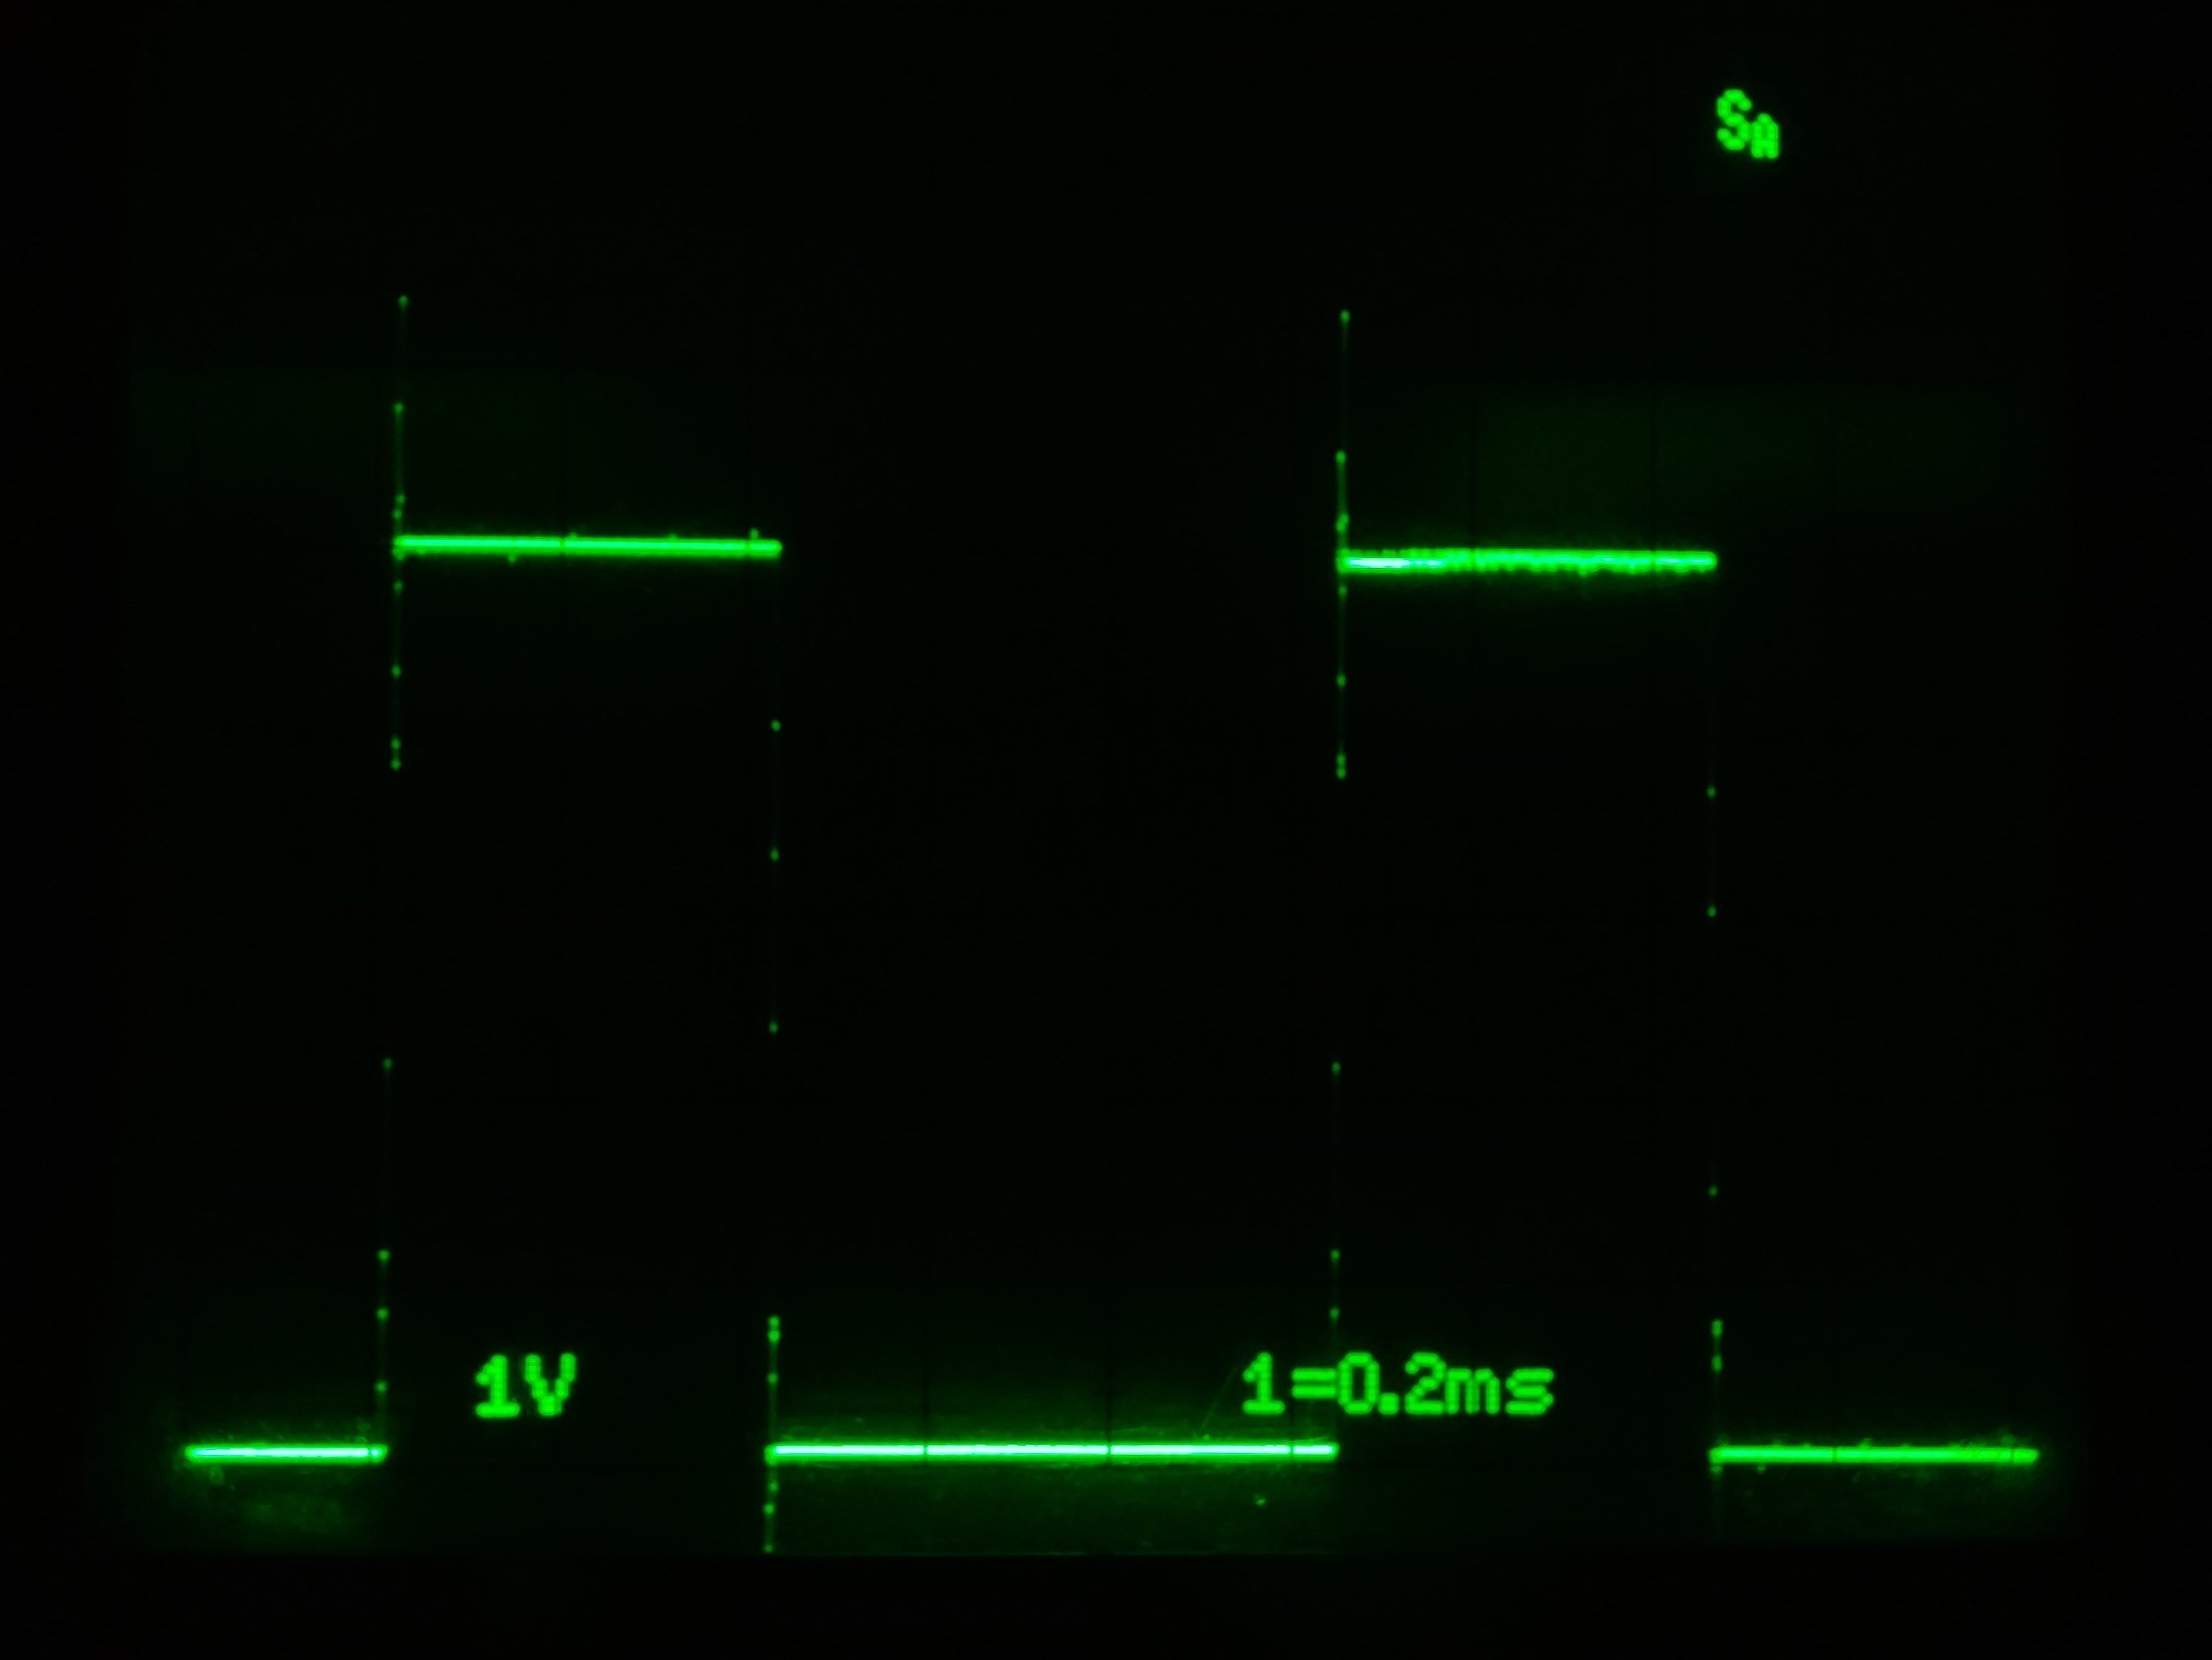
\includegraphics[width=\textwidth]{osc1.jpg}
    \caption{Periodo del segnale di controllo.}
    \label{fig:osc1}
\end{subfigure}
\hfill
\begin{subfigure}{0.48\textwidth}
    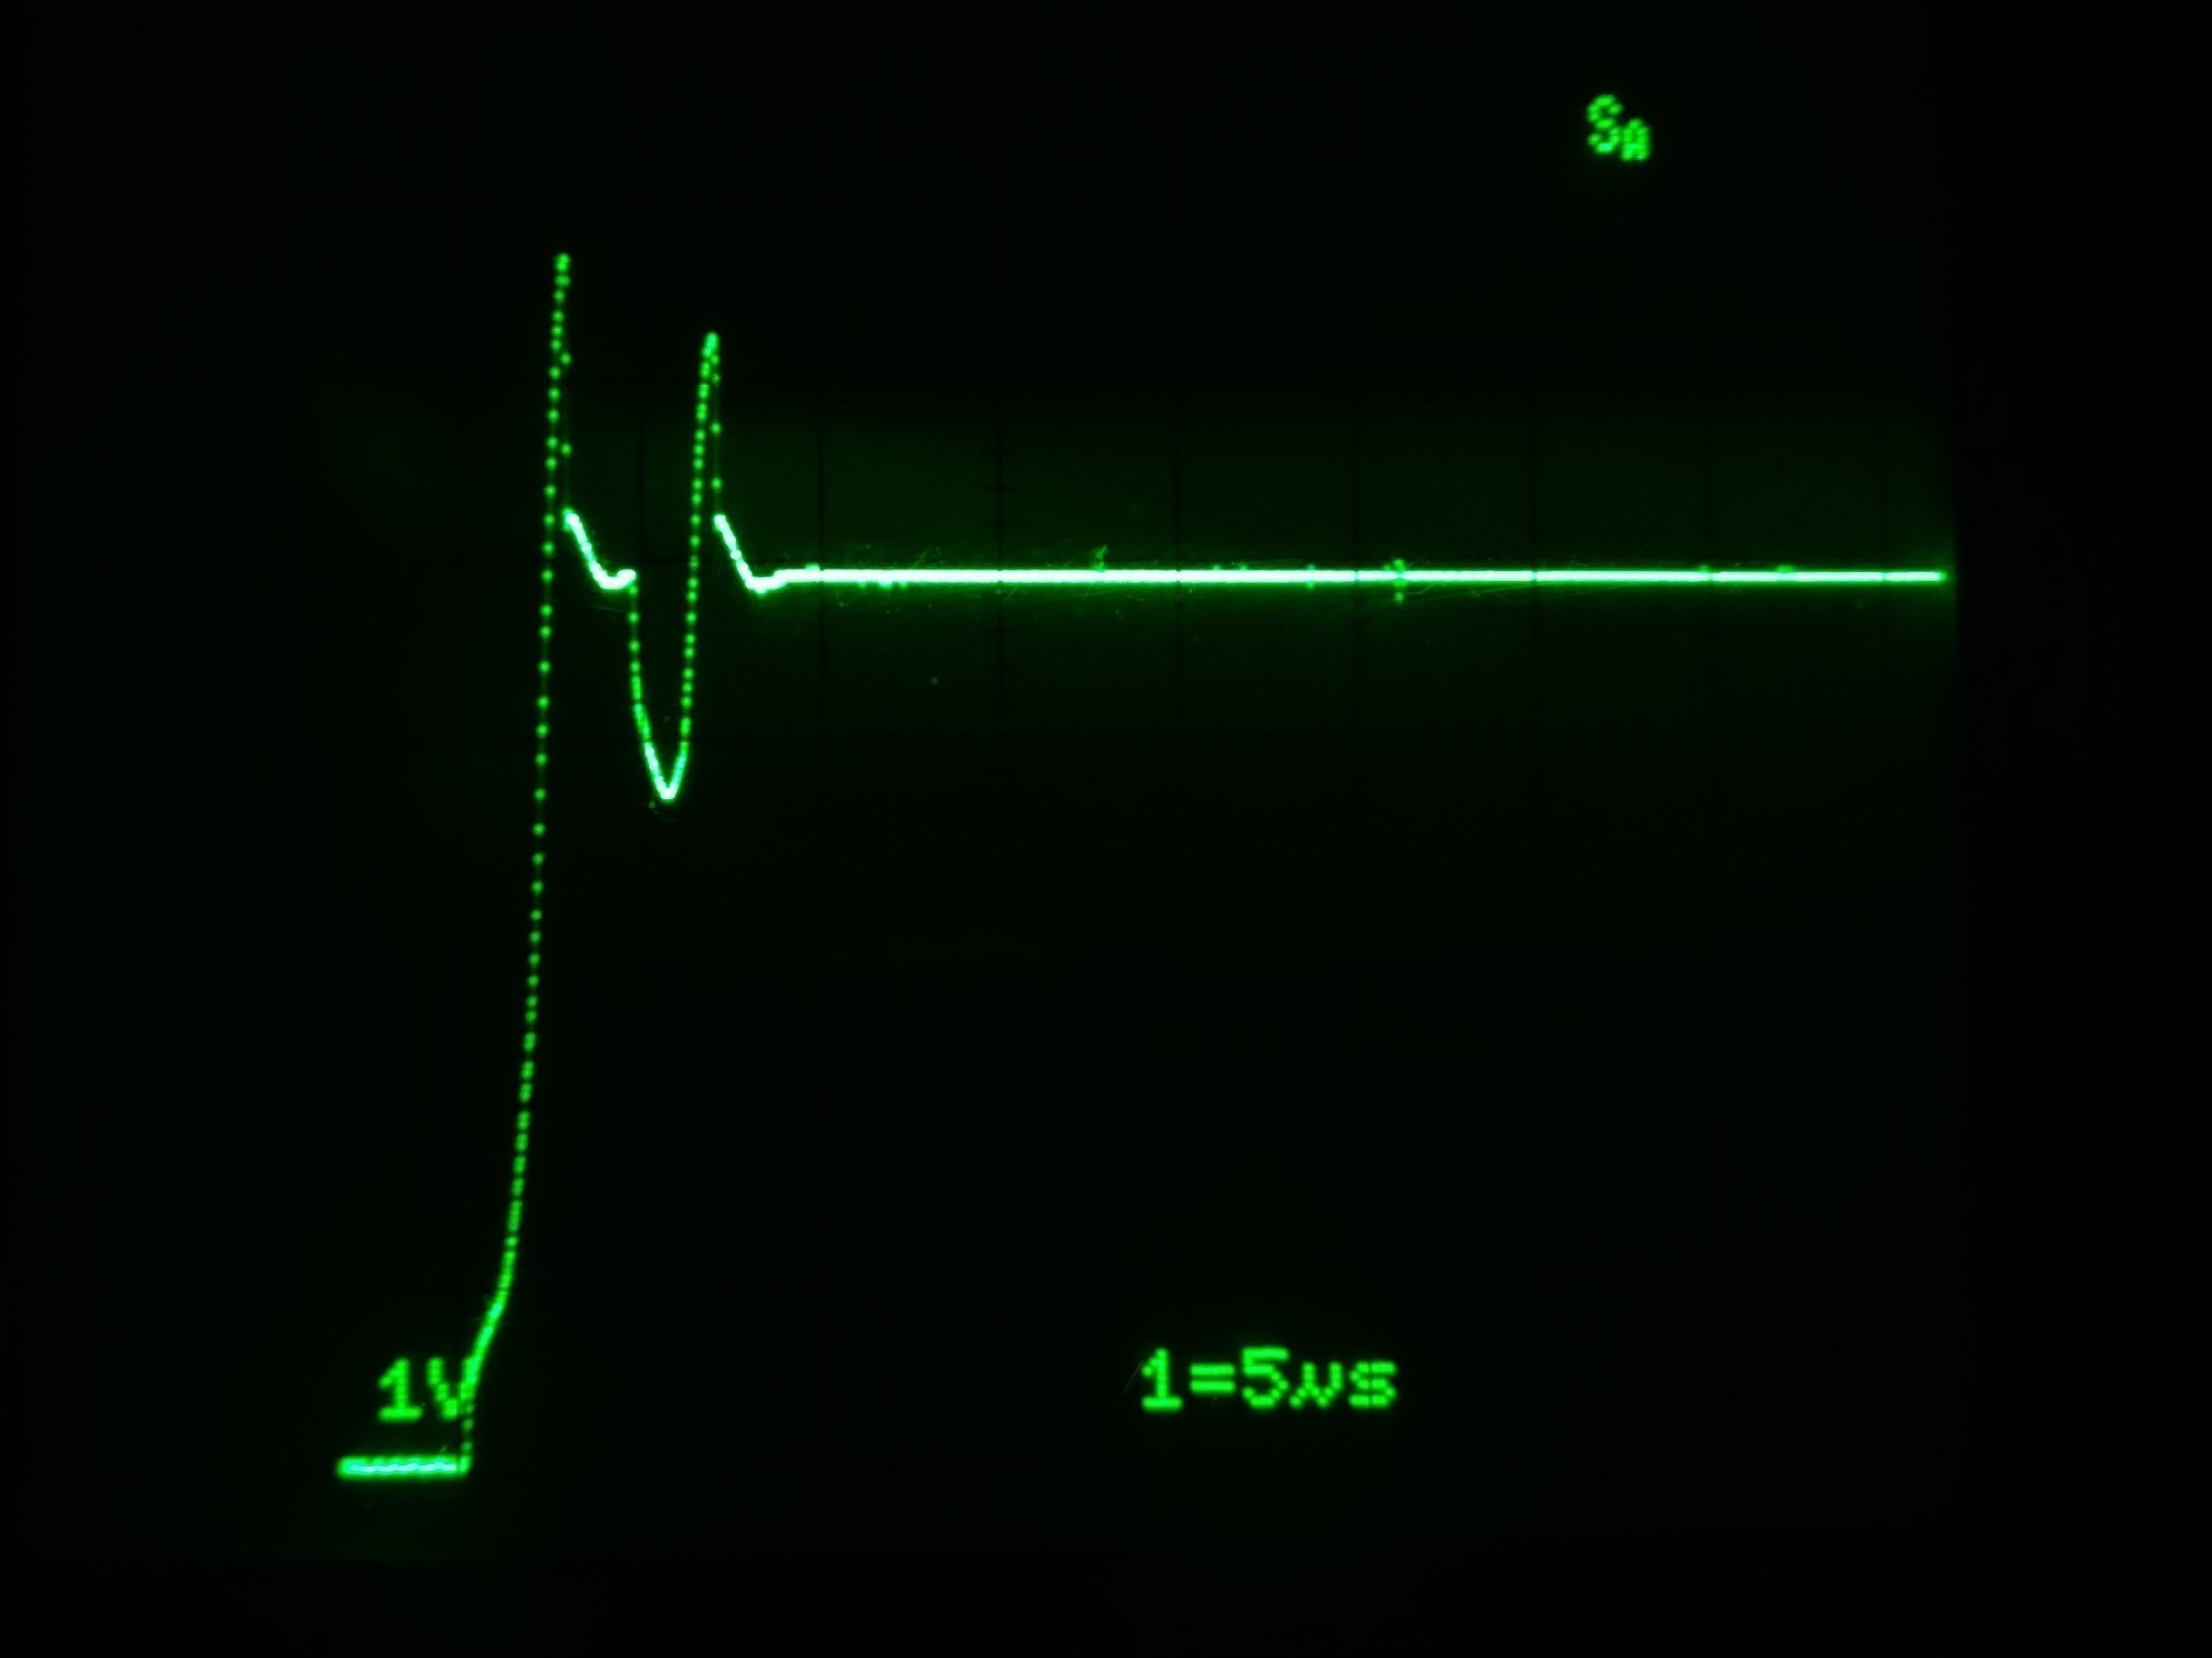
\includegraphics[width=\textwidth]{osc2.jpg}
    \caption{Fronte di salita del segnale di controllo.}
    \label{fig:osc2}
\end{subfigure}
\hfill
\end{figure}
In seguito alla stabilizzazione si procede con il campionamento. Lo stesso procedimento si ripeterà in modo del tutto analogo per l'asse $y$. Si nota come il tempo di ciclo indicato in figura \ref{fig:osc1} sia di $1 ms$, questo comprende tutte le operazioni di misura e calcolo richieste dall'algoritmo di controllo. Viene inoltre effettuata una semplice conversione della posizione da step a metri prima di assegnarla alla variabile. L'elemento chiave per un buon funzionamento del controllore è l'impiego di dati liberi da rumore e impulsi esterni, ciò detto, i dati provenienti dal piano resistivo si sono però subito mostrati non ideali, presentando un rumore impulsivo estremamente elevato, di ampiezza pari al 50\% della massima escursione del segnale utile. Questi impulsi sono principalmente dovuti alla presenza di una lieve zigrinatura sul digitalizzatore resistivo, probabilmente dovuta ai distanziatori tra i due strati conduttivi, che dà alla pallina un moto non del tutto uniforme ma con dei piccoli sobbalzi che ne fanno perdere il contatto. Per evitare questo effetto si è provato a sovrapporre al piano uno strato di materiale liscio, che colmasse le asperità, ma questo si è rivelato di scarso successo. Vista la necessità di inserire un filtraggio si è preferita un implementazione software rispetto ad una hardware per avere una maggiore flessibilità. Il filtraggio scelto non può comportare un ritardo eccessivo nel tempo di risposta, si è quindi optato per un filtro costituito da due parti, una lineare e una non lineare, opportunamente pesate per migliorare il segnale. La parte lineare è costituita da una media, su un numero variabile di valori, con lo scopo di ridurre l'effetto dei disturbi casuali mentre la parte non lineare opera da filtro passa basso, limitando la massima escursione del segnale tra un campionamento e il successivo con lo scopo di eliminare il rumore impulsivo. Per eliminare il rumore impulsivo si sarebbe anche potuto impiegare un filtro mediano ma vista la peculiarità del disturbo, che colpisce un numero variabile di campioni, questo non sarebbe stato d'aiuto. Nel seguente listato è indicato il processo di filtraggio passa basso della posizione della pallina nel piano.
\begin{minted}[frame=lines,framesep=2mm,baselinestretch=1.2,bgcolor=LightGray,fontsize=\footnotesize,linenos]{C}
xVel = (x - xOld)/deltaTime;
yVel = (y - yOld)/deltaTime;

float maxVel = 0.4;
if(abs(xVel) > maxVel){
  if(xVel > 0){
    x = xOld + maxVel*(deltaTime);
  }
  else{
    x = xOld - maxVel*(deltaTime);
  }
}
if(abs(yVel) > maxVel){
  if(yVel > 0){
    y = yOld + maxVel*(deltaTime);
  }
  else{
    y = yOld - maxVel*(deltaTime);
  }
}
\end{minted}
In questo caso la derivata della posizione è la velocità, calcolata rispetto alla posizione precedente e al tempo di ciclo. Si è quindi imposta una velocità massima, che limita la pendenza del grafico della posizione, eliminando così in modo efficace gli impulsi più sostanziali come visibile in figura \ref{fig:filtraggioposizione}, dove la linea verde indica il segnale originale e la rossa quello ottenuto in seguito al filtraggio.
\begin{figure}[h!]
\centering
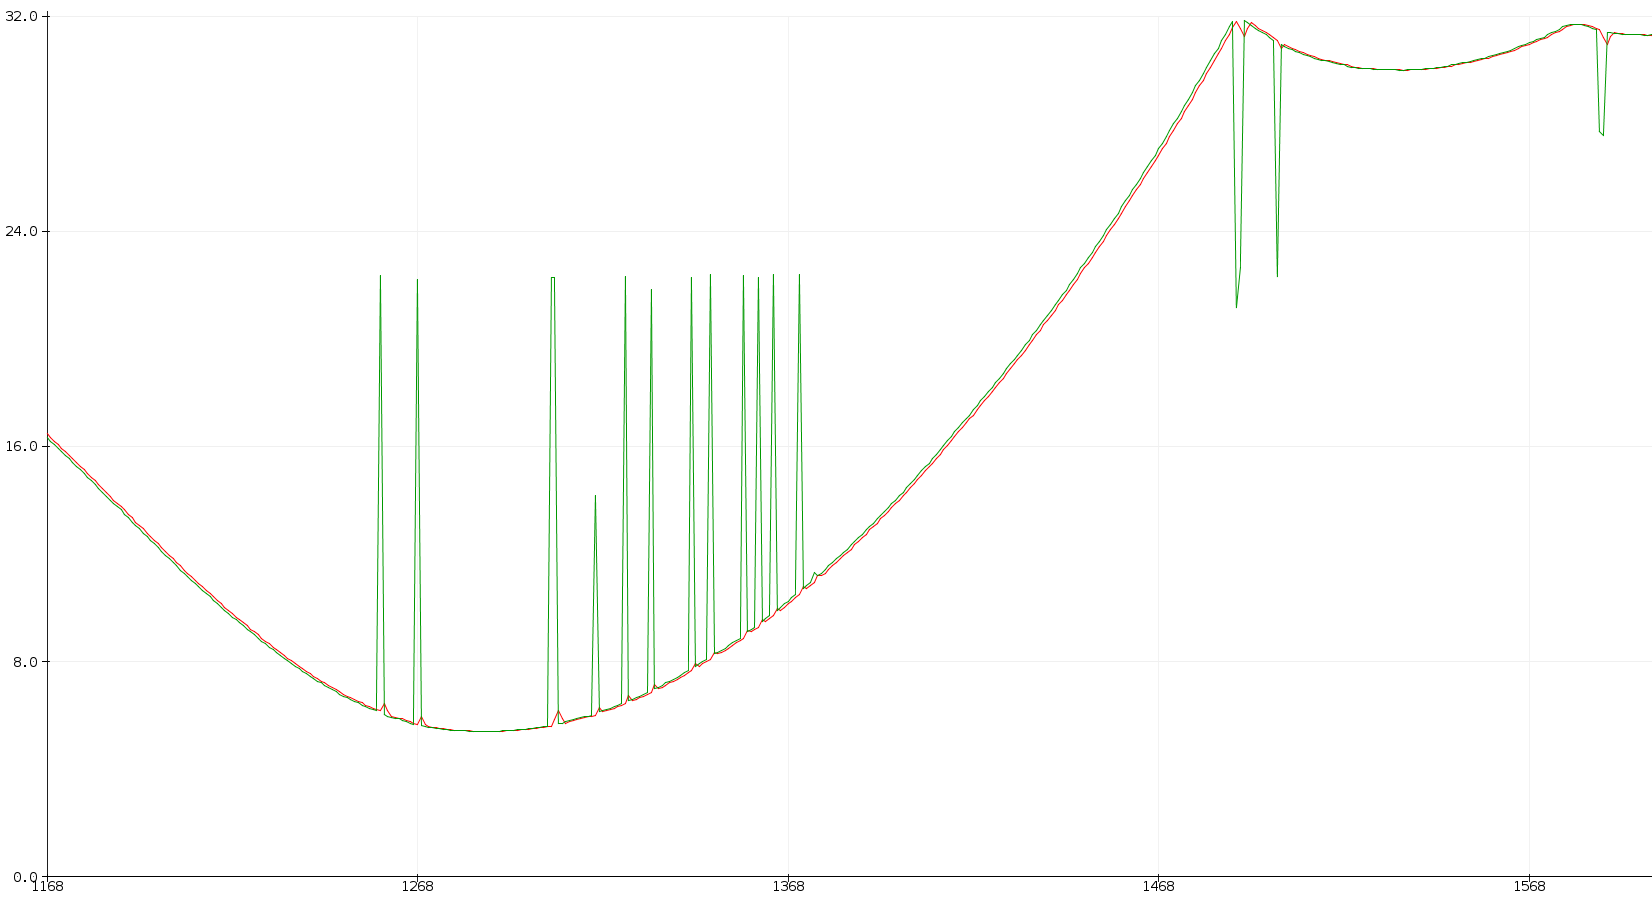
\includegraphics[width=\textwidth]{filtraggio2.png}
\caption{Confronto diretto tra segnale in ingresso e filtrato.} \label{fig:filtraggioposizione}
\end{figure}
Si nota poi che svolgendo la derivata del segnale filtrato, questa tenderà ad amplificare il piccolo rumore residuo come già precedentemente discusso nella sezione \ref{betterpid}, si è quindi deciso di ripetere un operazione di filtraggio analoga per la velocità limitando questa volta l'accelerazione massima.
\subsection{Controllore PID}
Il codice del controllore PID si occupa di implementare in \texttt{C} le operazioni descritte nel capitolo \ref{controllopalla} ed in particolare il diagramma in figura \ref{fig:pidmigliorato}.
Si nota in particolare come il PID a tutti gli effetti controlli solo due delle sei variabili della piattaforma, rollio e beccheggio, in quanto sufficienti a garantire la stabilizzazione della palla, mentre le altre variabili sono scelte costanti per semplicità.
Questo si nota immediatamente osservando il comando di assegnazione della posizione presente nel seguente listato.
\begin{minted}[frame=lines,framesep=2mm,baselinestretch=1.2,bgcolor=LightGray,fontsize=\footnotesize,linenos]{C}
setPosition(0,0,108,radians(tiltX),radians(tiltY),radians(0));
\end{minted}
In questo caso le coordinate $x$ e $y$ sono fissate al centro, l'altezza di riferimento è scelta a $108mm$ rispetto alla base per garantire un buon range di movimento, il rollio e il beccheggio sono impartiti dal PID con le variabili \texttt{tiltX},  \texttt{tiltY} e infine l'imbardata è bloccata a $0^\circ$.

\subsection{Assegnazione dei comandi}\label{assegnazionecomandi}
L'assegnazione dei comandi è svolta tramite l'ausilio di un joystick analogico, la presenza di uno switch interno ha inoltre permesso di disporre i comandi su diversi livelli. Nel livello base sono programmate delle analisi statiche, ovvero con un setpoint fisso, il joystick centrato imposta il setpoint al centro del piano, le altre 4 direzioni (joystick in alto, basso, sinistra, destra) hanno lo scopo di spostare il setpoint nella rispettiva direzione di $6cm$. Questi setpoint sono ottimi per valutare la risposta al gradino del sistema che sarà poi fondamentale nella sezione relativa alla taratura. Il secondo livello, raggiungibile premendo l'interruttore, offre la possibilità di eseguire delle analisi dinamiche, in queste il setpoint è in costante movimento e sono utili per mostrare la responsività e la precisione del sistema. Queste analisi dinamiche si incentrano sulla realizzazione di curve di vario tipo da parte della pallina, ottenibili come figure di Lissajous variando il rapporto tra le frequenze e la fase di due segnali sinusoidali assegnati rispettivamente agli assi $x$ e $y$, come in figura \ref{fig:lissajous}. Si nota come sono stati mantenuti rapporti di frequenza relativamente bassi, principalmente per evitare figure troppo complesse e di difficile valutazione.
\begin{figure}[h!]
\centering
\begin{subfigure}{0.48\textwidth}
    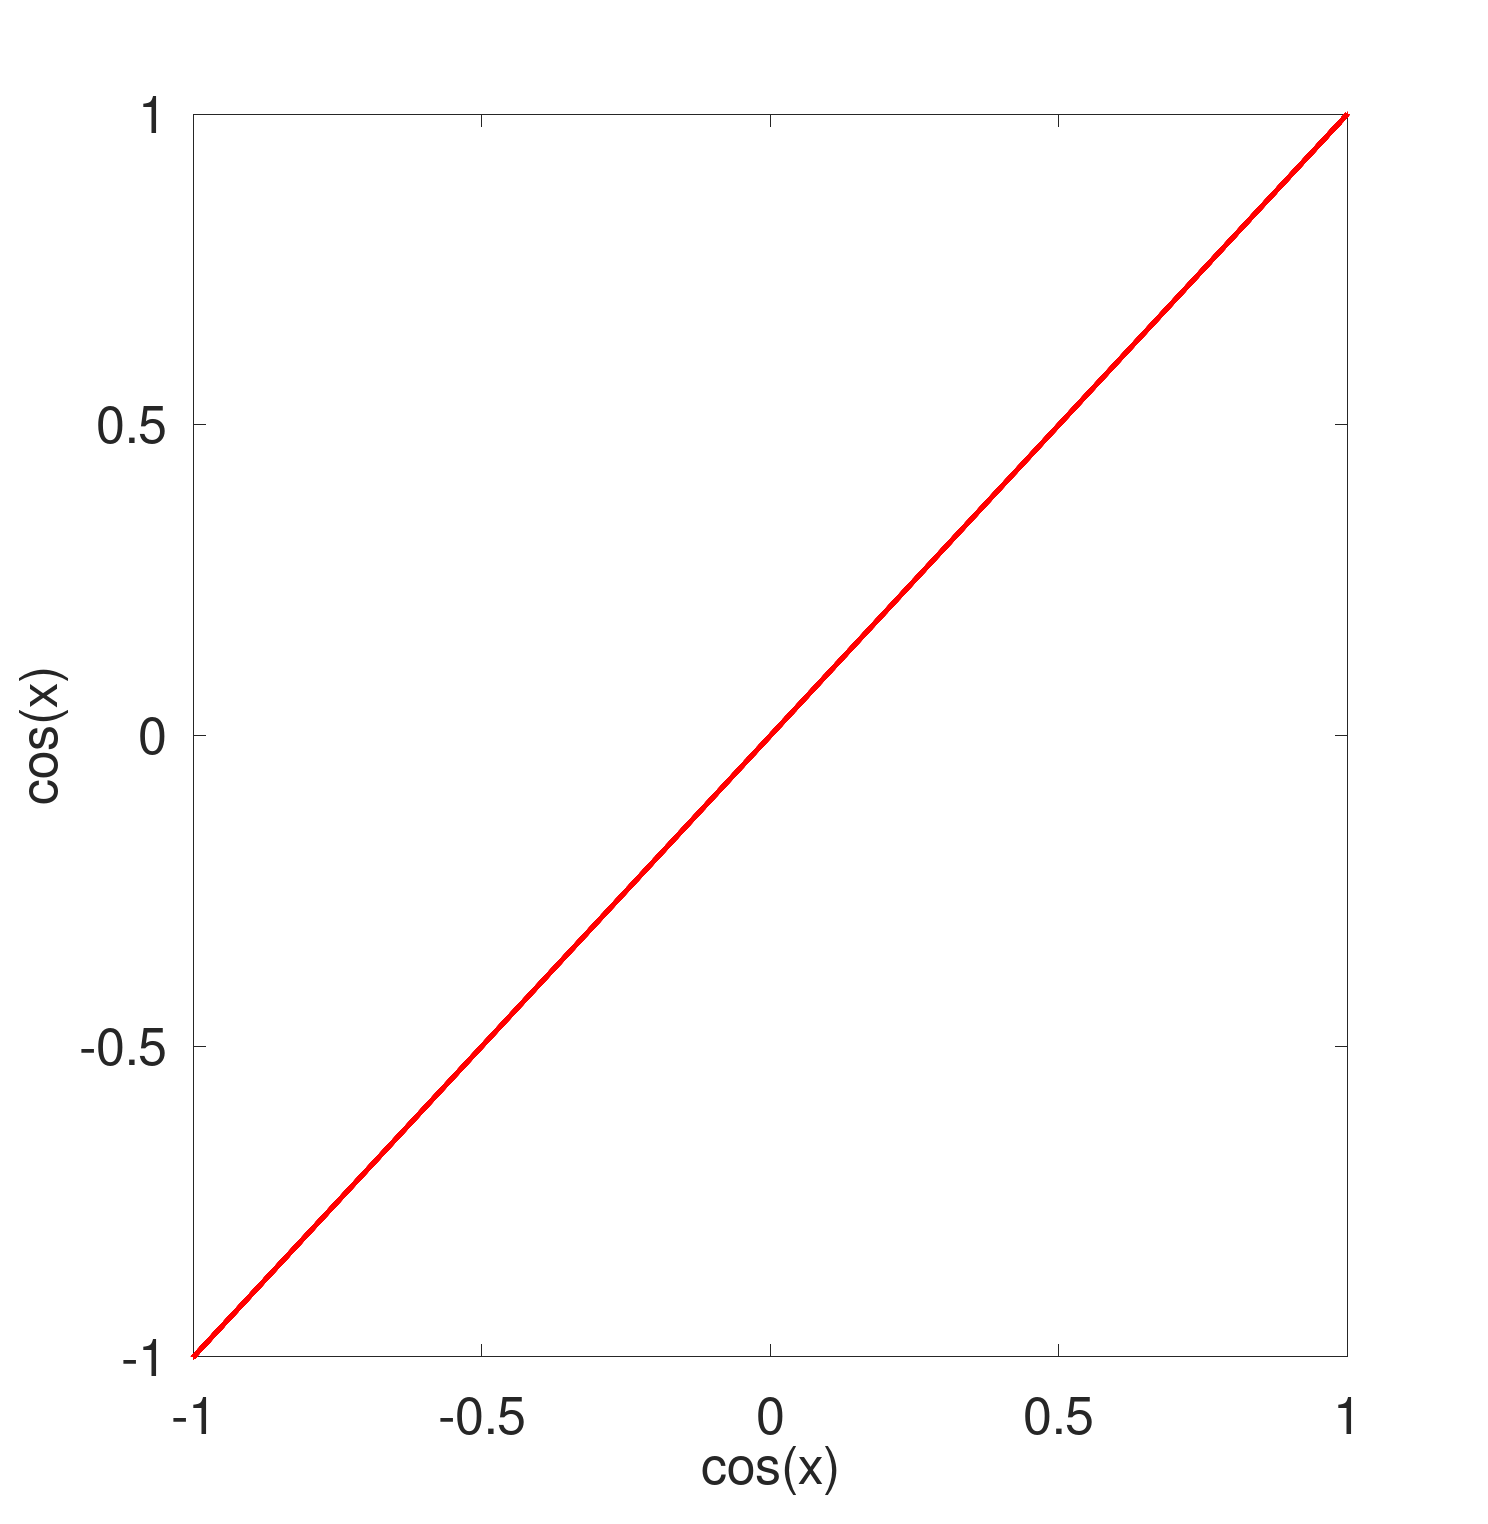
\includegraphics[width=\textwidth]{lissajous1.png}
    \caption{Frequenza 1:1, $\Delta \phi= 0$.}
    \label{fig:second}
\end{subfigure}
\hfill
\begin{subfigure}{0.48\textwidth}
    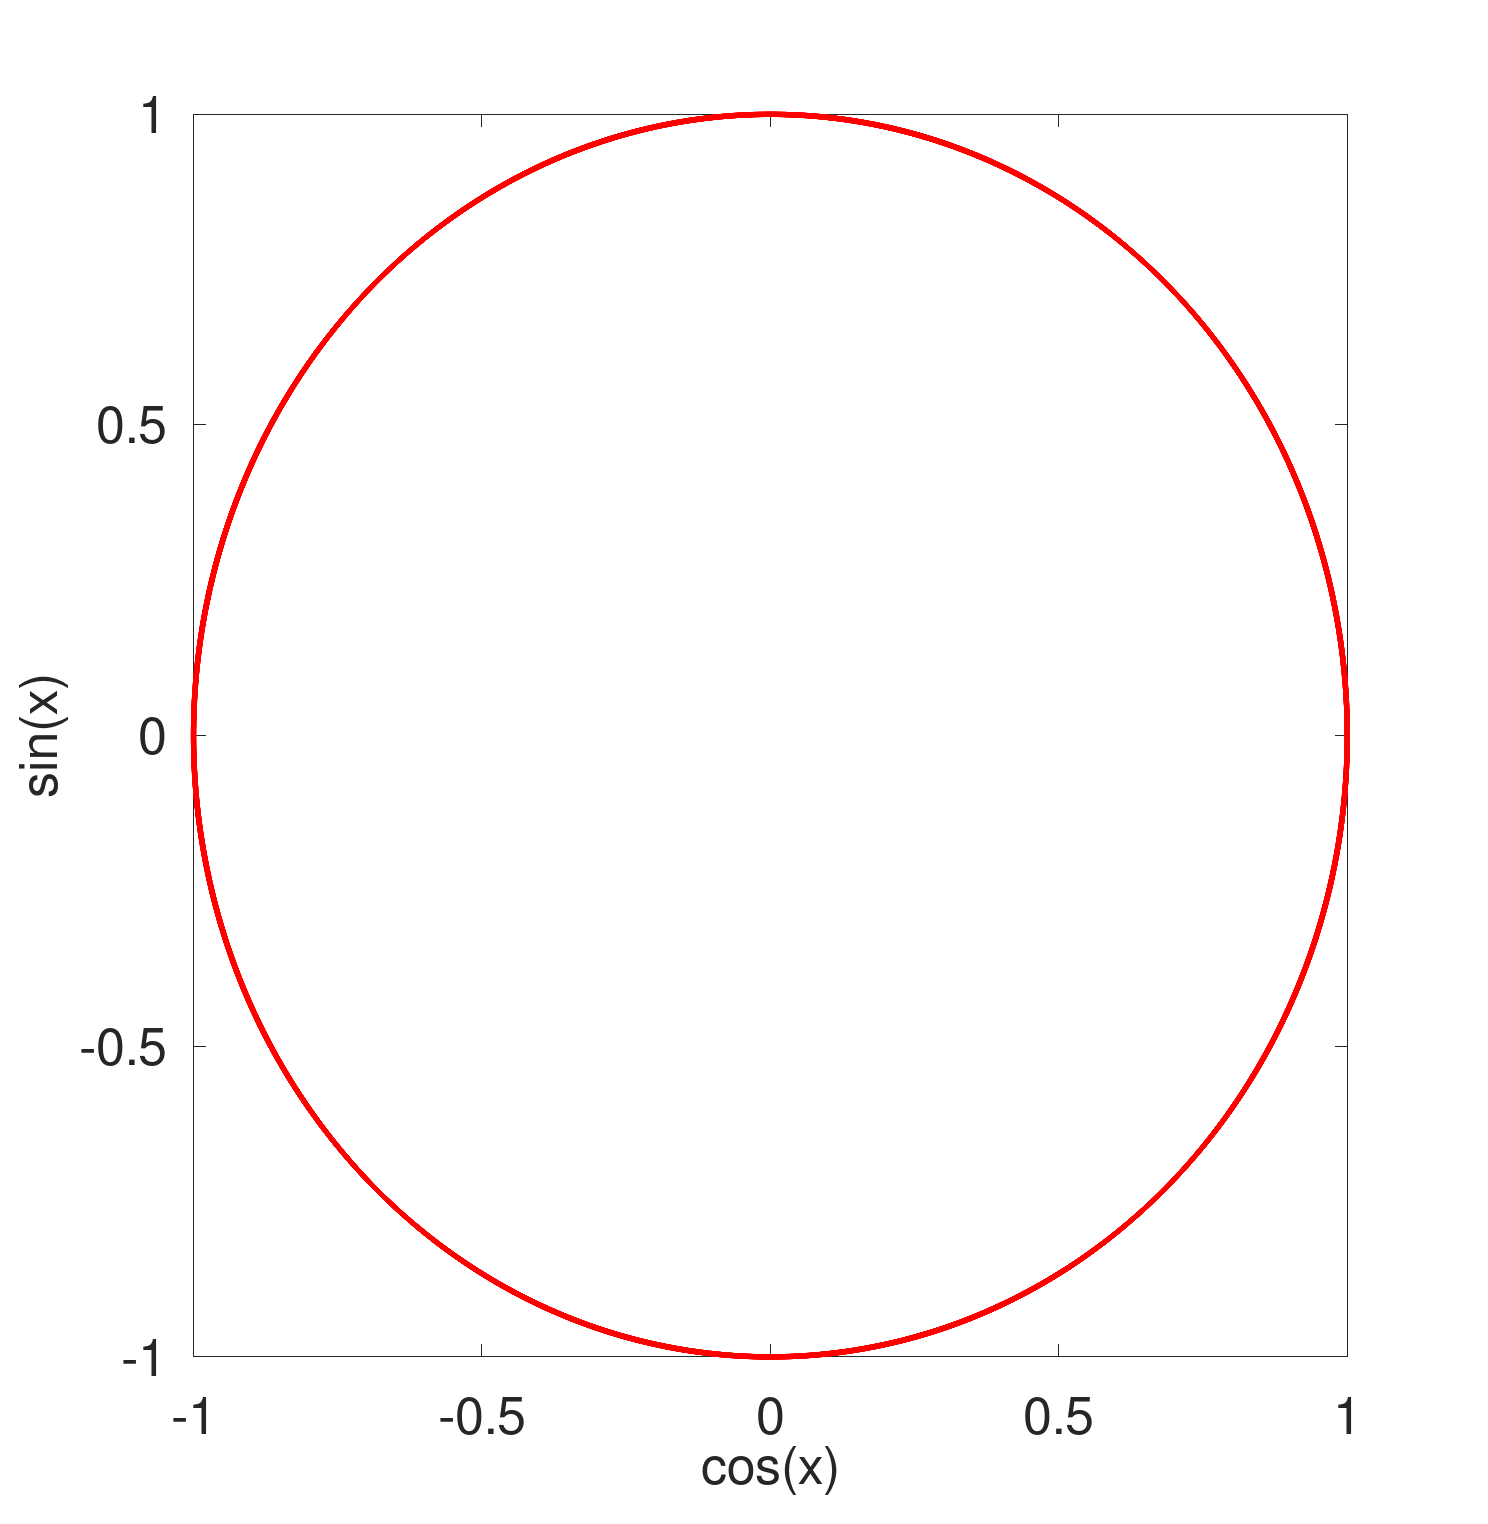
\includegraphics[width=\textwidth]{lissajous2.png}
    \caption{Frequenza 1:1, $\Delta \phi= \frac{\pi}{2}$.}
    \label{fig:third}
\end{subfigure}
\hfill
\begin{subfigure}{0.48\textwidth}
    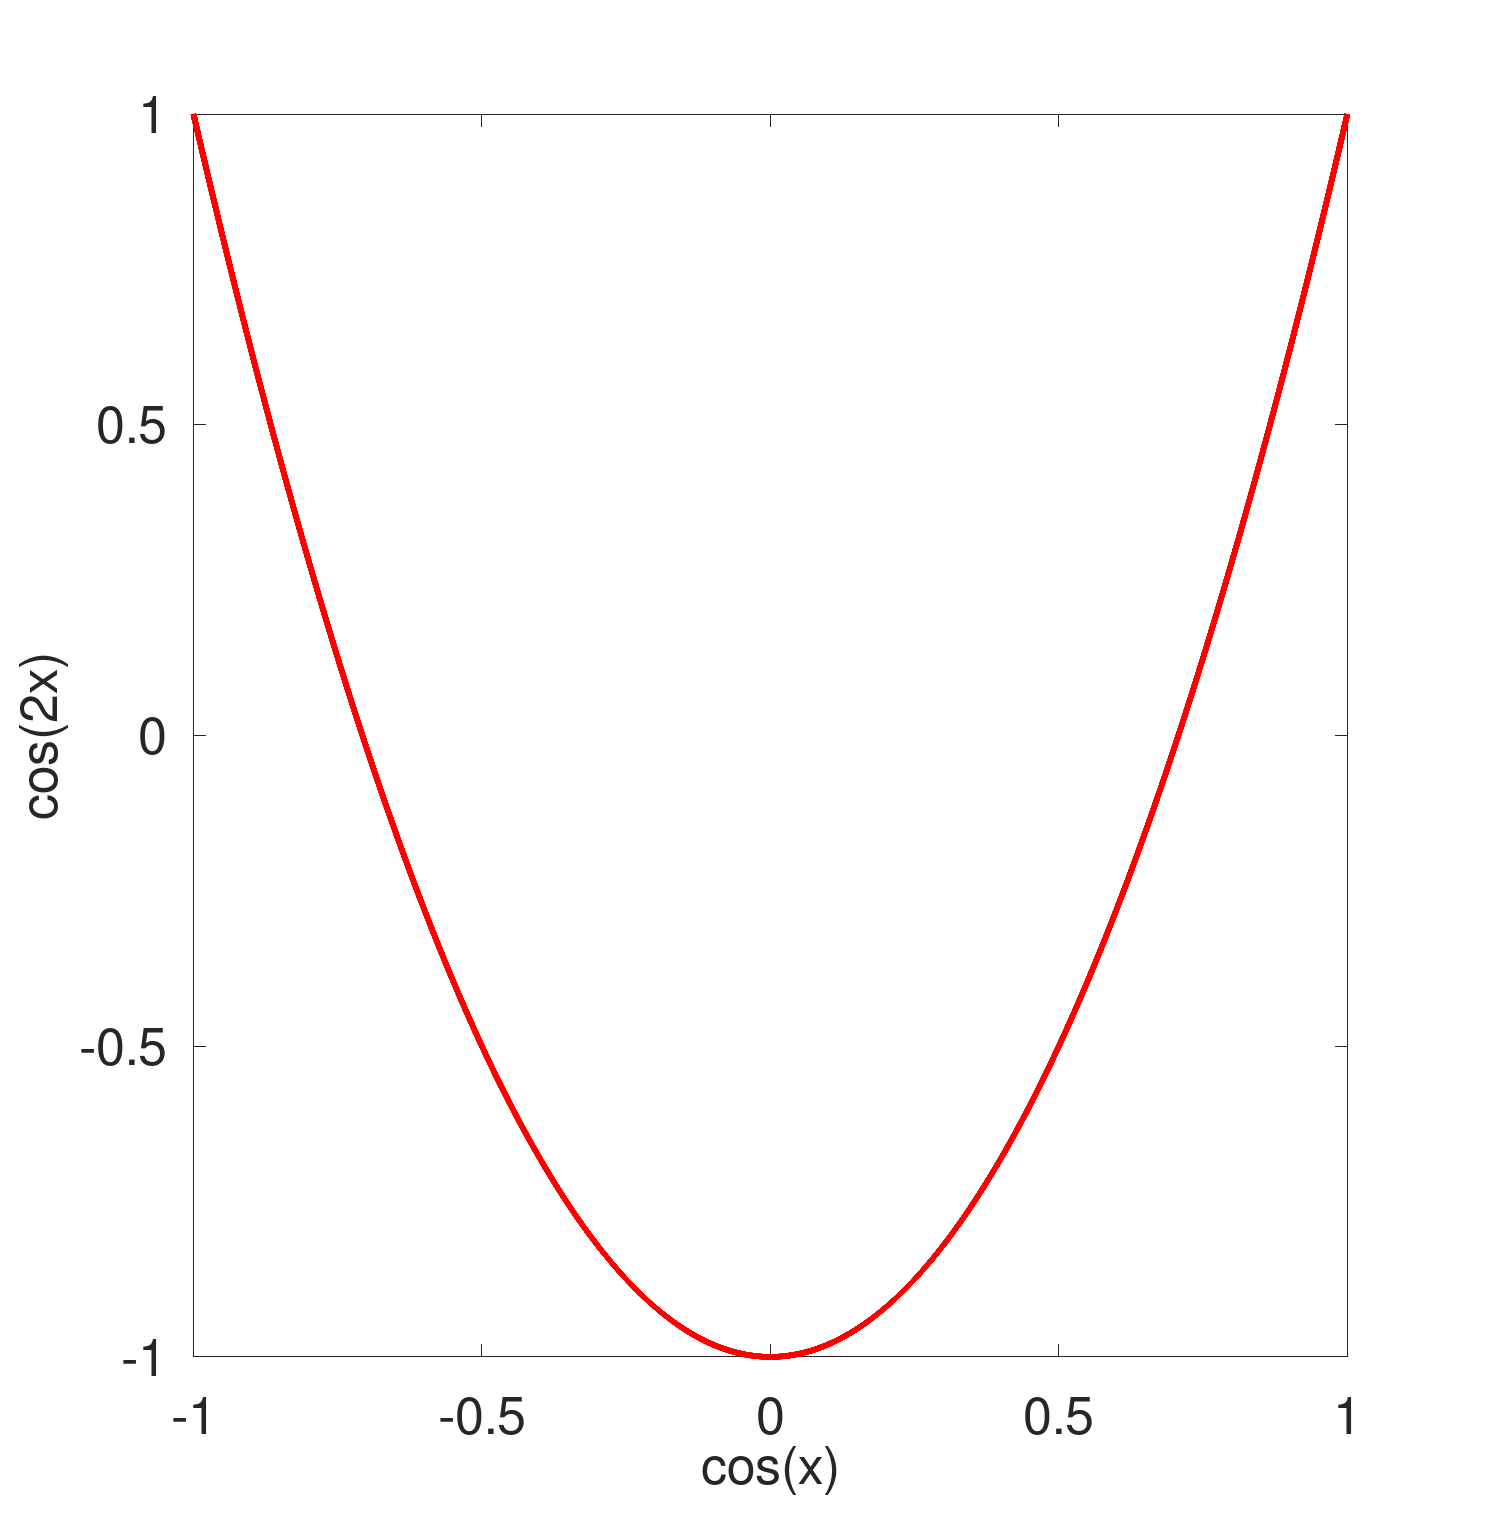
\includegraphics[width=\textwidth]{lissajous4.png}
    \caption{Frequenza 2:1, $\Delta \phi= 0$.}
    \label{fig:third}
\end{subfigure}
\hfill
\begin{subfigure}{0.48\textwidth}
    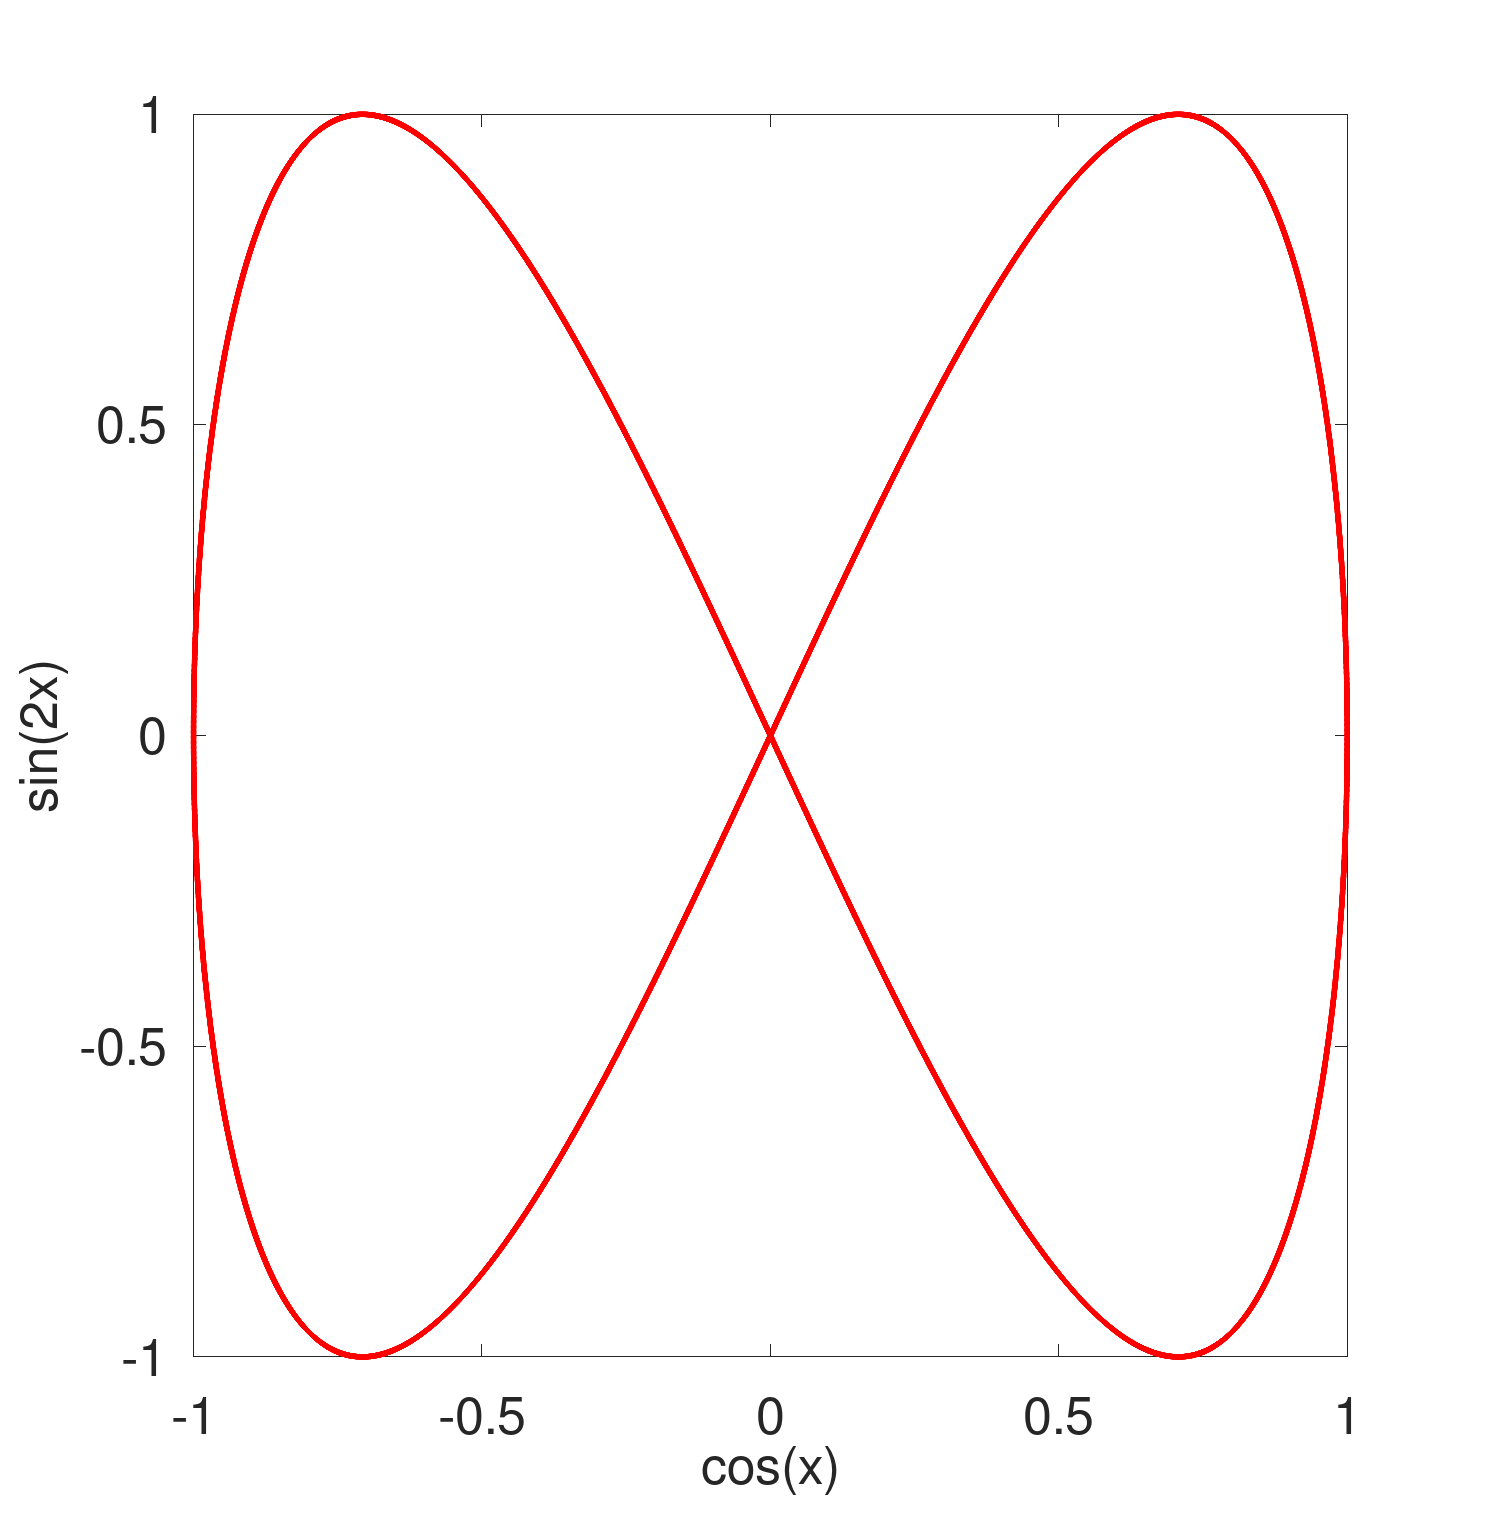
\includegraphics[width=\textwidth]{lissajous3.png}
    \caption{Frequenza 2:1, $\Delta \phi= \frac{\pi}{2}$.}
    \label{fig:first}
\end{subfigure}     
\caption{Figure di Lissajous impiegate.}
\label{fig:lissajous}
\end{figure}
Dal punto di vista della programmazione, l'implementazione di queste figure è estremamente semplice e svolto in pochissime righe come indicato nel listato seguente.
\begin{minted}[frame=lines,framesep=2mm,baselinestretch=1.2,bgcolor=LightGray,fontsize=\footnotesize,linenos]{C}
// Retta
if(joyX > 300 && joyX < 700 && joyY < 300 && switchState == false){
  setX=0.173+0.05*cos(pi*millis()/(vel*2));
  setY=0.133+0.05*cos(pi*millis()/(vel*2));
}

// Cerchio
if(joyX < 300 && joyY < 700 && joyY > 300 && switchState == false){
  setX=0.173+0.05*cos(pi*millis()/(vel*2));
  setY=0.133+0.05*sin(pi*millis()/(vel*2));
}

// Parabola
if(joyX > 300 && joyX < 700 && joyY > 700 && switchState == false){
  setX=0.173+0.05*cos(pi*millis()/(vel*2));
  setY=0.133+0.05*cos(2*pi*millis()/(vel*2));
}

// Infinito
if(joyX > 700 && joyY < 700 && joyY > 300 && switchState == false){
  setX=0.173+0.05*cos(pi*millis()/(vel*2));
  setY=0.133+0.05*sin(2*pi*millis()/(vel*2));
}
\end{minted}
Questa ruotine va a valutare la posizione del joystick tramite le variabili \texttt{joyX}, \texttt{joyY} e il livello di comando tramite la variabile \texttt{switchState}, dove il valore \texttt{false} indica l'analisi di tipo dinamico. Quando una di queste condizioni è verificata, il programma assegna il valore del setpoint con le variabili \texttt{setX}, \texttt{setY} in modo da far muovere la pallina secondo la traiettoria desiderata. La velocità di movimento del setpoint è inversamente proporzionale dalla variabile \texttt{vel}. Si nota come la realizzazione di queste figure è estremamente importante per valutare il comportamento globale del sistema in quanto forniscono tratti curvi e rettilinei, ad alta e bassa velocità.
%La realizzazione del setpoint a movimento circolare è stata precedentemente esposta come esempio nella sezione \ref{sistemidiriferimento} e la sua semplice imlementazione sarà quindi ommessa mentre sarà trattata la realizzazione della funzione $\infty$. É innanzitutto necessario determinare una funzione in coordinate cartesiane che realizzi la figura scelta, analizzando il problema si scopre che la funzione che meglio approssima il simbolo $\infty$ è:
%\begin{equation}\label{infty}
%|y|=|x|\cdot \sqrt{1-|x|}
%\end{equation}
%Notando la presenza dei valori assoluti, per una realizzazione pratica, è necessario scomporre il movimento del setpoint in quattro tratti distinti che assieme realizzano la figura, questo è svolto con il seguente codice:
%Dove la variabile \texttt{draw} viene incrementata a ogni iterazione per determinare la nuova posizione del setpoint che sarà poi assegnata tramite le variabili \texttt{setX} e \texttt{setY}.La funzione $\infty$ in particolare è un ottimo circuito di prova per testare la qualità del controllo in quanto prevede tratti ad alta e bassa velocità in rettilineo e in curva.

\section{Taratura}\label{taratura}
La taratura del controllore PID è un passo critico in quanto determina l'intensità e il tipo di risposta alla posizione della pallina nel piano. Come procedura di taratura si è inizialmente tentato di eseguire manualmente il metodo di Ziegler-Nichols\cite{zieglernichols}\cite{PIDtuningball}, molto comune nei taratori automatici, che però prevede l'impiego di una stima accurata del periodo di oscillazione dell'uscita da stabilizzare. Vista la difficoltà di ricavare questo dato si è quindi preferito procedere ad una taratura euristica andando a valutare individualmente gli effetti delle 3 componenti del PID, questo è svolto incrementando le costanti $K_p$, $K_i$, $K_d$ e valutando l'effetto risultante sul sistema come in tabella \ref{incrementocostanti}.
\begin{table}[h!]
\centering
\resizebox{1\hsize}{!}{$
\begin{tabular}{c|ccccc}
Costante & Stabilità  & Errore a riposo & Velocità risposta & Overshoot  & Tempo stabilizzazione  \\ 
\hline
$K_p$ & Diminuisce & Diminuisce      & Aumenta           & Aumenta    & Non influisce          \\
$K_i$ & Diminuisce & Elimina         & Aumenta           & Aumenta    & Aumenta                \\
$K_d$ & Aumenta    & Non influisce   & Diminuisce        & Diminuisce & Diminuisce            
\end{tabular}$}
\caption{Effetto dell'incremento delle costanti del controllore PID sui parametri di riferimento del sistema.}\label{incrementocostanti}
\end{table}
Si è quindi deciso di procedere nel seguente modo:
\begin{enumerate}
\item La prima componente valutata è stata quella del controllore proporzionale, mantenendo le altre due a $0$, $[K_p,0,0]$, che è stata aumentata fino a garantire una buona escursione al piano in modo da permettere alla palla di raggiungere ogni coordinata.
\item La componente tarata successivamente in modo indipendente, $[0,0,K_d]$, è stata la derivata, anche vista la forte necessità di stabilizzazione, il cui parametro è stato incrementato fino a rendere la posizione della pallina stabile in ogni punto del piano, senza eccedere per evitate un comportamento "nervoso".
\item Infine è stata regolato il comportamento integrale mantenendo costante il proporzionale e al derivativo, $[\overline{K}_p ,K_i, \overline{K}_d]$, che è stato aumentato fino ad annullare l'errore a riposo, permettendo alla pallina di muoversi lentamente fino a raggiungere il setpoint.
\end{enumerate}
Una analisi di fondamentale importanza per valutare questi parametri è stata la risposta allo scalino, ovvero un cambio repentino di setpoint da un valore costante a un altro, che permette di analizzare tutte le componenti della risposta. La combinazione dei tre effetti dà come risultato la risposta allo scalino presente in figura \ref{fig:step}.
\begin{figure}[h!]
\centering

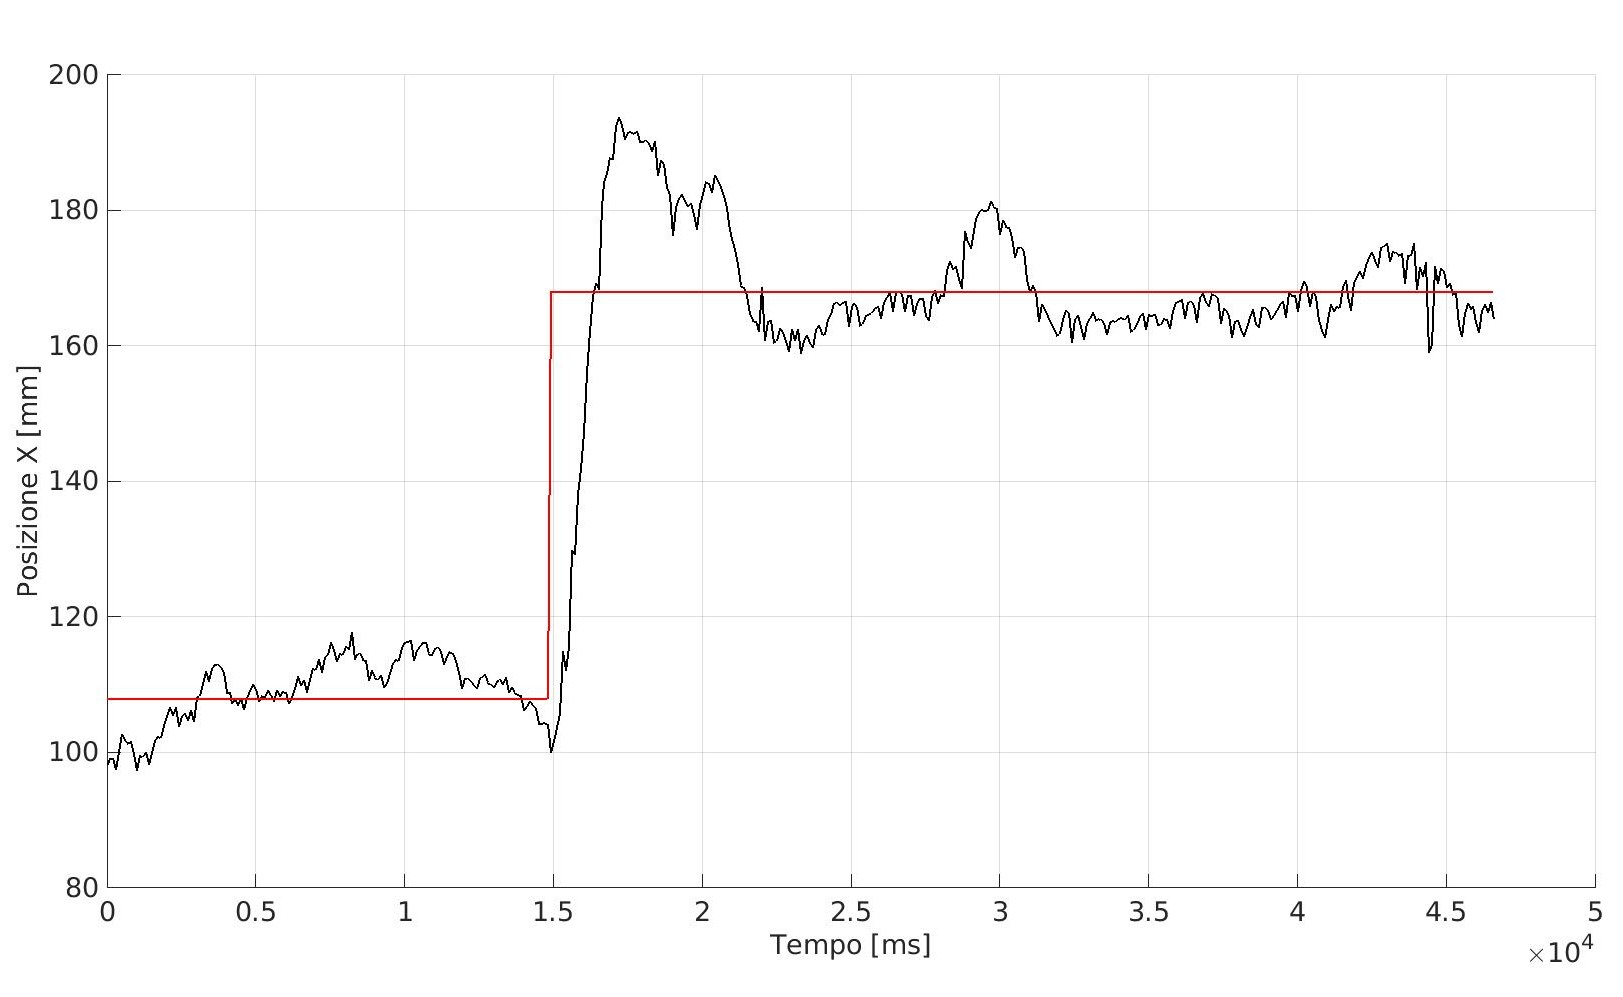
\includegraphics[width=\textwidth]{step2.jpg}

\caption{Risposta allo scalino del sistema lungo l'asse $x$.} \label{fig:step}
\end{figure}
Come si può notare la risposta del sistema è veloce, senza un eccessivo overshoot e un discreto assestamento del valore sul setpoint, in particolare, in condizioni statiche il sistema è in grado di mantenere la pallina perfettamente centrata sul valore desiderato entro un margine di errore di soli $10mm$.
\chapter{Risultati}\label{risultati}
Vista la complessità del progetto e la diversità dei parametri valutativi i risultati saranno espressi separatamente per la piattaforma di Stewart e per il piano stabilizzato rispettivamente nelle sezioni \ref{resultstewart} e \ref{resultpiano}.
\section{Piattaforma di Stewart}\label{resultstewart}
Il controllo della piattaforma di Stewart può essere valutato in base alle capacità di movimento permesse dai sei gradi di libertà. I test eseguiti per valutare queste capacità sono stati:
\begin{itemize}
\item L'assegnazione di funzioni sinusoidali ai valori di $x,y,z$ in modo da valutare sia l'escursione verticale, sia la capacità di movimento orizzontale.
\item L'assegnazione di angoli compresi tra i $\pm 5^\circ$ alle componenti di rollio e beccheggio per testare il range di inclinazione del piano, importantissimo nella successiva fase di controllo della palla.
\item L'assegnazione di una escursione di $\pm 15^\circ$ all'imbardata per verificarne il corretto funzionamento.
\end{itemize}
Tutti questi test hanno avuto successo e la piattaforma ha dimostrato un'ottima fluidità nei movimenti, è stato quindi possibile procedere all'implementazione del piano resistivo.
\section{Piano stabilizzato}\label{resultpiano}
Nella sezione \ref{taratura} è stata esposta la procedura seguita per tarare il sistema e la conseguente risposta al gradino. Questo già di per sé costituisce un ottimo risultato e una dimostrazione delle capacità di controllo ma sono necessari ulteriori test per valutarne a pieno le capacità. Nella sezione \ref{assegnazionecomandi} sono state indicate le procedure per far seguire al setpoint le curve delle figure di Lissajous, queste sono certamente più interessanti e permettono di valutare la precisione del sistema con una velocità di movimento fissata del setpoint. Per valutare questo aspetto è stato scritto un semplice script \texttt{MATLAB} che legge la posizione della palla da un file CSV prodotto da Arduino e la riporta in un grafico a dispersione $(x,y)$ su cui viene poi sovrapposto il tracciato esatto compiuto dal setpoint. I risultati del tracking delle varie curve sono riportati nelle figure \ref{fig:c1}, \ref{fig:r1}, \ref{fig:u1} e \ref{fig:i1} dove sono mostati sovrapposti i tracciati di diversi periodi del moto per valutarne la consistenza. Si nota immediatamente che i tracciati non seguono perfettamente la curva descritta dal setpoint ma sembrano deviare su una traiettoria diversa, questo è dovuto a due fattori principali: 
\begin{itemize}
\item Per eseguire l'analisi dinamica si sacrificano alcuni parametri importanti nell'analisi statica, come le componenti integrale e derivativa del controllore PID per permettere una maggiore fluidità di movimento a scapito della precisione del tracking.
\item La fondamentale asimmetria della risposta dei servomotori nell'eseguire le operazioni di rollio e beccheggio a causa della disposizione esagonale degli attuatori che provoca una diversa risposta in frequenza lungo gli assi $x$ e $y$.
\end{itemize}
La presenza dell'asimmetria nella risposta in frequenza si può facilmente notare analizzando le figure di Lissojous, in particolare valutando la figura \ref{fig:r1}, dove l'interpolazione dei punti tracciati dalla palla suggerisce uno sfasamento nella risposta di circa $10^\circ$, questo può quindi essere compensato per avere delle figure corrette.
Nella figura \ref{fig:phasecorr} sono mostrati i tracciati ottenuti sfasando di $10^\circ$ la componente verticale rispetto alla orizzontale, dove si nota un particolare miglioramento nella realizzazione delle figure della parabola e dell'infinito, che risultano essere più consistenti con il tracciato previsto.
Analizzando i tracciati, si può notare una dispersione sulle ripetizioni, comunque limitata ad un margine di $2cm$, nonostante questo la figura si mantiene e non si verificano perdite di controllo. Si può inoltre notare come la velocità della pallina sia direttamente collegata all'overshoot del setpoint, questo è chiaramente visibile in figura \ref{fig:ic1}, dove l'intersezione è percorsa in modo molto consistente mentre agli estremi, dove la velocità è maggiore, si ha un incremento nel distacco. Lo stesso può essere visto in figura \ref{fig:rc1}, dove la pallina compie un overshoot prima di arrestarsi e cambiare direzione. %Un altro fattore da valutare è l'asimmetria di alcune figure come la \ref{fig:u1} e al \ref{fig:i1} dove il lato destro e sinistro sono diversi nonostante il setpoint sia perfettamente simmetrico. Questi fattori sono dovuti principalmente alla natura stessa dell'analisi dinamica, in quanto i fattori derivativo e integrale devono essere ridotti in modo sostanziale per avere un movimento fluido, a scapito appunto dell'overshoot e della compensazione dell'angolo di inclinazione a riposo.
%Si nota in particolare come per eseguire queste figure dinamicamente sia necessario modificare sostanzialmente i parametri del PID, riducendo i parametri derivativo e integrativo per avere una maggiore fluidità e velocità di movimento a scapito della precisione.
\begin{figure}[h!]
\centering
\begin{subfigure}{0.49\textwidth}
    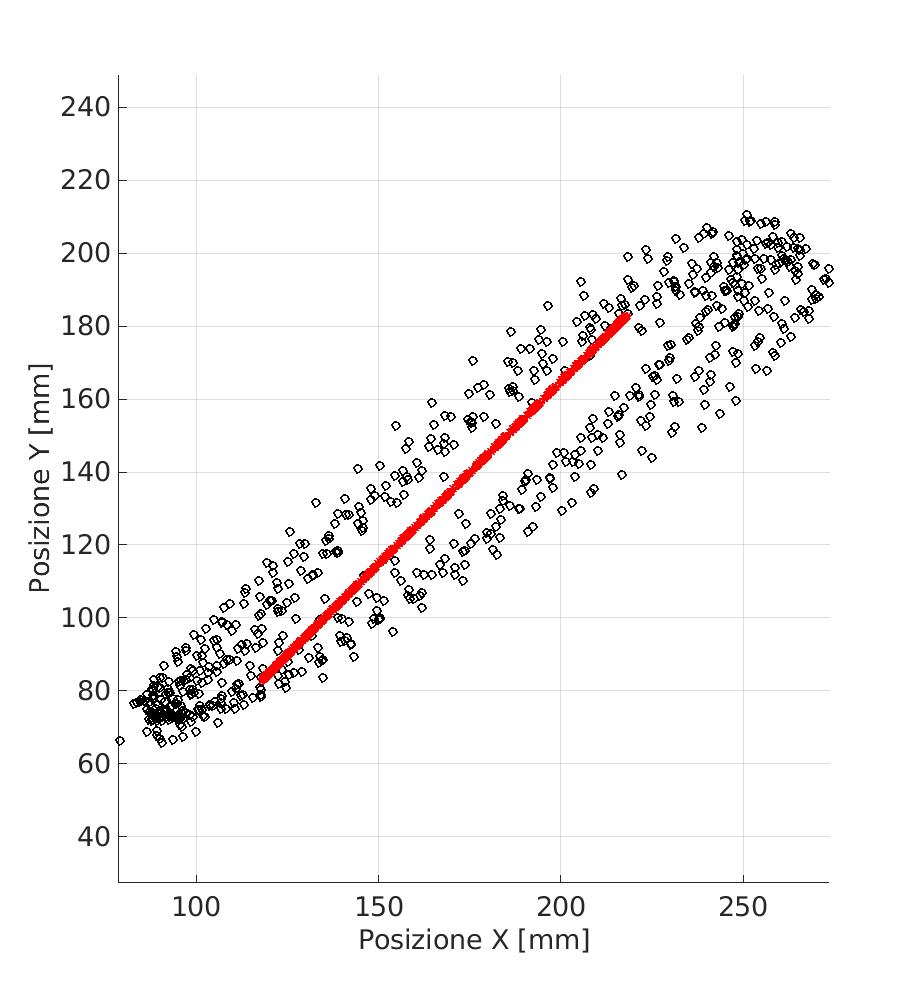
\includegraphics[width=\textwidth]{rn.jpg}
    \caption{Frequenza 1:1, $\Delta \phi= 0$.}
    \label{fig:r1}
    \vspace*{10mm}
\end{subfigure}
\hfill
\begin{subfigure}{0.49\textwidth}
    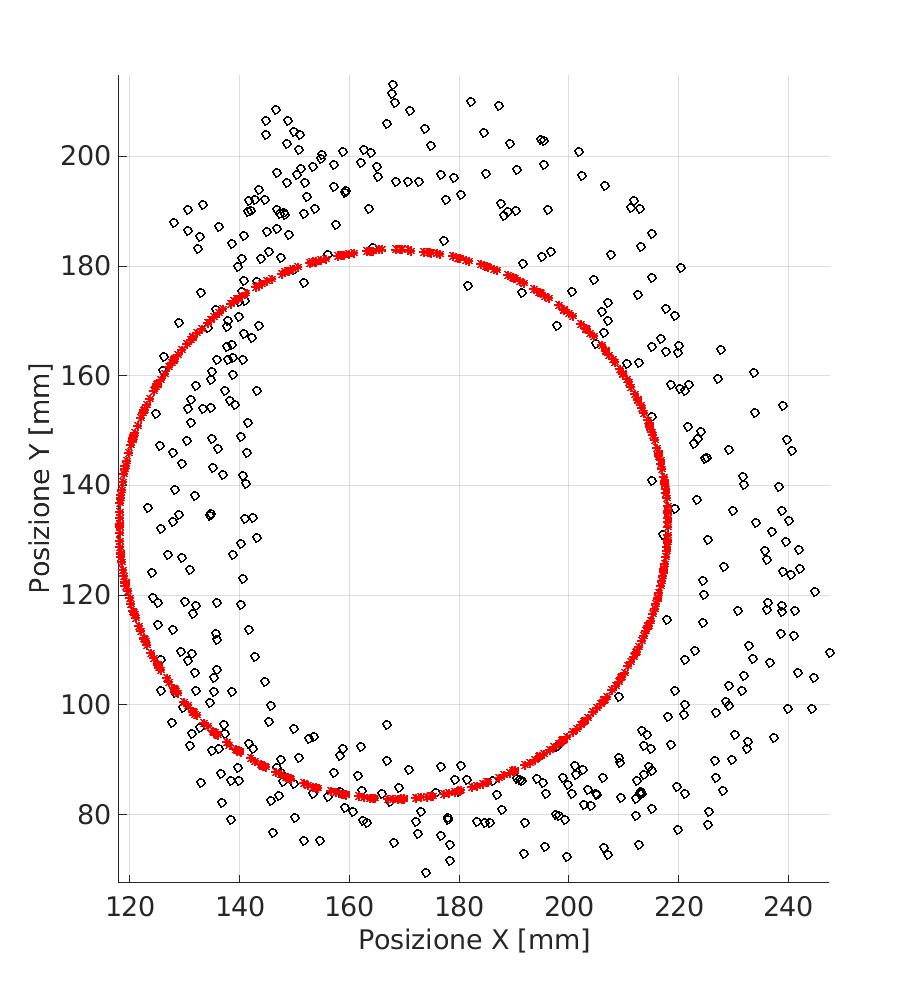
\includegraphics[width=\textwidth]{cn.jpg}
    \caption{Frequenza 1:1, $\Delta \phi= \frac{\pi}{2}$.}
    \label{fig:c1}
    \vspace*{10mm}
\end{subfigure}
\hfill
\begin{subfigure}{0.49\textwidth}
    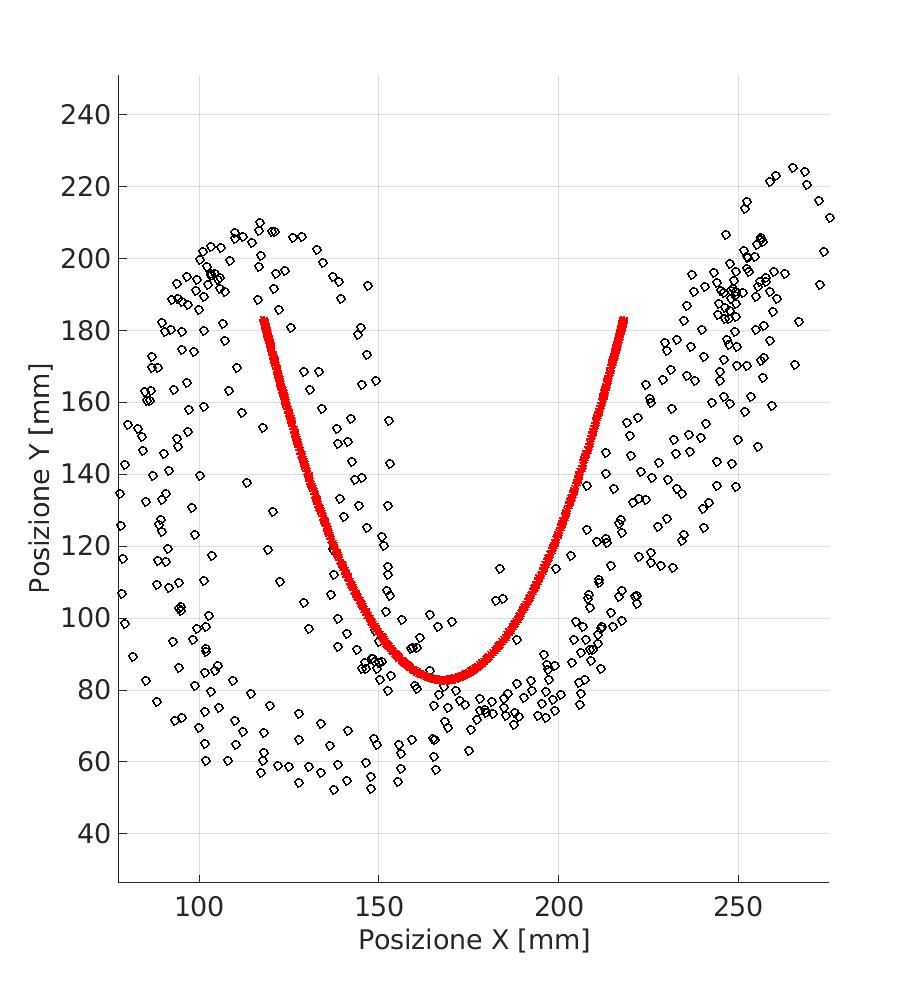
\includegraphics[width=\textwidth]{un.jpg}
    \caption{Frequenza 2:1, $\Delta \phi= 0$.}
    \label{fig:u1}
\end{subfigure}
\hfill
\begin{subfigure}{0.49\textwidth}
    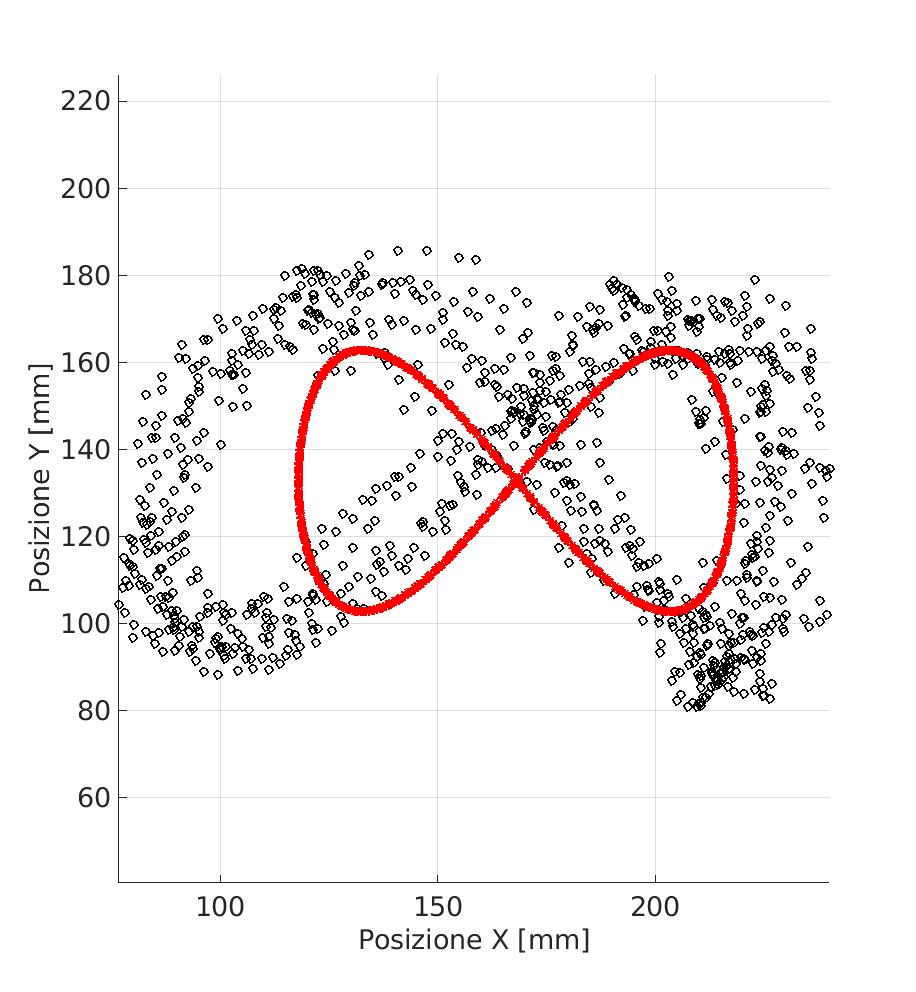
\includegraphics[width=\textwidth]{in.jpg}
    \caption{Frequenza 2:1, $\Delta \phi= \frac{\pi}{2}$.}
    \label{fig:i1}
\end{subfigure}     
\vspace*{10mm}
\caption{Tracciati registrati senza compensare la fase.}
\label{fig:lissajous2}
\end{figure}
\newpage
\begin{figure}[h!]
\centering
\begin{subfigure}{0.49\textwidth}
    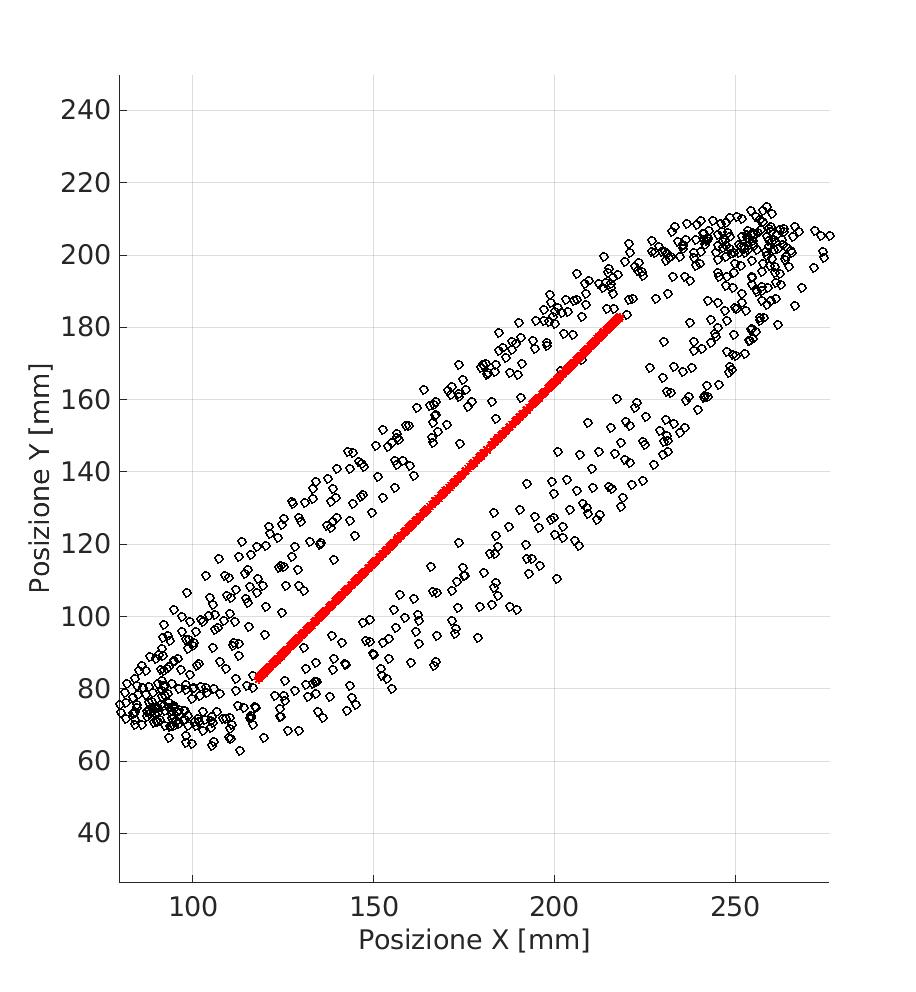
\includegraphics[width=\textwidth]{rc.jpg}
    \caption{Frequenza 1:1, $\Delta \phi= 0$.}
    \label{fig:rc1}
    \vspace*{10mm}
\end{subfigure}
\hfill
\begin{subfigure}{0.49\textwidth}
    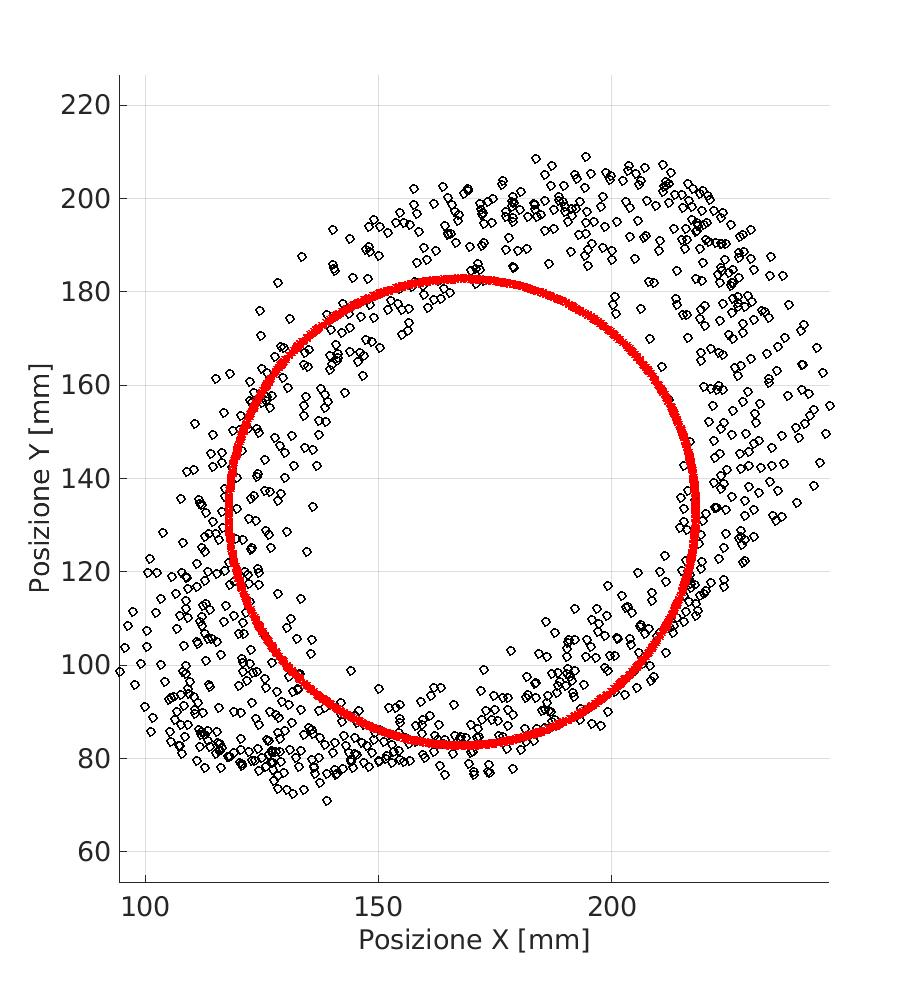
\includegraphics[width=\textwidth]{cc.jpg}
    \caption{Frequenza 1:1, $\Delta \phi= \frac{\pi}{2}$.}
    \label{fig:cc1}
    \vspace*{10mm}
\end{subfigure}
\hfill
\begin{subfigure}{0.49\textwidth}
    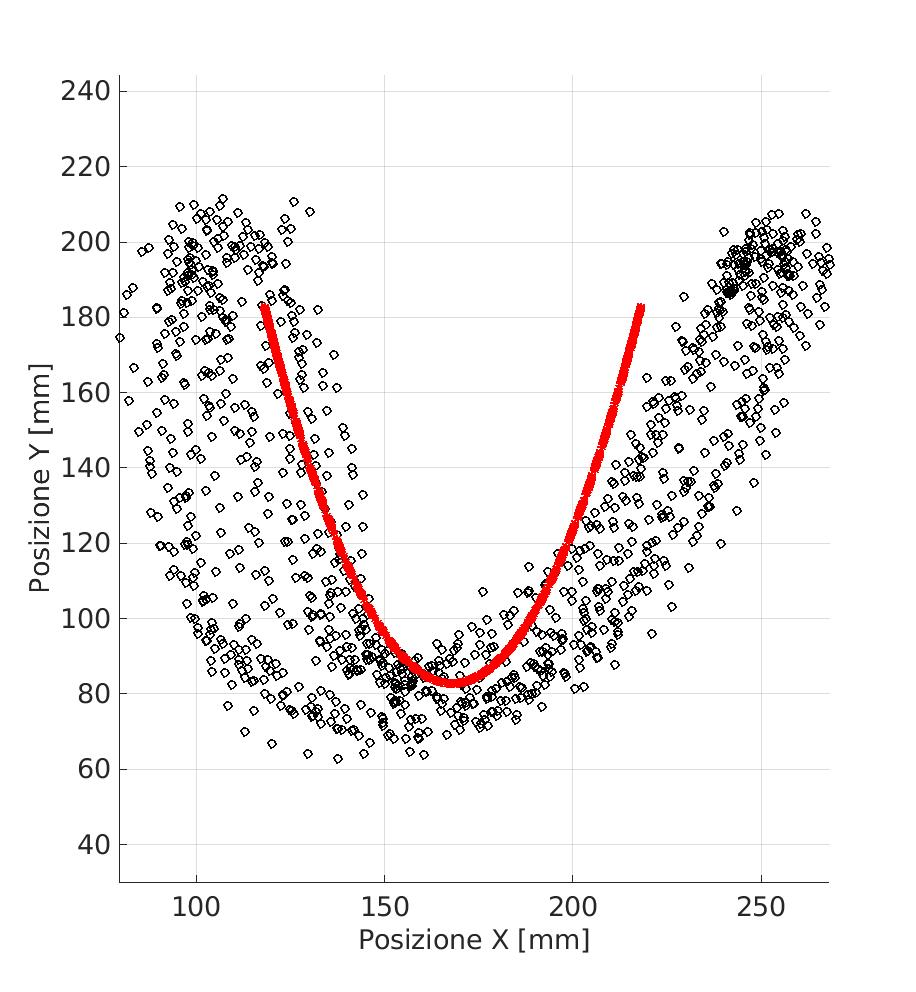
\includegraphics[width=\textwidth]{uc.jpg}
    \caption{Frequenza 2:1, $\Delta \phi= 0$.}
    \label{fig:uc1}
\end{subfigure}
\hfill
\begin{subfigure}{0.49\textwidth}
    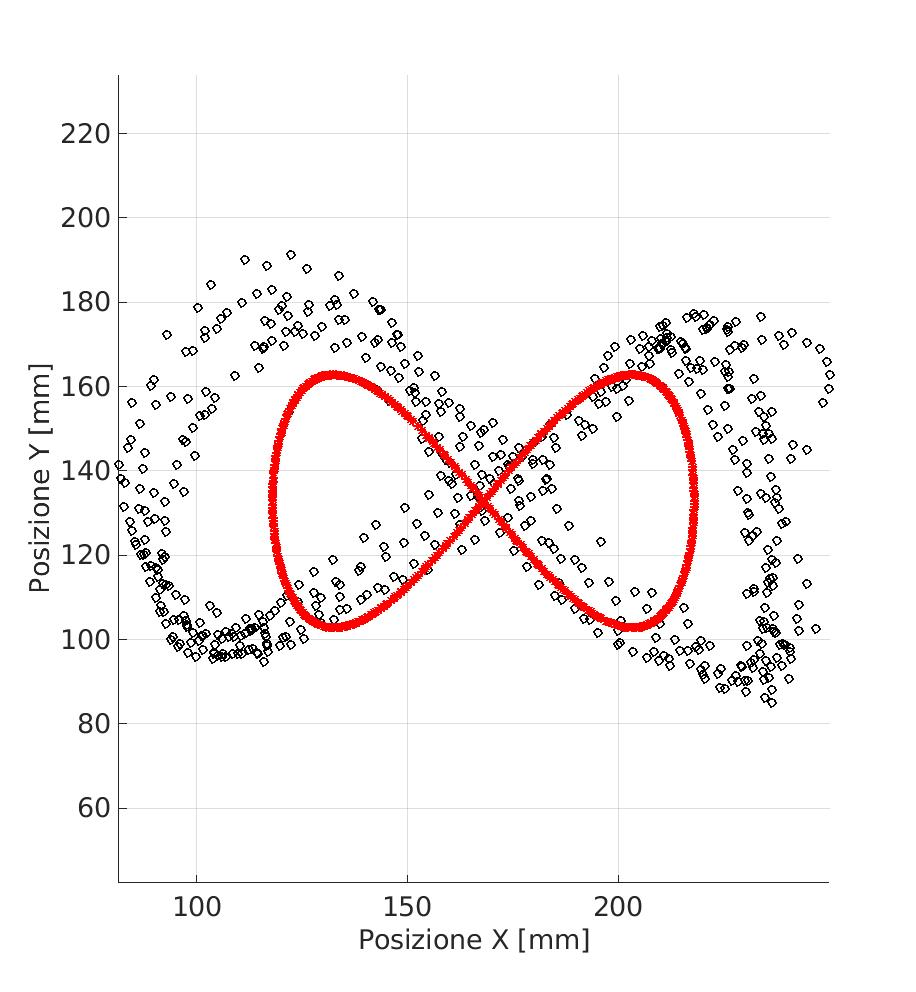
\includegraphics[width=\textwidth]{ic.jpg}
    \caption{Frequenza 2:1, $\Delta \phi= \frac{\pi}{2}$.}
    \label{fig:ic1}
\end{subfigure}     
\vspace*{10mm}
\caption{Tracciati registrati compensando la fase.}
\end{figure}
\label{fig:phasecorr}


\chapter{Conclusioni}
L'obiettivo prefissato era di realizzare una piattaforma di Gough-Stewart con attuatori rotativi ed un relativo sistema di controllo in grado di stabilizzare una pallina sul piano e valutarne il comportamento dinamico. %Questo obbiettivo è stato raggiunto, come provato nelle sezioni \ref{resultstewart} e \ref{resultpiano}, che dimostrano le ottime capacità di controllo e ripetibilità, ottenute nei vari casi di studio. 

Il raggiungimento di questo risultato si è ottenuto gradualmente, studiando, analizzando e testando ogni aspetto del progetto; partendo dai singoli componenti elettronici e arrivando infine ad un risultato concreto.
La prima fase è stata attuata studiando le tecnologie impiegate, i loro vantaggi, svantaggi e la loro compatibilità, che ha portato alla realizzazione di un opportuno chip di controllo per il pilotaggio del piano resistivo. Successivamente si è proceduto allo studio della piattaforma di Gough-Stewart, analizzandola dal punto di vista matematico, costruendo un modello che ne permettesse una rappresentazione opportuna e un idoneo algoritmo che ne risolvesse il problema cinematico inverso. Una volta conclusa questa fase di studio preliminare si è potuto procedere all'assemblaggio della piattaforma e all'implementazione degli algoritmi in linguaggio \texttt{C} che ha da subito riportato ottimi risultati, come indicato nella sezione \ref{resultstewart}. Basandosi su questo risultato è stato possibile procedere al montaggio del piano resistivo alla piattaforma, tramite agganci opportunamente realizzati. Per risolvere il problema di stabilizzazione è stato necessario un attento studio del modello del piano e del controllore PID, valutando opportune modifiche per ottenere un controllo ottimale.  Il passo successivo è stata la programmazione della logica di controllo, il filtraggio dei dati in ingresso dal digitalizzatore resistivo e un algoritmo di assegnazione del setpoint che permettesse di valutare le prestazioni del sistema. Si è dato poi seguito ad una opportuna operazione di taratura euristica del controllore, tramite la valutazione della risposta allo scalino, presente in figura \ref{fig:step}. Unendo tutti questi aspetti progettuali si è giunti allo studio dell'analisi dinamica, esposto in dettaglio nella sezione \ref{resultpiano}, dove si è notato e corretto uno sfasamento della risposta in frequenza lungo gli assi. 

Gli obiettivi posti sono quindi stati rispettati e il sistema ha dimostrato ottime capacità di controllo e ripetibilità nei vari casi di studio. 

Ulteriori miglioramenti delle prestazioni del sistema si potrebbero ottenere impiegando tecnologie più sofisticate e controllori più avanzati.
In particolare, l'impiego di un piano capacitivo al posto del resistivo offrirebbe degli indubbi vantaggi, passando da un'attuazione di tipo meccanico ad una elettromagnetica, la quale avrebbe un impatto drastico sui disturbi e sulla precisione di rilevazione della posizione. Questo inoltre non andrebbe ad alterare in alcun modo la traiettoria della pallina, in quanto presenterebbe una superficie totalmente liscia, a differenza del piano resistivo che è caratterizzato alcune irregolarità a causa dei separatori tra i due strati conduttivi. A livello di controllo si nota come sia preferibile impiegare tecniche fuzzy\cite{tecnichecontrollo} che permettono di avere risposte più rapide e un minore overshoot rispetto a un controllore PID tradizionale.


%Miglioramenti possono essere apportati per incrementare le prestazioni del sistema, questi riguradano principalmente l'hardware ed in particolare il piano resistivo. Tramite l'impiego di un digitalizzatore capacitivo sarebbe possibile passare da un'attuazione meccanica ad una elettromagnetica, rimuovendo le irregolarità nel piano dovute ai separatori, le quali sono correlate ai disturbi nel segnale relativo alla posizione (figura \ref{fig:filtraggioposizione}), permettendo una migliore precisione e stabilità. 



%AGGIUNGERE BIBLIOGRAFIA
%\bibliographystyle{alpha}
%\bibliography{references} % see references.bib for bibliography management
\newpage
\addcontentsline{toc}{section}{\refname}
%\nocite{*}
\printbibliography
\end{document}


